\documentclass[pdftex,10pt,b5paper,twoside]{book}
\usepackage{geometry} 	% Better geometry
\geometry{b5paper}
\usepackage[norsk]{babel} %gir oss norske oversettelser
\addto\captionsnorsk{%
  \renewcommand\appendixname{Vedlegg}
  \renewcommand\appendixpagename{Vedlegg}
  \renewcommand\appendixtocname{Vedlegg}
}

\addto\extrasnorsk{%
  \def\chapterautorefname{Kapittel}%
}



\usepackage{pdfpages} % slik at pdf filer kan legges til i rapporten

\usepackage[utf8]{inputenc}
\usepackage{todonotes} %gjør det mulig å legge til todo-notater
\usepackage[pdftex]{hyperref} %gjør det mulig å skrive nettadresser
\newcommand\fnurl[2]{%
  \href{#2}{#1}\footnote{\url{#2}}%
} %nettadresser i fotnoter
\usepackage{graphicx} %gir støtte for bilder
\usepackage[font={small,it}]{caption} %gjør bildeteksten annerledes enn annen tekst (mindre og i kursiv)
\usepackage{mdwlist} %gjør det mulig å suspende og resume enumerate lister

\usepackage[toc,page]{appendix} %for å lage vedlegg

\usepackage{tabularx}
\usepackage{booktabs}%for å få finere tabeller

{\renewcommand{\arraystretch}{1.5}
\usepackage{framed} % lage boxer

%\usepackage[hang]{subfigure} % gjør det mulig å ha to bilder i en figur
\usepackage{subcaption}
\usepackage[acronym, toc]{glossaries}
\makeglossaries
\usepackage{longtable} %gjør det mulig å ha tabeller som går over flere sider
\usepackage{multirow} %gjør det mulig med multirows

\usepackage{parskip} %gir avsnitt med mellomrom mellom linjene istedenfor sånne teite innrykk
\usepackage{microtype} %gjør at linjeskift skjer på bedre steder
\usepackage{float}
\usepackage[T1]{fontenc}

\usepackage[babel=true]{csquotes}

\usepackage[
    backend=biber
     ,style=authoryear    % Alphabeticalsch
     %,style=numeric-comp  % numerical-compressed
     ,sorting=none        % no sorting
     ,sortcites=true      % some other example options ...
     ,block=none
     ,indexing=false
     ,citereset=none
     ,isbn=true
     ,url=true
     ,doi=true            % prints doi
     ,natbib=true         % if you need natbib functions
]{biblatex}
\bibliography{mylib}

\usepackage{setspace} %for p kunen øke linjeavstanden
\onehalfspacing %øker linjeavstanden


\newcommand{\thesisAuthor}{Anette Ellingsberg, Dagrun Haugland og Hanne Kottum}
\newcommand{\thesisTitle}{Visualisering av personlig legemiddelinformasjon}
\newcommand{\thesisType}{MASTEROPPGAVE}
\newcommand{\thesisDate}{Vår 2015}
\newcommand{\thesisRQ}{\begin{quote} Kan en visuell fremstilling av personlig legemiddelinformasjon gi pasienter raskere svar på spørsmål, og mer korrekt kunnskap, om interaksjoner og bivirkninger knyttet til egne legemidler, enn tekst i pakningsvedlegg?\end{quote}}
% PDF info
\hypersetup{pdfauthor={\thesisAuthor}}
\hypersetup{pdftitle={\thesisTitle}}
\hypersetup{pdfsubject={\thesisType}}

\raggedbottom
\begin{document}

%Title page (This is generate automatically from the commands above)
\thispagestyle{empty}


\Huge{\textbf \thesisTitle}\\[1pc]
\Large{En eksperimentell sammenligning av prototypesystem og pakningsvedlegg}\\[1pc]

\begin{center}

\Large{\thesisAuthor}\\[1pc]
\Large{\thesisDate}\\[4pc]

\thesisType\\ [2pc]
Institutt for datateknikk og informasjonsvitenskap\\
Norges teknisk-naturvitenskapelige universitet \\ [2pc]

\includegraphics[width=3cm]{fig/logo_ntnu_u-slagord.png} \\[3pc]
\end{center}


\vfill


\small{Veileder: Øystein Nytrø \\
Biveiledere: Rune Sæter, Jens Lien, Janne Sund \& Marley Kristin Singarajah}

 % Forside


\thispagestyle{empty}

\cleardoublepage


%% PART 1 -- ting som kommer før innholdsfortegnelse
\pagenumbering{gobble}
\chapter*{Sammendrag}
\addcontentsline{toc}{chapter}{Sammendrag}
\pagenumbering{roman} 				
\setcounter{page}{1}

Bruk av legemidler er et viktig tiltak i helsevesenet, men er ofte lite koordinert og ikke underlagt samlet kontroll. Denne mangelen på koordinering kan føre til at pasienters legemiddelbehandling ikke blir så god som den kunne vært. At pasienten selv har oversikt over egen legemiddelsituasjon, og tilgang til informasjon om denne, kan gi bedre forutsetninger for å påse at legemiddelbehandlingen blir optimal. Pasienter har tilgang til flere legemiddelinformasjonskilder, men disse er ikke personlig tilpasset og bruker ofte språk som krever forståelse av medisinske ord og uttrykk. 

Det overordnede målet med masteroppgaven var å gjøre personlig legemiddelinformasjon lettere tilgjengelig for pasienter enn i dag. Følgende forskningsspørsmål ble besvart: 
\thesisRQ

Det ble utviklet en prototype av et interaktivt system, med en visuell fremstilling av personlig legemiddelinformasjon. Formålet med prototypen var å bruke den i et eksperiment for å besvare forskningsspørsmålet. Eksperimentet sammenlignet  prototypen med pakningsvedlegg for å undersøke om bruk av prototypen gjorde pasienter i stand til å finne informasjon raskere, besvare spørsmål riktigere og oppnå større læringsutbytte enn ved bruk av pakningsvedlegg. 

Konklusjonen av eksperimentet var at prototypen gir raskere svar på spørsmål, og mer korrekt kunnskap, om bivirkninger og interaksjoner, enn tekst fra pakningsvedlegg.
\chapter*{Abstract}
\addcontentsline{toc}{chapter}{Abstract}

The use of drugs is an important measure in the public health service, but it is often poorly coordinated and rarely placed under assembled control. The lack of coordination may result in patient drug treatments that are less than optimal for some patients. Patients with an overview of their own drug use, and access to this information on a daily basis, can achieve better premises for obtaining an optimal drug treatment. Today patients have access to multiple drug information sources, but these are not personalized and often use a language that require an understanding of medical terms.      

The overall objective of this thesis was to make personal drug information easier accessible for patient than it is today. This thesis aims to answer the following research question:
\begin{quote} Can visual representation of personal drug information provide patients with answers to questions faster, and provide them with more correct knowledge, about drug-drug interactions and side effects, than text from patient information leaflets?\end{quote}

A prototype of an interactive system containing a visual representation of personal drug information was developed. The prototype was used in an experiment with the purpose of answering the research question. The experiment compared the prototype to patient information leaflets. It exanimated if patient were able to find information faster, answer questions more correctly and obtain a higher learning outcome with the use of the prototype, then with the use of patient information leaflets.

The experiment concluded that the prototype provides patients with answers to questions faster, and provide them with more correct knowledge, about drug-drug interactions and side effects, than text from patient information leaflets.


\chapter*{Forord}
\addcontentsline{toc}{chapter}{Forord}

Denne masteroppgaven ble utført ved NTNU, Institutt for datateknikk og informasjonsvitenskap, i perioden januar til juni, 2015. 
Masteroppgaven er i sin helhet et felles arbeid utført av Anette Ellingsberg, Dagrun Haugland og Hanne Kottum. 

Vi vil gjerne takke Øystein Nytrø for kyndig veiledning, råd og diskusjoner underveis. Vi vil også takke Rune Sætre, Jens Lien, Janne Sund og Marley Kristin Singarajah for veiledning og oppfølging. Takk til Cecilie Wold for gode innspill. \\ \mbox{}\\[4pc]

Trondheim, juni 2015\\
Anette Ellingsberg, Dagrun Haugland og Hanne Kottum

\clearpage


%% PART 2 Innholdsfortegnelse
\tableofcontents
\addcontentsline{toc}{chapter}{Innhold}
\clearpage




 %%lager innholdsfortegnelse

%ordliste og forkortelser:
\newglossaryentry{legemiddel}
{
    name=Legemidler,
    description={er, i henhold til legemiddelloven § 2, “(...)stoffer, droger og preparater som er bestemt til eller utgis for å brukes til å forebygge, lege eller lindre sykdom, sykdomssymptomer eller smerter, påvirke fysiologiske funksjoner hos mennesker eller dyr, eller til ved innvortes eller utvortes bruk å påvise sykdom”}
}

\newglossaryentry{symptom}
{
    name=Symptom,
    description={er en “(...)subjektiv opplevelse av at noe er unormalt med en selv” \citep{LeksikonSymptom}. Et symptom kan være et av tegnene på en sykdom. Hodepine er et eksempel på et symptom}
}
\newglossaryentry{tegn}
{
    name=Tegn,
    description={er observerbare eller registrerbare symptomer. Tegn kan være synlige eller kan oppdages ved hjelp av medisinske tester. Høyt blodtrykk er et eksempel på et tegn}
}
\newglossaryentry{indikasjon}
{
    name=Indikasjon,
    description={er årsaken til å ta et legemiddel. Et legemiddel kan ha flere indikasjoner. Diabetes type 2 er et eksempel på en indikasjon for Amaryl}
}
\newglossaryentry{generiske legemidler}
{
    name=Generiske legemidler,
    description={er medisinsk likeverdige legemidler fordi de inneholder samme virkestoff i samme styrke. Legemidlene kan ha forskjellige handelsnavn, hjelpestoffer, farge, form og forpakning}
}
\newglossaryentry{effekt}
{
    name=Effekt,
    description={er virkningen et legemiddel har på pasienten som tar legemiddelet}
}
\newglossaryentry{bivirkning}
{
    name=Bivirkning,
    description={er en ikke-tilsiktede effekt et legemiddel kan ha}
}
\newglossaryentry{interaksjon}
{
    name=Interaksjon,
    description={er at legemidler, legemidler og helsekostprodukter, legemidler og mat, eller legemidler og drikke, påvirker hverandre}
}
\newglossaryentry{atc-def}
{
    name=Anatomical Therapeutic Chemical,
    description={er en klassifisering av legemidler ut i fra hvilket organ de virker på, og ut i fra legemidlets kjemiske, farmakologiske og terapeutiske karakteristikk}
}
\newglossaryentry{ICD-def}
{
    name=ICD,
    description={er koder for klassifisering av sykdommer og beslektede helseproblemer}
}
\newglossaryentry{mengde}
{
    name=Mengde,
    description={er antall enheter per inntak av et legemiddel}
}
\newglossaryentry{Styrke}
{
    name=Styrke,
    description={av et legemiddel er innholdet av virkestoff per enhet}
}
\newglossaryentry{Dose}
{
    name=Dose,
    description={er det totale innholdet av virkestoff per inntak av et legemiddel. \(Dose = mengde \times styrke\). En pasient som tar 2 tabletter(mengde) av et legemiddel med styrke på 50 mg tar en dose på 100 mg} 
}
\newglossaryentry{diagnose}
{
    name=Diagnose,
    description={er en sykdoms art og navn. Diagnose stilles på grunnlag av opplysninger om pasienten og av de funn gjort ved en kliniske undersøkelse} 
}
\newglossaryentry{legemiddelgjennomgang}
{
    name=Legemiddelgjennomgang,
    description={er en “strukturert/systematisk evaluering av den enkelte pasientens legemiddelregime i den hensikt å optimalisere effekten av legemidlene og redusere risiko ved legemiddelbruk” \citep{legemiddelgjennomgang}} 
}
\newglossaryentry{elektronisk pasientjournal}
{
    name=Elektronisk pasientjournal,
    description={er et datasystem som inneholder alle opplysninger tilgjengelig i en pasientjournal. En elektronisk pasientjournal inneholder helseopplysninger, prøvesvar, spesialundersøkelser, arbeidsdokumenter og øvrige dokumenter knyttet til pasienten. Elektroniske pasientjournaler kan også inneholde informasjon fylt inn av pasienten selv} 
}
\newglossaryentry{elektronisk resept (e-resept)}
{
    name=Elektronisk resept (e-resept),
    description={er en resept som ikke skrives ut på papir, men som en fysisk eller juridisk person med rett til å rekvirere legemidler sender elektronisk til en sentral reseptdatabase} 
}
\newglossaryentry{etterlevelse}
{
    name=Etterlevelse,
    description={er et begrep som brukes for å beskrive hvorvidt legemidler tas som foreskrevet eller ikke } 
}
\newglossaryentry{fastlege}
{
    name=Fastlege,
    description={er en allmennpraktiserende lege med formell avtale med kommunen om et varig forhold mellom legen og pasientene. Fast legen skal tilby alle pasientene på sin liste alle typer “allmennlegeoppgaver”}
}
\newglossaryentry{helseopplysninger}
{
    name=Helseopplysninger,
    description={er “... taushetsbelagte opplysninger i henhold til helsepersonelloven § 21 og andre opplysninger og vurderinger om helseforhold eller av betydning for helseforhold, som kan knyttes til en enkeltperson”}
}
\newglossaryentry{ordinering}
{
    name=Ordinering,
    description={er at legen bestemmer bruk av legemiddel og dosering, og journalfører dette, jf. forskrift om legemiddelhåndtering § 3 bokstav g}
}
\newglossaryentry{ordinering}
{
    name=Ordinering,
    description={er at legen bestemmer bruk av legemiddel og dosering, og journalfører dette, jf. forskrift om legemiddelhåndtering § 3 bokstav g}
}
\newglossaryentry{pakningsvedlegg}
{
    name=Pakningsvedlegg,
    description={er, i henhold til Legemiddelforskriften § 3-26, “...det vedlegg med opplysninger til brukeren som følger med legemidlet”}
}
\newglossaryentry{personvern}
{
    name=Personvern,
    description={er en samlebetegnelse for rettsregler som tar sikte på ivaretakelse av den personlige integritet; ivaretakelse
av enkeltindividers mulighet for privatliv, selvbestemmelse (autonomi) og selvutfoldelse}
}
\newglossaryentry{rekvirere}
{
    name=Rekvirering (rekvirere),
    description={er, i hendhold til Forskrift om legemidler fra apotek § 1-3 bokstav, en "muntlig, skriftlig eller elektronisk bestilling av legemiddel ved resept eller rekvisisjon"}
}







 
 





\newacronym{atc}{ATC}{Anatomical Therapeutic Chemical}

\newacronym{icd}{ICD}{International Classification of Diseases}

\newacronym{iso}{ISO}{International Organization for Standardization}

\newacronym{wcag}{WCAG}{Web Content Accessibility Guidelines}

\newacronym{lib}{LIB}{Legemidler i bruk}

\newacronym{start}{START}{Screening Tool to Alert doctors to the Right Treatment}

\newacronym{stopp}{STOPP}{Screening Tool of Older People’s inappropriate Prescriptions}

\newacronym{norgep}{NorGeP}{NORwegian GEneral Practice criteria}

\newacronym{fest}{FEST}{Forskrivnings- og ekspedisjonsstøtte}

\newacronym{xml}{XML}{Extensible Markup Language}

\newacronym{relis}{RELIS}{Regionale Legemiddelinformasjonssentre}

\newacronym{chip}{CHIP}{Children’s Hospital Informatics Program}

\newacronym{eu}{EU}{Den europeiske union}

\newacronym{ce}{CE}{Communauté Européenne}

\newacronym{tia}{TIA}{Transitorisk iskemisk attakk}

\newacronym{epj}{EPJ}{Elektronisk pasientjournal}

\newacronym{dron}{DrOn}{The Drug Ontology}

\newacronym{mesh}{MeSH}{Medical Subject Headings}

\newacronym{dio}{DIO}{Drug Interaction Ontology}    

\newacronym{dideo}{DIDEO}{Drug-drug Interaction and Drug-drug Interaction Evidence Ontology}

\newacronym{dinto}{DINTO}{The Drug-drug Interaction Ontology}

\newacronym{kegg}{KEGG}{Kyoto Encyclopedia of Genes and Genomes}

\newacronym{sus}{SUS}{System usability scale}

\newacronym{it}{IT}{Informasjonsteknologi}

\newacronym{std.avvik}{Std.avvik}{Standardavvik}

\newacronym{ikt}{IKT}{Informasjons- og kommunikasjonsteknologi}




\glsaddallunused
\printglossary
\printglossary[type=\acronymtype, title={Forkortelser}]

%Liste over tabeller
\listoftables
\addcontentsline{toc}{chapter}{Liste over tabeller}
\clearpage

%Liste over figurer
\listoffigures									
\addcontentsline{toc}{chapter}{Liste over figurer}
\clearpage

%% PART 3 -- Kapitlene
\pagenumbering{arabic}
\chapter{Innledning} \label{chap:innledning}

Bruk av legemidler har alltid vært et viktig tiltak for å behandle og forebygge sykdom \citep{IllustrertFarmakologi}. Omfanget av legemiddelbruk i Norge er svært stort. I 2013 benyttet  3,4 millioner nordmenn seg av reseptpliktige legemidler \citep{TallOgFakta2013}.

Tittelen på masteroppgaven er visualisering av personlig legemiddelinformasjon, \todo{Forklare tittelen}. Visualisering er... personlig er..... 

En eksperimentell sammenligning av prototypesystem og
pakningsvedlegg


...for å gi pasienter bedre oversikt over egen legemiddelsituasjon.

I dette kapittelet presenteres mål, motivasjon, forskningsspørsmål og begrensninger for oppgaven.

\section{Motivasjon og problemområde} \label{sec:forskningsmaal}

\begin{quote}Målet med masteroppgaven var å gjøre personlig legemiddelinformasjon lettere tilgjengelig for pasienter enn i dag.\end{quote}

\textit{Personlig legemiddelinformasjon} innebærer informasjon som er knyttet til den enkelte pasient sin legemiddelsituasjon. 

\textit{Lettere tilgjengelig} informasjon innebærer både at pasienten fysisk har lettere tilgang til informasjonen, og at pasienten forstår informasjonen som blir gitt i større grad. 

I dette delkapittelet blir ulike problemer som har vært med å motivere målet for oppgaven presentert. 

\subsection*{Pasienter ønsker informasjon}
Pasienter ønsker å være informert om sin egen helsetilstand \citep{CancerPatients}. I dag har pasienter tilgang til store mengder legemiddelinformasjon, blant annet pakningsvedlegg, \url{helsenorge.no}, legemiddelhåndboken og \url{interaksjoner.no}. Men de fleste eksisterende informasjonskildene har ikke personlig tilpasset informasjon, og bruker ofte språk som krever forståelse av medisinske ord og uttrykk. 

\subsection*{Feil kan skje i legemiddelhåndteringsprosessen}
Bruk av legemidler kan være skadelig. I følge Apotekerforeningen dør over 1\,000 pasienter årlig i Norge som følge av bivirkninger og uheldig bruk av legemidler \citep{ApotekINorge}. Ved Akershus universitetssykehus er det blitt dokumentert at hvert sjette dødsfall i medisinsk avdeling kan knyttes til legemiddelbehandling \citep{JOIM:JOIM892}. Bruk av legemidler som ikke fører til død eller skade, kan også ha negative konsekvenser for pasienten. Selv om legemidlene ikke er direkte skadelig for pasienten, kan kanskje andre legemidler behandle pasientens plager på en bedre måte. I slike tilfeller har ikke pasienten en optimal legemiddelbehandling.

Det er flere årsaker til at bruk av legemidler ikke alltid er optimal. Blant annet kan det forekomme feil i de ulike leddene i legemiddelhåndteringen, for eksempel feil ved forskrivning, dispenseringsfeil og administeringsfeil. Feil kan også forekomme fordi pasienten bruker legemidlene på feil måte \citep{Sosial-OgHelsedirektoratet, IllustrertFarmakologi}.

\begin{figure}[H]
    \centering
    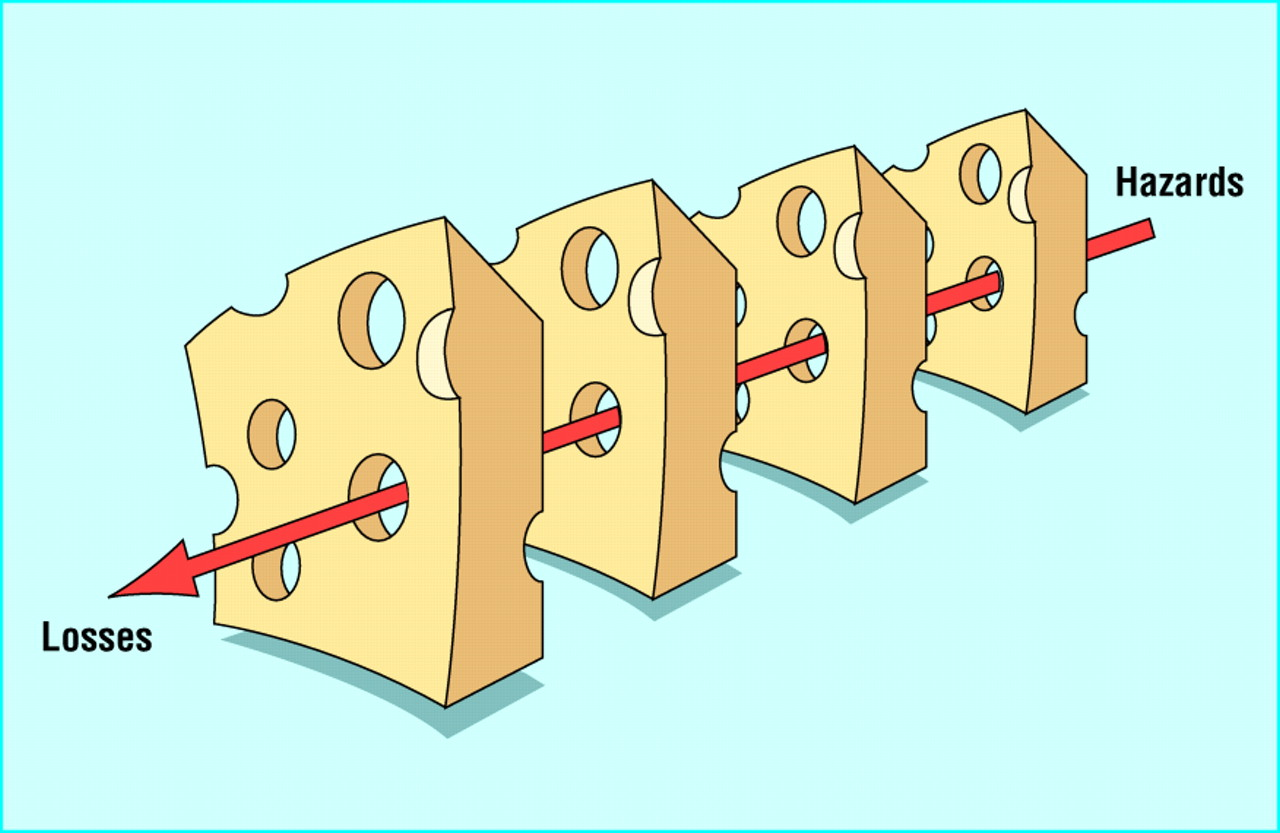
\includegraphics[width=0.8\textwidth]{fig/innledning/sveitserost.jpg}
    \caption{Sveitserostmodellen viser hvordan feil kan skje tross flere lag med sikringstiltak     \citep{HumanErrorModelsManagement}.}
    \label{fig:sveitserost}
\end{figure}

I helsevesenet finnes det mange prosedyrer, protokoller, helsepersonell og utstyr som er ment å forhindre at feil oppstår. Sveitserostmodellen \citep{HumanErrorModelsManagement} vist i figur~\ref{fig:sveitserost} illustrerer hvordan ulike sikkerhetstiltak vanligvis hindrer at en feil fører til pasientskade. Problemet er at alle sikkerhetstiltakene har begrensninger, eller “hull”. En trussel kan dermed passere alle sikkerhetstiltakene i noen tilfeller.  

Når feil skjer i legemiddelhåndteringsprosessen er det pasienten som blir skadelidende. Innsikt i egen legemiddelsituasjon kan gi pasienten bedre forutsetninger for å kontrollere at legemiddelbehandlingen er optimal. 

\subsection*{Dårlig samstemming av legemiddellister}
Bruk av legemidler er et viktig tiltak i helsevesenet, men er ofte lite koordinert og ikke underlagt samlet kontroll. Ulike institusjoner har hver sine lister over hvilke legemidler pasientene står på. Det er påvist at disse listene ofte ikke stemmer overens \citep{vetFast}. 

Internasjonalt blir 25\% av reseptpliktige legemidler pasientene bruker ikke registrert ved innleggelse på sykehus \citep{BCP:BCP204}. Den manglende informasjonen om pasientens legemidler fører til feilbehandlinger og uønskede legemiddelreaksjoner \citep{doi:10.1001/jama.1995.03530010049034}. 

Pasientsikkerhetsprogrammet “I trygge hender” har et mål om å bidra til bedre samstemming av den enkelte pasient sin legemiddelliste. Deres forslag til løsning er at pasienter skal bære med seg en papirutgave av legemiddellisten \citep{Pasientsikkerhetsprosjektet}. Pasientsikkerhetsprogrammet satser på en ikke-elektronisk løsning, i motsetning til andre studier som tilsier at en elektronisk løsning kanskje ville vært bedre \citep{komLegemidler}. En elektronisk oversikt er lettere å holde oppdatert og dele. 

Oversikt over egen legemiddelsituasjon kan føre til at feil som skyldes dårlig samstemming forhindres fordi pasienten har en oppdatert legemiddelliste som kan brukes i kontakt med helsevesenet.

\subsection*{Etterlevelse}
Etterlevelse er et begrep som brukes for å beskrive om legemidler tas som forskrevet. Dårlig etterlevelse er et globalt helseproblem som hindrer pasienter i å få optimal legemiddelbehandling \citep{ConcordanceAdherenceCompliance}. Dårlig etterlevelse medfører dårligere resultat av behandlinger, og økte kostnader for helsevesenet \citep{WHO}. 

Det finnes mange årsaker til dårlig etterlevelse. En årsak er frykt for bivirkninger. I følge apotekforeningen velger 1 av 3 pasienter i Norge å ikke ta legemidlene sine i frykt for bivirkninger \citep{ApotekINorge}. Bedre informasjon om legemidler, som er lettere tilgjengelig, kan bidra til å øke pasientenes etterlevelse \citep{Donovan1992507, doi:10.1056/NEJMra050100}.  

\subsection*{Pasienter som tar flere legemidler}
Antall pasienter med flere kroniske sykdommer\footnote{Kroniske sykdommer: sykdommer med et langtrukkent forløp. Mange kroniske sykdommer er livsvarige, men andre er fullt helbredelige på lang sikt}, og som derfor tar flere legemidler fast, er økende \citep{MultimorbidityPrimaryCare}. Ved bruk av flere legemidler samtidig minker sannsynligheten for god etterlevelse \citep{JOCN:JOCN1477}. 

Pasienter som tar mange legemidler synes ofte det er vanskelig å holde rede på hvorfor de bruker de ulike legemidlene, og når legemidlene skal tas. Antall diagnoser øker med alderen, og eldre pasienter har større vanskeligheter med å oppfatte informasjon og brukerveiledninger \citep{ConcordanceAdherenceCompliance}. 

\section{Forskningsspørsmål} \label{sec:forskningssporsmaal}
Oppgavens bidrag til å nå målet var å gjennomføre et eksperiment som skulle besvare følgende forskningsspørsmål:
\thesisRQ 

Vi utviklet en prototype av et interaktivt system som inneholdt en visuell fremstilling av personlig legemiddelinformasjon. Som vist i figur~\ref{fig:prosess2} var formålet med å utvikle prototypen å bruke den i et eksperiment for å besvare forskningsspørsmålet. I eksperimentet ble prototypen sammenlignet med pakningsvedlegg. Vi valgte å sammenligne med pakningsvedlegg fordi det er en av få eksisterende kilder til legemiddelinformasjon som er rettet mot pasienter. 

\begin{figure}[H]
    \centering
    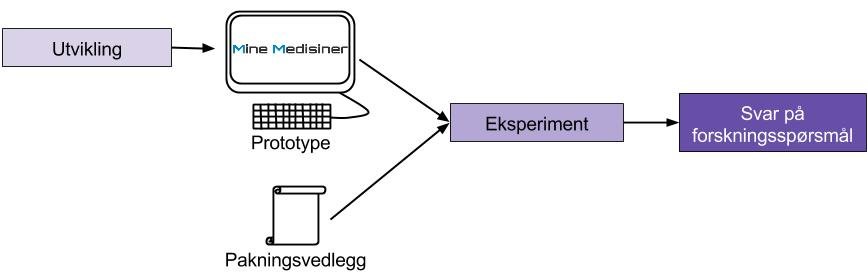
\includegraphics[width=\textwidth]{fig/innledning/prosess.jpg}
    \caption{Arbeidsprosessen mot å besvare forskningsspørsmålet}
    \label{fig:prosess2}
\end{figure}

Basert på forskningsspørsmålet utviklet vi følgende hypoteser:
\begin{enumerate}
 \item Ved å bruke prototypen får pasienter raskere svar på spesifikke spørsmål enn ved å bruke pakningsvedlegg.
 \item Ved å bruke prototypen oppfatter pasienter svaret på spesifikke spørsmål mer korrekt enn ved å bruke pakningsvedlegg.
 \item Ved å bruke pakningsvedlegg tilegner pasienter seg kunnskap utover det de leter etter, i større grad enn ved å bruke prototypen. 
\end{enumerate}


\section{Begrensninger}
I dette delkapittelet presenteres begrensingene til forskningsspørsmålet.

\subsection{Målgruppe} \label{subsec:maalgruppe}
Oppgaven er begrenset til å besvare forskningsspørsmålet for følgende målgruppe:
\begin{quote}Pasienter som tar mer enn ett legemiddel om dagen, og som bruker datamaskin på jevnlig basis.\end{quote}

\subsection{Prototype}
Bruk av et ferdig utviklet system i eksperimentet kunne ført til mer nyttige tilbakemeldinger enn en prototype med mange forenklinger. Programvareutvikling er tidkrevende og var ikke direkte nødvendig for å svare på forskningsspørsmålet. Vi valgte derfor å utvikle en prototype. Prototypen ble utviklet for å fungere for et lite utvalg brukere jf. delkapittel~\ref{sec:personae}. 

\subsection{Personvern}
Vi valgte å avgrense utviklingen av prototypen til å ikke omfatte lagring eller overføring av reelle persondata. Dette ble gjort ved at prototypen kun inneholdt data om de personae som er presentert i oppgaven. Siden prototypen ikke medførte lagring eller overføring av personlige data kunne vi se bort i fra problemstillinger knyttet til personvern. Det er viktig at en ferdig versjon av systemet tar hensyn til problemstillinger knyttet til personvern. Det er en rekke lover, regler og forskrifter som regulerer behandlingen av helseopplysninger, se delkapittel~\ref{sec:sikkerhet}. 

\section{Oppbygging av rapporten}
%\textbf{Kapittel~\ref{chap:innledning}, Innledning:} innholder en gjennomgang av motivasjonen bak oppgaven, samt forskningsspørsmål og begrensninger. Et eksempel på bruk av Mine Medisiner er også presentert. 

\textbf{\autoref{chap:bakgrunn_helsefaglig}, \nameref{chap:bakgrunn_helsefaglig}:} gir utdypning av begrepene interaksjon og bivirkning. 

\textbf{\autoref{chap:bakgrunn}, \nameref{chap:bakgrunn}:} er en gjennomgang av nødvendig bakgrunnsinformasjon om brukergrensesnitt og brukersentrert utvikling. 

\textbf{\autoref{chap:dagensSituasjon}, \nameref{chap:dagensSituasjon}:} presenterer dagens situasjon knyttet til pasienters innsyn i informasjon om egen legemiddelbruk. 

\textbf{\autoref{chap:eksperimentdesign}, \nameref{chap:eksperimentdesign}:} presenterer eksperimentdesignet for oppgaven i form av en overordnet forskningsplan.

\textbf{\autoref{chap:lit}, \nameref{chap:lit}:} er en gjennomgang av relevant litteratur knyttet til problemområdet for oppgaven.

\textbf{\autoref{chap:utviklingsmetoder}, \nameref{chap:utviklingsmetoder}:} beskriver metodene benyttet for å utvikle den digitale prototypen.

\textbf{\autoref{chap:utvikleprototype}, \nameref{chap:utvikleprototype}:} beskriver arbeidet frem mot den digitale prototypen.

\textbf{\autoref{chap:gjennomforing}, \nameref{chap:gjennomforing}:} gir en beskrivelse av forsøket som ble gjennomført for å sammenligne den digitale prototypen og pakningsvedlegg. 

\textbf{\autoref{chap:resultat}, \nameref{chap:resultat}:} presenterer resultatene fra forsøket i form av rådata og tall.
 
\textbf{\autoref{chap:analyse}, \nameref{chap:analyse}:} inneholder påstander som underbygges med resultatene fra forsøket.

\textbf{\autoref{chap:diskusjon}, \nameref{chap:diskusjon}:} inneholder diskusjon av valgene som er tatt, utfordringer som har oppstått underveis og gyldighetene av resultatene.

\textbf{\autoref{chap:konklusjon}, \nameref{chap:konklusjon}:} oppsummerer prosjektet og besvarer forskningsspørsmålet. 

\textbf{\autoref{chap:videreArbeid}, \nameref{chap:videreArbeid}:} inneholder forslag til videre arbeid.

\chapter{Legemidler} \label{chap:bakgrunn_helsefaglig}
Legemidler kan ha flere effekter. Et legemiddel har ønsket effekt hvis det har antatt virkning. En ønsket effekt for et legemiddel kan for eksempel være å kurere hodepine. Effekter kan også være negative, og inkluderer bivirkninger og interaksjoner.

Dette kapittelet vil gi en kort introduksjon til begrepene interaksjon og bivirkning som er nødvendig for å forstå forskningsspørsmålet, jf. delkapittel~\ref{sec:forskningssporsmaal}.

\section{Interaksjoner}
En interaksjon er at legemidler, legemidler og helsekostprodukter, legemidler og mat, eller legemidler og drikke, påvirker hverandre \citep{Stockley}. Interaksjoner er delt i to hovedtyper: Farmakokinetiske og farmakodynamiske interaksjoner. 

Farmakokinetiske interaksjoner betyr at et legemiddel forandrer effekten til et annet legemiddel slik at konsentrasjonen av virkestoffet i kroppen endres. Disse interaksjonene kan endre kroppens evne til opptak av legemiddelets virkestoff, distribusjonen av legemiddelet, nyttiggjøring av virkestoffet og eliminering av avfall. 

Farmakodynamiske interaksjoner forekommer når et legemiddel påvirker effekten av et annet legemiddel uten å endre konsentrasjonen i kroppen. Farmakodynamiske interaksjoner kan ha følgende effekter:
\begin{itemize}
\item \textbf{Additiv effekt} vil si at totaleffekten av flere legemidler er lik summen av effekten av de enkelte legemidlene. Dette er den mest vanlige effekten av å ta flere legemidler sammen. 
\item \textbf{Synergisk effekt} oppstår når totaleffekten av å ta flere legemidler er større enn summen av effekten av de enkelte legemidlene. 
\item \textbf{Antagonistisk effekt} oppstår når effekten av ett eller flere legemiddel blir redusert av et annet legemiddel.
\end{itemize}

\section{Bivirkninger}
Bivirkninger er alle ikke-tilsiktede effekter et legemiddel kan ha. De fleste bivirkninger er uønskede. Smerter, ubehag eller andre symptomer som oppstår ved bruk av legemidler kan være bivirkninger. Noen ganger kan det være vanskelig å avgjøre om symptomer skyldes bivirkninger, eller om de skyldes sykdom eller andre forhold.

Noen bivirkninger er forbigående, mens andre kan være alvorlige og i noen tillfeller også livstruende. Hvilke bivirkninger som er farlig er avhengig av sykdomsbildet til pasienten, hvilke legemidler pasienten tar og situasjonen for øvrig. 

Alle legemidler kan gi bivirkninger, men ikke alle som tar legemidler får bivirkninger. Det er vanskelig å forutsi hvilke pasienter som vil få bivirkninger. Eldre er mer utsatt for mange typer bivirkninger \citep{AdverseDrugReactions}.

Ikke alle bivirkninger av legemidler er kjent. Derfor er det nyttig at pasienter rapporterer bivirkninger de opplever ved bruk av legemidler. Bivirkninger kan rapporteres til Legemiddelverket via et meldeskjema\footnote{Legemiddelverkets meldeskjema for bivirkninger: \url{http://www.legemiddelverket.no/Bivirkninger/Meld_bivirkninger/Sider/default.aspx}}, eller ved å fortelle legen om dem.

Bivirkninger forekommer med ulik hyppighet. En bivirkning kalles:
\begin{itemize}
\item \textbf{svært vanlig} hvis den forekommer hos mer enn 1 av 10 pasienter,
\item \textbf{vanlig} hvis den forekommer hos mellom 1 av 10 og 1 av 100 pasienter,
\item \textbf{mindre vanlig} hvis den forekommer hos mellom 1 av 100 og 1 av 1\,000 pasienter,
\item \textbf{sjelden} hvis den forekommer hos mellom 1 av 1\,000 og 1 av 10\,000 pasienter,
\item \textbf{svært sjelden} hvis forekommer hos færre enn 1 av 10\,000.
\end{itemize}
 
\chapter{Brukergrensesnitt og brukersentrert utvikling} \label{chap:bakgrunn}
Dette kapittelet presenterer bakgrunnsteori om brukergrensesnitt og brukersentrert utvikling. 

\section{Brukergrensesnitt}

I dette delkapittelet presenteres brukbarhet, universell utforming og dialogprinsipper for interaktive systemer. Dette er viktig konsepter for å oppnå gode brukergrensesnitt. 

\subsection{Brukbarhet}
I \acrshort{iso} 9241-11 \citep{ISO9241-11} er brukbarhet definert som anvendbarhet, effektivitet og tilfredsstillelse for bestemte brukere med bestemte mål i bestemte omgivelser.
\begin{itemize}
\item Anvendbarhet er i hvilken grad brukeren klarer å utføre forhåndsdefinerte oppgaver, og oppnå forhåndsdefinerte mål.
\item Effektivitet er hvor effektiv brukeren er til å utføre forhåndsdefinerte oppgaver.
\item Tilfredsstillelse er brukerens opplevelse av systemet, den opplevde brukskvaliteten.
\end{itemize}

Anvendbarheten, effektiviteten og tilfredsstillelsen kan ikke evalueres isolert. Det må måles for de brukerne som er ment å bruke systemet, for de oppgavene systemet er ment å løse og i de omgivelsene systemet er ment i. 

Anvendbarhet og effektivitet kan enkelt måles ved telling. Anvendbarheten måles ved at man regner ut hvor mange prosent av de forhåndsdefinerte oppgavene brukeren klarte å utføre. Effektivitet kan måles ved å ta tiden på utføring av forhåndsdefinerte oppgaver.

Tilfredsstillelse er vanskeligere å måle. Standardiserte spørreskjema kan benyttes, men følelser er generelt vanskelig å representere i et spørreskjema.

\subsection{Universell utforming}
En utfordring ved utvikling av grensesnitt er at folk er forskjellige når det kommer til motivasjon, evner, bakgrunn, personlighet, alder og kjønn. Målet med universell utforming er å utvikle grensesnitt som ivaretar behovene til alle brukere.

Ved utvikling av universelt design bør man passe på å ikke lage et “minste felles multiplum” eller en “fordumming” av systemet som gjør det mindre nyttig for mange brukere \citep{MMIboken25}. Det er viktig å legge til rette for bruk av dårlig teknologi \footnote{Dårlig teknologi: for eksempel må det legges til rette for å kunne bruke gamle/trege datamaskiner}, brukere med lite teknisk erfaring og brukere med funksjonshemninger. Man må imidlertid også påse at systemet fungerer bra for andre brukere.

Ved utvikling av grensesnittet til et system som er laget for pasienter som tar flere legemidler fast bør det tas spesielle hensyn, blant annet fordi denne brukergruppen består av mange eldre. Når folk blir eldre skjer det forandringer i deres funksjonelle ferdigheter. Oppfattelsesevne, responshastighet og kognitive evner reduseres. Det er individuelle forskjeller i hvor fort disse forandringene skjer \citep{designForGamlisser}. 

Brukergrensesnitt kan bli mer brukervennlig for eldre dersom brukerne får kontroll over fontstørrelse, fargekontraster og lydvolum. Bedre pekeenheter, tydeligere navigasjonsstier og konsekvent layout kan også bidra til at brukergrensesnitt blir mer brukervennlig. Selv om disse forbedringene gjør størst forskjell for eldre, vil de øke brukervennligheten for andre aldersgrupper \citep{designForGamlisser}.

I Norge stilles det krav om universell utforming av \acrshort{ikt}-løsninger ved lov, jf diskriminerings- og tilgjengelighetsloven §14. Loven blir presisert i forskrift om universell utforming av \acrshort{ikt}-løsninger §2 og §4\footnote{Informasjon og veiledning for forskrift om universell utforming: \url{http://uu.difi.no/}}, der kommer det frem at man må følge \acrshort{wcag} (2.0)-standarden når man lager nettsider som retter seg mot “allmennheten”. 

\subsubsection{WCAG 2.0}
\acrfull{wcag} 2.0 er en del av en serie med retningslinjer for å gjøre internett tilgjengelig for alle, uavhengig av hvilke verktøy som brukes får å navigere på nettet, eller hvilke begrensninger brukere opererer under. 

\acrshort{wcag} 2.0 er bygd opp av fire prinsipper, som er videre inndelt i 12 retningslinjer og 61 testbare suksesskriterier. Suksesskriteriene er inndelt i tre nivåer: A, AA og AAA. Oppbyggingen er illustrert i figur~\ref{fig:wcag_tabell}.

\begin{figure}[H]
    \centering
    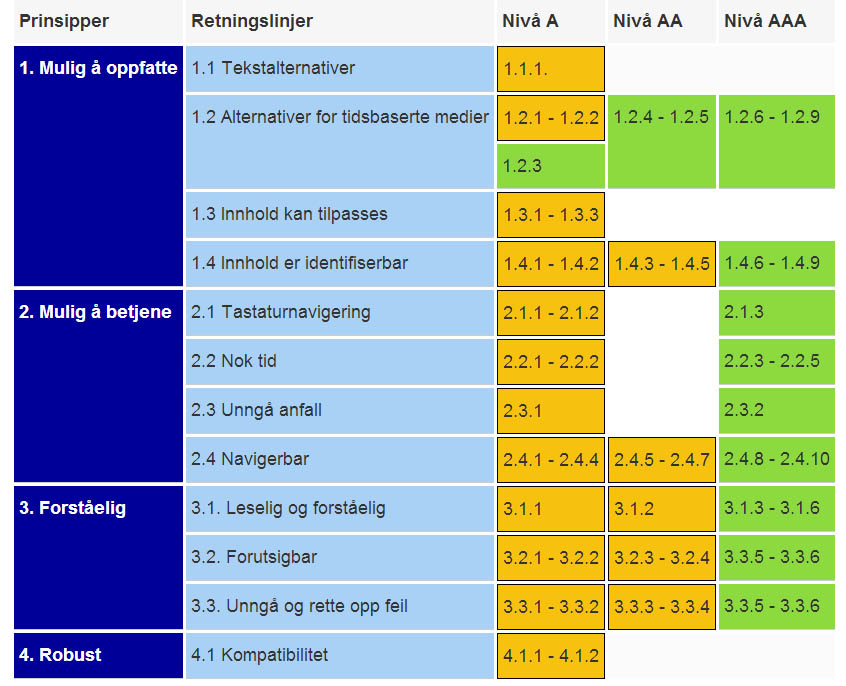
\includegraphics[width=0.9\textwidth]{fig/bakgrunn/wcag_tabell.jpg}
    \caption{Oppbygging av \acrshort{wcag} 2.0. De oransje kravene er omfattet av forskrift for universell utforming av \acrshort{ikt}-løsninger. Kilde: \url{http://uu.difi.no/veiledning/nettsider/krav-til-nettsider/oppbygging-av-wcag-20} }
    \label{fig:wcag_tabell}
\end{figure}

Forskrift om universell utforming av \acrshort{ikt}-løsninger fastslår at tilgjengelige nettsider skal lages i samsvar med nivåene A og AA, med unntak av kravene som gjelder teksting av direktesendt lyd og synstolking av innspilt video. Forskriften stiller dermed krav om at 35 av de 61 suksesskriterier skal følges.

\subsection{Dialogprinsipper}
\acrshort{iso} 9241-110:2006 "Ergonomi for samhandling mellom menneske og system - Del 110: Dialogprinsipper" beskriver 7 dialogprinsipper for interaktive systemer. En dialog defineres som en interaksjon mellom en bruker og et interaktivt system i form av brukerhandlinger og systemsvar som skal til for å oppnå et mål. Dialogprinsippene gjelder utformingen av brukergrensesnitt og skal bidra til å økt brukervennlighet for interaktive systemer. 


\section{Brukersentrert utvikling} \label{sec:brukersentrert}
Brukersentrert utvikling er en utviklingsfilosofi som handler om aktiv involvering av brukere gjennom hele utviklingsprosessen. Brukerdrevet utvikling fokuserer på å oppnå høy brukbarhet, og er mye brukt i systemutvikling. 

\acrshort{iso} 9241-210:2010 “Ergonomi for samhandling mellom menneske og system - Del 210: Menneskeorientert design for interaktive systemer” beskriver fire brukersentrerte aktiviteter som bør finne sted i brukersentrert utvikling:
\begin{enumerate}
\item Forstå og spesifisere brukskonteksten
\item Spesifisere brukernes og organisasjonens krav
\item Utvikle designløsninger
\item Evaluere design mot krav
\end{enumerate}

\begin{figure}[H]
    \centering
    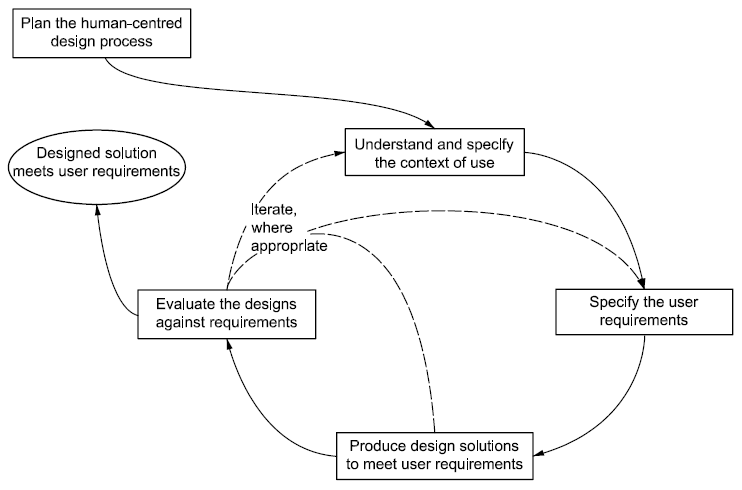
\includegraphics[width=0.8\textwidth]{fig/bakgrunn/ISO9241-210.PNG}
    \caption{Den gjensidige avhengigheten i brukersentrerte designaktiviteter, kilde: ISO 9241-210:2010 }
    \label{fig:ISO9241}
\end{figure}

Utviklingsaktivitetene inngår i en iterativ prosess der hver aktivitet kan bruke resultatene fra en annen aktivitet. Aktivitetene utføres ikke i streng rekkefølge. Standarden erkjenner at i det virkelige liv må man noen ganger gå tilbake til tidligere aktiviteter, og revurdere hva som gjøres der, etter å ha utført en aktivitet. Ulike aktiviteter kan skje samtidig. Prosessen er illustrert i figur~\ref{fig:ISO9241}.

Brukerdrevet utvikling kan være kostbart i form av at det er tidkrevende, men vil kunne være kostnadsbesparende på sikt ved at brukernes behov blir kartlagt underveis i utviklingsprosessen. Involvering av brukere i utviklingsprosessen er en verdifull kilde til informasjon om brukskontekst og oppgavene systemet skal løse \citep{usercentereddesign}.


\section{Prototyping} \label{sec:prototyping}
Prototyping er mye brukt i brukersentrert utvikling. Prototyping er prosessen som benyttes for å lage prototyper av systemer. En prototype er en foreløpig utgave av et system som lages før selve systemet settes i produksjon. Prototyper brukes til å demonstrere konsepter, teste designmuligheter og få innsikt i problemer og mulige løsninger \citep{suBoken}.

\begin{figure}[H]
    \centering
    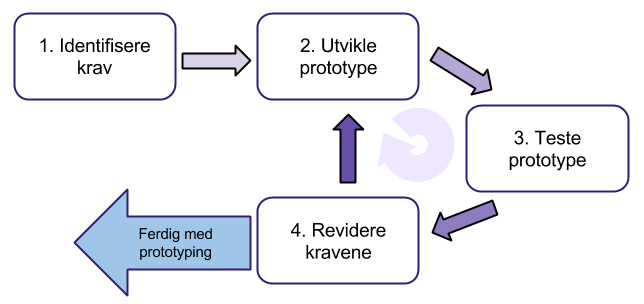
\includegraphics[width=1\textwidth]{fig/bakgrunn/prototype.png}
    \caption{Trinnene i prototypingsprosessen}
    \label{fig:prototype}
\end{figure}

Figur~\ref{fig:prototype} illustrerer prototypingsprosessen. Prosessen består av en rekke trinn som gjennomføres iterativt, der resultatet av en prototypetest danner grunnlaget når en ny prototype utvikles:
\begin{enumerate}
\item \textbf{Identifisere krav:} I det første trinnet identifiseres initielle krav og spesifikasjonene for systemet.
\item \textbf{Utvikle Prototype:} En prototype blir utviklet basert på kravene og spesifikasjonene som er identifisert.
\item \textbf{Teste prototype:} Den ferdige prototypen evalueres gjennom en prototypetest med brukere.
\item \textbf{Revidere kravene:} Kravene og spesifikasjonene for systemet blir revidert basert på tilbakemeldingene som er mottatt i prototypetesten. Hvis prototypeprosessen ikke er avsluttet etter dette trinnet, blir trinn 2-4 gjentatt. En ny prototype blir da utviklet, enten fra bunnen av eller som en forbedret versjon av den gamle prototypen.
\end{enumerate}

Før en prototype utvikles blir det tatt beslutninger om hvilken funksjonelle krav som skal inkluderes. For å minimere tiden det tar å lage prototypen er det bare den viktigste funksjonaliteten som blir inkludert\citep{suBoken}. En prototype er en forenklet versjon av det endelige systemet. Ved å teste et endelig system kan man få bedre tilbakemeldinger, men det er mer krevende. Prototyping gjør det mulig å få verdifulle tilbakemeldinger tidlig i utviklingsprosessen. Når endringer i kravspesifikasjon eller design oppdages tidlig krever det mindre arbeid å implementere endringene.

Det finnes mange typer prototyper, for eksempel papirbaserte prototyper og klikkbare digitale prototyper. Papirbaserte prototyper er skisser av et system, laget for hånd eller ved hjelp av digitale verktøy. Papirversjoner av elektroniske systemer kan være vanskelig å forstå for brukere, noe som kan føre til at tilbakemeldingene ved testing av funksjonalitet blir mindre verdifulle. 
En klikkbar digital prototype ligner mer på et ferdig system enn en papirprototype, da noe brukerinteraksjon er mulig ved hjelp av museklikk og tastetrykk. 

Papirbaserte prototyper har den fordel at de er raske og enkle å lage. Ifølge \citep{prototypingWebDesign} har papirprototyper også en fordel ved at brukere er mer komfortabel med å komme med tilbakemeldinger og kritikk av papirprototyper enn digitale prototyper. De begrunner dette med at papirprototyper virker mindre ``ferdig'' og ``ekte'' enn digitale prototyper, og at det fremstår som mindre arbeidskrevende å implementere foreslåtte endringer.



    
\chapter{Dagens situasjon} \label{chap:dagensSituasjon}
Dette kapittelet presenteres dagens situasjon knyttet til pasienters innsyn i informasjon om egen legemiddelbruk. Først presenteres legemiddelhåndteringsprosessen, og svakhetene ved den som gjør at pasienter kan ønske å ha innsyn i egen legemiddelsituasjon. Deretter presenteres hvilken rett pasienter har til innsyn i opplysninger lagret i egen journal, og hvordan pasienter kan få tilgang til disse opplysningene. Så presenteres kilder til legemiddelinformasjon som pasienter har tilgang til i dag, og pasientkontrollerte systemer som er er utviklet av store internasjonale selskaper, men som ikke er tatt i bruk i Norge. Til slutt presenteres lover og regler som skal sikte at personvernet er ivaretatt av personlige legemiddelinformasjonskilder.
 
\section{Legemiddelhåndteringsprosessen}
Dette delkapittelet beskriver de ulike aktivitetene som inngår i legemiddelhåndteringen, og informasjonsoverføringen som skjer mellom hver aktivitet. Legemiddelhåndtering beskriver legemiddelrelaterte oppgaver i en kjede av trinn fra legen beslutter bruk av et legemiddel til det er brukt av pasienten. I dette kapittelet er det valgt å dele inn legemiddelhåndteringsprosessen i følgende underaktiviteter: Ordinering, utlevering, dosering og inntak av dose, se figur~\ref{fig:prosess}.

\begin{figure}[h]
    \centering
    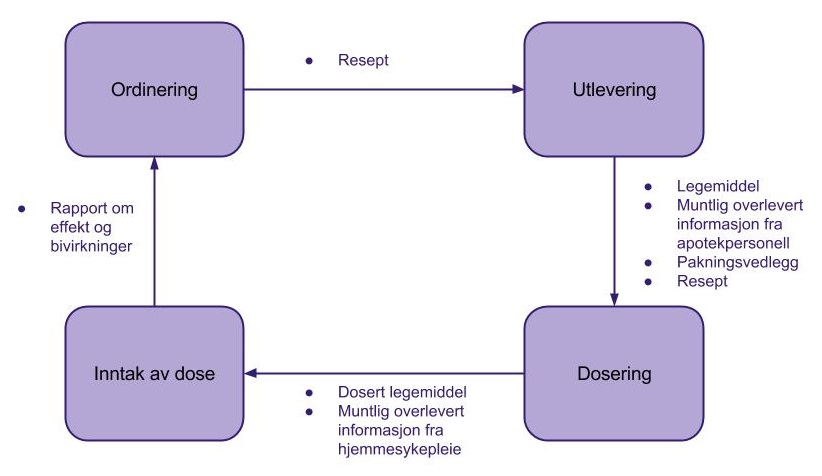
\includegraphics[width=0.9\textwidth]{fig/dagens/prosess.jpg}
    \caption{Aktivitetene ved legemiddelhåndtering og informasjonsoverføringen som finner sted mellom aktivitetene}
    \label{fig:prosess}
\end{figure}

\subsection{Ordinering}
Ordinering er at legen bestemmer bruk av legemiddel og dosering, og journalfører dette, jf. forskrift om legemiddelhåndtering § 3 bokstav g. Først har legen foretatt en medisinskfaglig vurdering, og funnet ut at pasienten trenger behandling med et eller flere legemidler. Legemidlene som ordineres er et ledd i en behandling hvor legen må passe på å angi riktig legemiddel og dosering. Legen skal kontrollere at ordineringen er forsvarlig med tanke på interaksjoner med andre legemidler i bruk, allergier og pasientens tilstand generelt. Legen skal skaffe oversikt over pasientens helsesituasjon gjennom direkte kontakt med pasienten og kommunikasjon med annet helsepersonell, jf. st. meld nr. 18 (2004-2005).
 
Etter en ordinering blir det gjort en rekvirering. Rekvirering er definert som en “muntlig, skriftlig eller elektronisk bestilling av legemiddel ved resept eller rekvisisjon”, jf. forskrift om legemidler fra apotek § 1-3 bokstav e og forskrift om legemiddelhåndtering § 3 bokstav f. Det vanligste er at bestillingen blir opprettet som en elektronisk resept (eResept). Bestillingen som opprettes ved rekvirering er en del av informasjonsutvekslingen fra ordineringsfasen til utleveringsfasen.
 
Ifølge helsepersonelloven § 11 kan leger rekvirere reseptbelagte legemidler. De fleste rekvireringer av legemidler gjøres av fastlegen, men mange rekvireringer skjer også av leger i spesialisthelsetjenesten \citep{stmeld1820042005}.Det at flere leger rekvirerer legemidler til den samme pasienten kan gjøre det vanskelig for legene å holde oversikt over hvilke legemidler pasienten står på. 

Fastlegeordningen ble innført i Norge i 2001, og skal sikre at alle som ønsker det har én bestemt allmennlege å forholde seg til. I følge forskrift om fastlegeordning i kommunene § 10 er en fastlege i utgangspunktet ansvarlig for å tilby alle typer “allmennlegeoppgaver” for innbyggerne på sin liste.  Det er vanskelig å avgjøre hva som er “allmennlegeoppgaver” da ordlyden er vid og uklar. Dette gjør at det er vanskelig å avklare nøyaktig hva som er fastlegens ansvar knyttet til sine pasienters legemiddelbruk. 

Forskrift om fastlegeordning i kommunene § 25 kan bidra til å få klarhet i dette. Ifølge forskriften skal fastlegen “koordinere” legemiddelbehandlingen til innbyggerne på sin liste. Dette innebærer å oppdatere legemiddellisten til pasienten når fastlegen endrer eller får informasjon om at legemiddelbehandlingen er endret. For at fastlegen skal kunne oppdatere legemiddellisten er det altså viktig at informasjon om endringer av andre blir formidlet til fastlegen. Pasienter har ofte feil legemiddellister på grunn av dårlig informasjonsutveksling mellom ulike aktører eller fordi informasjon som blir utvekslet ikke blir fulgt opp. Sykehusepikrisen fungerer ofte som eneste form for informasjonsoverføring fra spesialisthelsetjenesten til fastlegene. En undersøkelse gjort i Tromsø \citep{komLegemidler} i 2007 viste at mange epikriser kom frem svært sent (noen ganger ble ikke epikrisen sendt ut i det hele tatt) og det var bare tre av ni leger som oppdaterte legemiddellisten når de mottok epikrise fra sykehusene.

Det følger av forskrift om fastlegeordning i kommunene § 14 at dersom en person som står på fastlegens liste blir inntatt i en helse- og omsorgsinstitusjon eller annen institusjon med organisert legetjeneste, overføres legemiddellisteansvaret etter forskriftens § 10 til institusjonen. Mens pasienten er på institusjon har altså ikke fastlegen lenger ansvar fordi institusjonen overtar det ansvaret fastlegen tidligere hadde. For å kunne overta ansvaret på en god måte trenger institusjonen informasjon fra fastlegen om pasientens legemiddelliste. Det er ikke alltid denne informasjonsoverføringen fungerer optimalt. Særlig legevakten har hatt problemer med at de ikke mottar nødvendige opplysninger om legemiddelbruk \citep{komLegemidler}. 

\subsection{Legemiddelgjennomgang} \label{subsec:legemiddelgjennomgang} 
Legemidler brukes ofte ikke slik de er tiltenkt, noe som kan føre til legemiddelrelaterte problemer\footnote{Legemiddelrelatert problem: “en hendelse eller et forhold som skjer i forbindelse med legemiddelbehandling og som reelt eller potensielt interfererer med ønsket helseeffekt”\citep{legemiddelgjennomgang}} \citep{WHO}. Mange av disse problemene kan enkelt forebygges. Et av tiltakene som er iverksatt for å begrense og forebygge legemiddelrelaterte problemer er at leger skal gjennomføre legemiddelgjennomgang av pasientenes legemidler. 

En legemiddelgjennomgang er en “strukturert/systematisk evaluering av den enkelte pasientens legemiddelregime i den hensikt å optimalisere effekten av legemidlene og redusere risiko ved legemiddelbruk” \citep{legemiddelgjennomgang}. En legemiddelgjennomgang kan resultere i at at pasientens legemiddelliste endres.

Legemiddelgjennomgang kan gjøres av behandlende lege alene eller sammen med sykepleiere, farmasøyter eller pasienten det gjelder. Behandlende lege er ansvarlig for beslutninger fattet i forbindelse med legemiddelbehandling av pasienter. Derfor er behandlende lege ansvarlig for de endelige beslutningene tatt i legemiddelgjennomgangen.

Før det kan gjøres en legemiddelgjennomgang må det gjøres en legemiddelsamstemming. En legemiddelsamstemming vil si at det lages en korrekt liste over alle legemidlene en pasient bruker. Listen som utarbeides i samstemmingsprosessen kalles “Legemidler i bruk” (\acrshort{lib}). Informasjonen som trengs for å lage listen hentes blant annet fra e-resepter, pasientjournaler og pasientens egen liste \citep{sjekklisteLegemiddelgjennomgang}.
 
En legemiddelgjennomgang skal utføres ved endring i situasjon, eller regelmessig dersom pasienten tar minst fire legemidler, jf. Forskrift om fastlegeordning i kommunene § 25. I følge forskriften er det fastlegen som er ansvarlig for at en slik legemiddelgjennomgang blir gjennomført.
 
Legemiddelverket har lansert en sjekkliste\footnote{Les mer om legemiddelverkets sjekkliste for legemiddelgjennomgang her:\url{http://www.kunnskapssenteret.no/verktoy/sjekkliste-for-legemiddelgjennomgang}} for legemiddelgjennomgang. Det er en kortfattet veiledning som inneholder sjekkpunkter og en liste med legemidler man bør være spesielt oppmerksomme på. Sjekklisten bygger blant annet på \acrshort{start}/\acrshort{stopp}-kriteriene og \acrshort{norgep}. Mer om legemiddelgjennomgang i delkapittel~\ref{sec:littLegemiddelgjennomgang}.

\subsubsection{Start Stopp NorGeP}
De fleste legemidler har bivirkninger, og det er derfor ønskelig at pasienter ikke tar flere legemidler enn nødvendig. Det er derfor publisert tre verktøy som skal hjelpe legen med å vurdere om alle pasientens legemidler er nødvendige, og om pasienten får alle nødvendige legemidler. De tre verktøyene heter: \acrshort{start}, \acrshort{stopp} og \acrshort{norgep}. 

\acrshort{start} og \acrshort{stopp} er utviklet i Irland. De har blitt oversatt til norsk med noen justeringer for at de skal samsvare med norsk terapitradisjon. I 2015 ble \acrshort{start} og \acrshort{stopp} oppdatert med ny informasjon. De nye versjonene heter START2 og STOPP2. \acrshort{norgep} er utviklet i Norge. 

\acrshort{start}, \acrshort{stopp} og \acrshort{norgep} har særlig fokus på eldre. Mange eldre mennesker får legemidler for flere lidelser, og er spesielt utsatt for uheldige effekter av legemiddelbehandling. Forandringer som skjer i kroppen grunnet høy alder gjøre at farmodynamikken endrer seg.

\acrshort{start}\footnote{Les mer om START her: \url{http://legemiddelhandboka.no/Generelle/311103}}(\acrlong{start}) er et hjelpemiddel for å sjekke at pasienter får de anbefalte legemidlene ved lidelser som ofte ikke behandles tilstrekkelig hos eldre.
 
\acrshort{stopp}\footnote{Les mer om STOPP her: \url{http://legemiddelhandboka.no/Generelle/315753}}(\acrlong{stopp}) er et hjelpemiddel som skal synliggjøre potensielle uhensiktsmessige legemidler. Stopp er egnet for både allmennpraksis og sykehus.

\acrshort{norgep}\footnote{Les mer om NorGeP her: \url{http://legemiddelhandboka.no/Generelle/311393}}(\acrlong{norgep}) inneholder en relevant liste av legemidler, legemiddeldoser, og legemiddelkombinasjoner som bør unngås av eldre over 70 år. 

\subsubsection{Resept}
Resept er definert som en bestilling av et legemiddel, jf. forskrift om legemidler fra apotek §1-3 bokstav c. En repsept er er en del av informasjonsflyten fra ordineringsfasen til utleveringsfasen. Fra og med tidlig 2013 er de fleste resepter i Norge elektroniske. Det finnes ulike typer resepter. Forskjellen mellom disse er forklart i de to neste avsnittene.

Legemidler som er klassifisert som sterke narkotiske stoffer må rekvireres på en spesialblankett som kalles narkotikaresept eller A-resept. Hvis legemiddelet som rekvireres er klassifisert som et vanedannende legemiddel omtales resepten gjerne som B-resept. C-resept er for alle reseptpliktige legemidler som ikke omfattes av A- eller B-resept.

Blå resept skrives ut når pasienten har krav på å få dekket deler av legemiddelutgiftene av staten. For legemidler rekvirert på hvit resept må utgifter dekkes av pasienten. 

\subsection{Utlevering}
I Norge har apotekene enerett til å selge og utlevere legemidler, jf. legemiddelloven § 16 andre ledd. Forarbeidene\footnote{Ot.prp. nr. 29 (1998-99)} forklarer at denne eneretten skal bidra til å sikre at legemidlene har god kvalitet og at de blir riktig oppbevart. Apotekene har leveringsplikt for alle legemidler, og skal sørge for at legemidler og viktig medisinsk utstyr er tilgjengelig \citep{apotekOgLegemidler2013}.
 
Apotekene er kompetansebedrifter som skal bidra til riktig og rasjonell legemiddelbruk. De skal hindre feilbruk og uheldig overforbruk av legemidler gjennom veiledning og farmasøytiske tjeneste. Det følger av forskrift\footnote{Forskrift om legemidler fra apotek § 8-2}, at apotekene skal bidra til at den som mottar legemidler har “tilstrekkelige” opplysninger om legemidlet til at det kan brukes riktig.

På apotek jobber farmasøyter og apotekteknikere. Titlene farmasøyt og apotekteknikker kan bare benyttes i Norge om personer som er autorisert etter helsepersonelloven. Farmasøyter som jobber på apotek har ansvar for å utlevere legemidlene til pasienten, kontrollere resepten og veilede om bruk. Apotekteknikerne har kontakt med kundene på apoteket og bistår farmasøytene.
 
Tradisjonelt har farmasøytrollen bare vært knyttet til legemiddelet som produkt, og ekspedering av legemidler. Det fokuseres nå også på oppgaven å gi informasjon om riktig legemiddelbruk, samt bidra til å avdekke og forebygge legemiddelrelaterte problemer. Det er imidlertid ikke helt klart hvor langt denne oppgaven strekker seg, og hva apotekets informasjonsplikt innebærer. Helse og omsorgsdepartementet påpeker i forarbeidene til apotekloven\footnote{Ot.prp. nr. 29 (1998-99)} at ansvaret for legemiddelinformasjon knyttet til behandling alltid påhviler legen. Det er derfor viktig at apoteket ikke gir informasjon som strider mot det legen har bestemt. For legemidler som ikke er reseptpliktige stiller saken seg annerledes. I disse tilfellene har det ikke vært noen lege som har vurdert legemiddelbehovet. Dermed får apoteket et hovedansvar for at kunden får tilstrekkelig informasjon. For legemidler uten resept kan apoteket komme i en situasjon hvor de må gi råd om ikke-bruk eller ikke-salg.

\subsubsection{Sykehusapotekene}
Det er 30 sykehusapotek i Norge. I apotekloven §1-3 bokstav d er et sykehusapotek definer som et “apotek i samlokalisering med offentlig sykehus eller privat sykehus som inngår i offentlige helseplaner, som har legemiddelforsyning til sykehuset som sin primæroppgave”. 

Staten overtok eieransvaret for de offentlige sykehusene ved sykehusreformen som ble innført i 2002. Som følge av sykehusreformen ble sykehusapotekene en del av spesialisthelsetjenesten, de ble overført til staten og videre til de regionale helseforetakene (Helse Sør-Øst, Helse Vest, Helse Midt-Norge, Helse Nord). 

Formålet med sykehusapotekene er fastsatt av det regionale helseforetaket de tilhører, og skiller seg derfor noe fra region til region. Felles for alle sykehusapotek er at de skal sikre forsyningen av legemidler til det sykehuset apoteket er tilknyttet, være pasientenes og sykehusets kompetansesenter for legemidler og produsere de legemidler som ikke kan skaffes på annen måte, så langt det lar seg gjøre \citep{sykehusapotekenesOrganisering}. 

\subsection{Dosering}
I forskrift om legemiddelhåndtering § 3 bokstav d defineres istandgjøring av legemidler som ”Tilberedning eller annen klargjøring av legemiddel for utdeling til pasient.”. Utdeling av legemidler skjer på ulike måter avhengig av hvor pasienten er og hvilke tjenester pasienten benytter seg av. I merknadene til forskriften\footnote{Merknader til forskrift om legemiddelhåndtering for virksomheter og helsepersonell som yter helsehjelp, Til §2} står det at det ved avtale eller vedtak kan bestemmes at hjemmesykepleien har ansvaret for istandgjøring av en pasients legemidler. 

For de som bruker flere legemidler er det viktig å holde legemidler for hvert inntakstidspunkt atskilt. Ved bruk av multidose\footnote{Multidose: maskinpakket, forseglet pose som inneholder legemidlene pasienten skal ta til et bestemt tidspunkt på dagen.} kommer legemidlene ferdig pakket og merket med inntakstidspunkt. Et annet hjelpemiddel som også brukes av hjemmesykepleien for å dosere pasientenes legemidler er dosett \citep{HelsetilsynetRapport}. 

På institusjon og i hjemmesykepleien har sykepleiere eller vernepleiere ansvar for at legens ordinasjon blir fulgt. Det vil si å sørge for at rett legemiddel gis til rett pasient, i rett legemiddelform, i rett dose, på rett måte, til rett tid og med rett informasjon. Oppgaven er en delegert legeoppgave, jf. Helsepersonelloven § 5. Oppgaven innebærer også at sykepleieren har ansvar for å foreta observasjon av behandlingens effekt, og gi lege beskjed dersom noe uventet inntreffer \citep{IllustrertFarmakologi}. 

Dersom legemidlene er dosert og satt frem av én person, men gis til pasienten av en annen, er det den som gir legemidlet til pasienten som er ansvarlig for at alt er korrekt. Det er derfor viktig at den som deler ut legemiddelet sjekker at legens ordinering er fulgt \citep{IllustrertFarmakologi}. 

For at sykepleiere/vernepleiere skal kunne gi riktige legemidler er det viktig at de har tilgang til korrekt informasjon om hva legen har bestemt. I en studie i Tromsø \citep{komLegemidler} kom det frem at særlig hjemmetjenesten ikke var fornøyd med tilgangen til og kvaliteten på informasjonen om medisinering. I undersøkelsen kom det frem at resept ofte fungerte som eneste skriftlige kommunikasjon fra fastlegen til hjemmesykepleien. 

Pasienter som befinner seg utenfor helseinstitusjoner, og ikke benytter seg av hjemmesykepleie, har selv ansvar for at legemidlene tas etter legens anvisning. Legen og apoteket har et ansvar om å gi tilstrekkelig informasjon til at pasienten kan ta legemidlene riktig. 

\subsubsection{Dosett}
Dosett er en oppbevaringsbeholder for tabletter eller kapsler. Figur~\ref{fig:dosett} viser hvordan en dosett kan se ut. I en dosett sorteres legemidlene etter mengde og inntakstid. Meningen med dosett er å forenkle dosering av legemidler.

\begin{figure}[h]
    \centering
    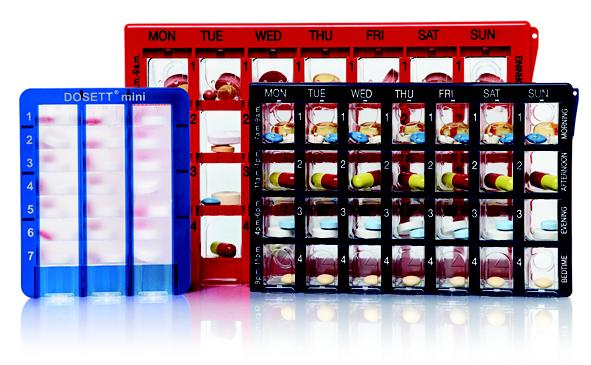
\includegraphics[width=0.6\textwidth]{fig/dagens/dosett.jpg}
    \caption{Ulike typer dosett, hentet fra: \url{http://www.dosett.com/}}
    \label{fig:dosett}
\end{figure}

\subsubsection{Multidose}
Multidose er en maskinpakket, forseglet pose som inneholder legemidlene pasienten skal ta til et bestemt tidspunkt på dagen, se Figur~\ref{fig:multidose}. Multidose er ment å være et virkemiddel for å sikre riktig legemiddelhåndtering, og forenkle hverdagen for brukere med flere medikamenter, pårørende og helsetjenesteytere \citep{OmMultidose}. Multidose brukes av pasienter med stabil legemiddelbruk, slik at legemiddellisten ikke endres fra multidosen er bestilt til alle legemidlene i multidoserullen er inntatt. 

\begin{figure}[h]
\centering
\makebox[\linewidth][c]{%
\begin{subfigure}[b]{2in}
    \centering
	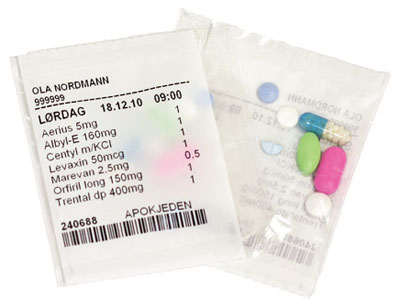
\includegraphics[width=2in]{fig/dagens/dosepakking.jpg}
	\caption{Multidosepakke}\label{fig:multidosepakke}
\end{subfigure}
\quad
\begin{subfigure}[b]{3.2in}
    \centering
    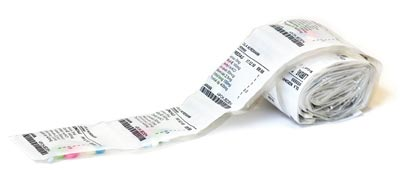
\includegraphics[width=3.2in]{fig/dagens/multidoserull.jpg}
    \caption{Multidoserull}\label{fig:multidoserull}
\end{subfigure}
}
\caption{Bilder av multidosepakninger, hentet fra: \url{http://www.apotek1.no/multidose/faa-legemidlene-dine-pakket-i-ferdige-doser}}\label{fig:multidose}
\end{figure}

Pasienter med multidose har mindre kunnskap om legemidlene de tar enn andre pasienter \citep{Kwint01092013}. På multidosepakningene finnes det kun informasjon om legemidlets navn og inntaks tidspunk, det står ikke noe om hva medisinen skal behandle. På multidosepakningen er det altså en meget begrenset mengde informasjon om legemidlene som er tilgjengelig. I tillegg står informasjonen på multidosepakkene med liten skrift, noe som gir redusert lesbarhet for brukere med dårlig syn. 

Innføring av multidose har gitt høyere etterlevelse, og ført til at legemiddellistene er bedre samenstilt mellom ulike instanser \citep{Wekre01102010}. Legemiddellistene til pasienter med multidose blir imidlertid sjeldnere revidert enn pasienter som får tradisjonell forskrivning \citep{mutiDose,Larsen2007265}. Leger opplever at justeringer av legemidler/doser er mer krevende når pasienter bruker multidose \citep{doi:10.3109/02813432.2011.554002}, og leger har ulik oppfatning om hvem som som har ansvaret for legemiddellisten til pasienter som flere leger kan rekvirere multidose til \citep{Rahmner01012010, Wekre01082012}.

Studier har vist at pasienter på multidose oftere har en uhensiktsmessig legemiddelliste, med flere potensielt farlige kombinasjoner av legemidler, enn pasienter som får vanlig ordinering \citep{23295105, PDS:PDS2232}. Det er beregnet at pasienter med multidose har 5,9 ganger høyere sjanse enn andre for å bli utsatt for feil i forbindelse med legemidler \citep{multidoseFeil}. Denne beregningen kan delvis skyldes at det er lettere å oppdage problemer hos pasienter med multidose. Multidosepakningen gir en oversikt over hvilke legemidler pasienten tar, noe som kan gjøre det lettere å se hvilke feil som eksisterer.

\subsection{Inntak av dose}
Siste aktivitet i legemiddelhåndteringen er at pasienten inntar legemiddelet.

Hjemmesykepleien eller annet pleiepersonell hjelper ofte til med å gjøre i stand dosen som skal tas. De kan klargjøre en dosett (for en hel uke), som pasienten selv må ta riktige legemidler fra, eller de kan ha klargjøre den enkelte dosen. Det er vanlig at pasienten inntar legemiddelet selv \citep{AutomatiskPilledispenser}.
 
Noen pasienter får hjelp til å innta noen typer legemidler. Det er for eksempel vanlig å få hjelp til å ta sprøyter. Dersom pasienten har kraftige funksjonshemninger kan pasienten få hjelp med inntak av legemidler på former som ellers er vanlig å ta selv. For eksempel kan en pasient som ikke har bevegelse i armene få hjelp med å føre en tablett til munnen. 

\subsubsection{Oppfølging av medisineringens effekt}
I følge \citep{HelsetilsynetRapport} foreligger det ingen retningslinjer på hvordan effekt av medisinering skal registreres, observeres og følges opp. I hjemmesykepleien er det vanlig at avdelingssykepleieren instruerer resten av personalet i hva som bør følges ekstra med på hos den enkelte pasient. Pleiepersonalet rapporterer uvanlige reaksjoner på legemidler. I hjemmesykepleien og på sykehjem blir dette ført inn i den elektroniske journalen for hver enkelt pasient. Denne journalen brukes primært av vakthavende sykepleier, og blir ikke lest på rutinebasis av legen på sykehjemmet. Fastlegen har ikke direkte tilgang til journalen til hjemmesykepleien.

\subsection{Oppsummering av legemiddelhåndteringsprosessen}
Legemiddelhåndtering er en prosesss som involverer mange aktører. Siden mange deltar i arbeidet kan det være vanskelig for den enkelte å holde oversikt over hele prosessen. Fordi det er mange prosessledd involvert i legemiddelhåndteringen er det viktig at informasjonsoverføringen mellom leddene er god, for å sikre at aktørene har tilgang på korrekt og fullstendig informasjon. Mange legemiddelskader skjer på grunn av dårlig informasjonsoverføring \citep{HelsetilsynetRapport, komLegemidler}.

Helsetilsynet beskriver legemiddelhåndteringsprosessen på følgende måte:
“Prosessen kjennetegnes av at den gjennomføres av personell som ser lite til hverandre i det daglige arbeidet, som for eksempel lege, apotek og pleiepersonale. Dette gjør den ekstra sårbar for misforståelser og feil, særlig når informasjon overføres fra et prosessledd til det neste.” \citep{HelsetilsynetRapport} 

Lover og forskrifter er uklar på hvilke aktører som har ansvar for hva, og hvor langt de ulike aktørenes ansvar strekker seg. Dette gjør det vanskelig for hver aktør å vite om de tar ansvar for det de skal, og når de beveger seg ut på andres ansvarsområde. 

Når det skjer feil i legemiddelhåndteringsprosessen som gjør at pasienten får dårligere legemiddelbehandling er det pasienten som blir skadelidende. Det kan derfor være nyttig for pasienten å ha innsikt i egen legemiddelsituasjon. 


\section{Rett til innsyn}
Norsk lovgivning gir pasienter rett til innsyn i egen journal, jf. helsepersonelloven § 41, helseregisterloven kapittel 4, personopplysningsloven kapittel 3 og pasient- og brukerrettighetsloven kapittel 5. Innsyn i egne helseopplysninger gir innblikk i hvilke opplysninger som er registrert, hvordan opplysningene brukes og hvem som har tilgang til opplysningene. Innsyn i egen journal kan gi pasienten økt innsikt i og kontroll over egen helsesituasjon.

Dagens løsninger for innsyn i egen journal er imidlertid tungvinte. Informasjonsteknologi gir muligheter for enklere tilgang til egne helseopplysninger. I følge stortingsmelding 9 (2012–2013) “Én innbygger – én journal” gir informasjonsteknologi grunnlag for mer delaktighet og en demokratisering av pasientens rolle. Stortingsmeldingen har følgende mål:

\begin{itemize}
 \item Helseopplysninger skal følge pasienter gjennom hele pasientforløpet.
 \item Pasienter skal ha elektronisk tilgang til egen journal.
 \item Pasienter og helsepersonell skal kunne kommunisere elektronisk med hverandre.
 \item Selvbetjeningsløsninger skal være tilgjengelige for pasienter.
 \item Informasjon om helse- og omsorgstjenesten skal være tilgjengelig for pasienter
\end{itemize}

\section{Kilder til informasjon}
Her presenteres kilder tilgjengelig for pasienter i Norge i dag. Det inkluderer både kilder til personlig informasjon om hver enkelt pasient sine legemidler, og kilder til informasjon om alle legemidler som er markedsført i Norge. 

\subsection{Helsedirektoratet}
Helsedirektoratet er et fagdirektorat og et myndighetsorgan. Helsedirektoratet blir etatstyrt av helse og omsorgsdepartementet. Helsedirektoratet er ansvarlig for flere tjenester som gir folk innsyn i informasjon om deres egen helse, blant annet \url{https://helsenorge.no/}. 

\subsection{Pakningsvedlegg}
Alle legemidler som blir markedsført i Norge skal ha et pakningsvedlegg med informasjon om preparatet, jf. legemiddelforskriften § 3-42. I pakningsvedlegget finnes informasjon om mulige bivirkninger, virkemåte, forsiktighetsregler og dosering.

Helsedirektoratet anbefaler å lese pakningsvedlegget som en bruksanvisning til medikamentene. Pakningsvedlegget inneholder svært mye informasjon og kan være vanskelig å få oversikt over. 

\subsection{Helsenorge.no}
Helsenorge.no er en portal som er ment å være den nasjonale inngangsporten til helse- og omsorgstjenester på nett. Alle i Norge med personnummer eller D-nummer, samt elektronisk ID på høyeste sikkerhetsnivå\footnote{Les mer om de ulike sikkerhetsnivåene her: \url{http://eid.difi.no/nb/sikkerhet-og-personvern/informasjon-om-sikkerhetsniva}}, har tilgang til denne tjenesten. 

På portalen finnes informasjon om sykdom og behandling, samt enkelte tjenester for innsyn i egne data og løsninger for selvbetjening. Eksempler på tjenester man kan finne på helsenorge.no er “Mine resepter”, “finne eller bytte fastlege”, “Mine egenandeler”, “Mine vaksiner” og “Kjernejournal”.

\subsection{Mine resepter}
For å holde oversikt over aktive resepter tilbyr Helsedirektoratet en internettbasert tjeneste\footnote{Mine resepter finner du på: \url{https://www.mineresepter.no/}}. Alle som har fått en eller flere elektroniske resepter kan benytte tjenesten. Siden har oversikt over aktive resepter, legemidler som har blitt utlevert og hvor mange utleveringer som gjenstår. Figur~\ref{fig:mineResepter} viser et skjermbilde fra \url{www.mineresepter.no}.

\begin{figure}[H]
  \centering
    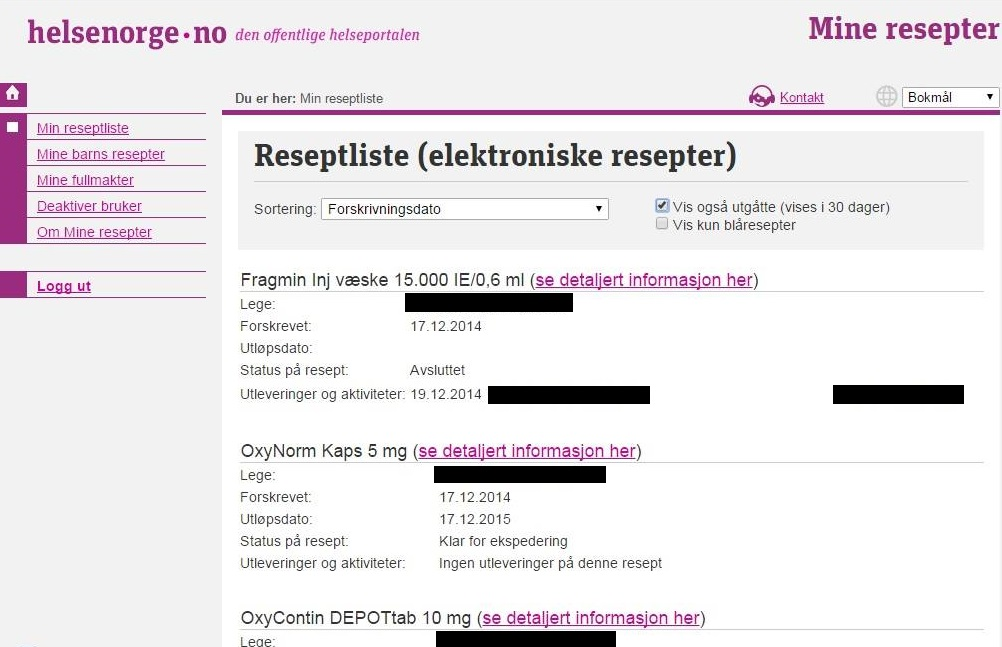
\includegraphics[width=1\textwidth]{fig/dagens/mineresepter.jpg}
  \caption{Skjermbilde som viser hvordan en reseptliste kan se ut på \url{www.minereseper.no}. Dato:19.12.2014}
\label{fig:mineResepter}
\end{figure}

\begin{figure}[H]
  \centering
    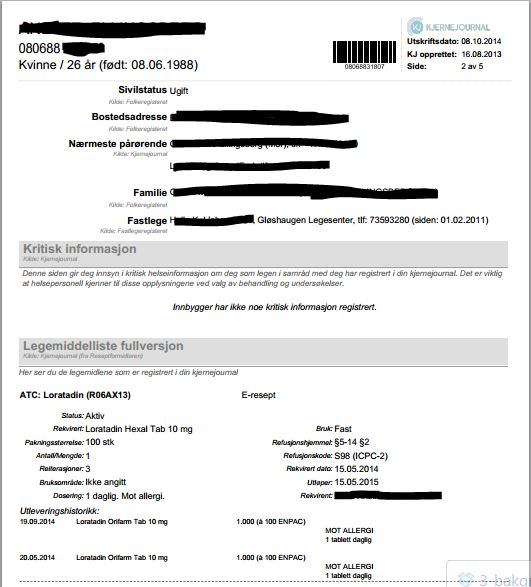
\includegraphics[width=1\textwidth]{fig/dagens/kjernejournal2.jpg}
  \caption{Skjermbilde som viser eksempel på en kjernejournal. Dato: 08.10.2014}
\label{fig:kjernejournal}
\end{figure}

\subsection{Kjernejournal}
Innbyggere i noen kommuner har tilgang til kjernejournal via helsenorge.no. Kjernejournal er et prøveprosjekt i enkelte kommuner i landet, med mål om å samle helseopplysninger på ett sted. Ved ulykke i utlandet kan det være betryggende for den utsatte å ha tilgang til egne helseopplysninger uten å være avhengig av samordning på tvers av landegrenser.

Kjernejournal er et supplement til journaler som føres hos lege eller på sykehus, og inneholder helseopplysninger som kan være viktige for helsepersonell å vite om, spesielt i akutte situasjoner. Opplysningene hentes automatisk fra offentlige register, blant annet personalia (fra Folkeregisteret), fastlege (fra Fastlegeregisteret), legemidler utlevert på resept i norske apotek (Reseptformidleren\footnote{Reseptformidleren er en nasjonal elektroniske database for behandling av reseptopplysninger}) og tidligere kontakt med spesialisthelsetjenesten (Norsk pasientregister). Se figur~\ref{fig:kjernejournal} for et eksempel på hvordan en kjernejournal ser ut.

\subsection{Felleskatalogen}
Felleskatalogen er en oversikt over legemidler som markedsføres i Norge. Informasjonen er sortert etter handelsnavn på legemidler. Bransjeforeningen for legemiddelindustrien utgir Felleskatalogen. Den er produsentavhengig, noe som kan påvirke hvilken informasjon som inkluderes og hvordan informasjonen vinkles. Felleskatalogen er tilgjengelig i bokform, på internett\footnote{Felleskatalogen på nett finner du på \url{www.felleskatalogen.no}} og som applikasjon til smarttelefon og nettbrett. Figur~\ref{fig:felleskatalogen} viser et skjermbilde fra felleskatalogen på nett. 

I felleskatalogen på internett ligger pakningsvedlegg til alle legemidler som markedsføres i Norge. 

\begin{figure}[H]
  \centering
    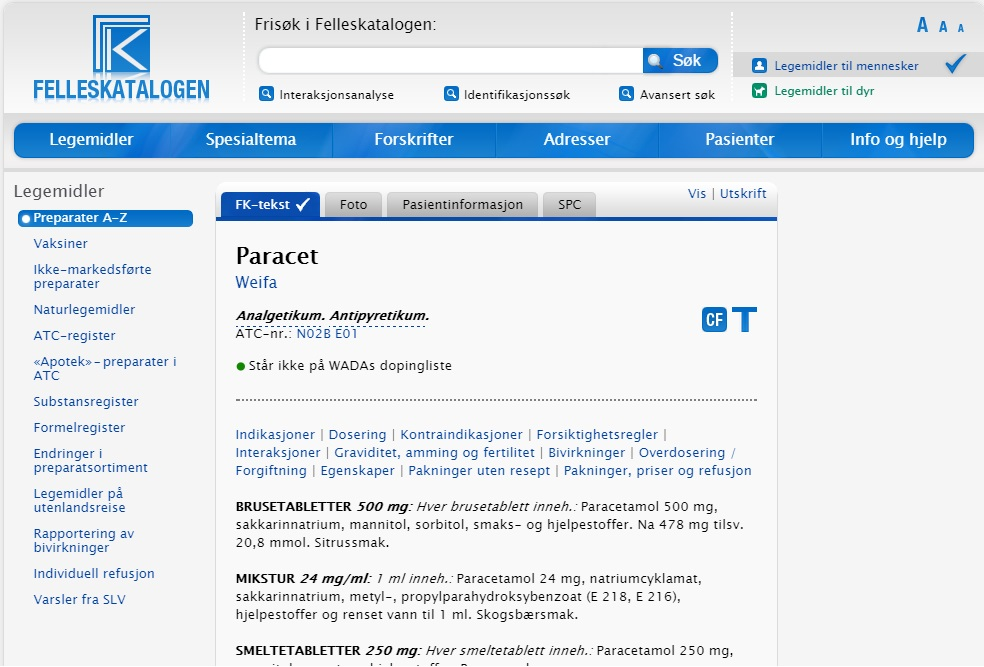
\includegraphics[width=1\textwidth]{fig/dagens/paracetFelleskatalog.jpg}
  \caption{Skjermbilde som viser informasjon om Paracet i Felleskatalogen på internett. Dato: 30.10.2014}
\label{fig:felleskatalogen}
\end{figure}


\subsection{Legemiddelhåndboken}
Legemiddelhåndboken (Norsk legemiddelhåndbok for helsepersonell) er et terapiorientert oppslagsverk for legemidler som behandlingsalternativ. Legemiddelhåndboken er en viktig kilde til leverandørnøytral informasjon om indikasjoner, bruk, virkninger og bivirkninger av legemidler. 
 
Legemiddelhåndboken er rettet mot leger. Det er derfor lagt særlig vekt på å omtale tilstander hvor legemidler har en viktig plass i behandlingen.
 
Legemiddelhåndboken er delt i fire hovedavsnitt:
\begin{itemize}
    \item en del om sykdommer
    \item en del om legemidler
    \item en generell del som omfatter ulike behandlingssituasjoner og veiledning ved legemiddelbruk
    \item en registerdel med blant annet stikkord og adresseregister
\end{itemize}

\acrshort{start}\footnote{Les mer om START her: \url{http://legemiddelhandboka.no/Generelle/311103}}, \acrshort{stopp}\footnote{Les mer om STOPP her: \url{http://legemiddelhandboka.no/Generelle/315753}} og \acrshort{norgep}\footnote{Les mer om NorGep her: \url{http://legemiddelhandboka.no/Generelle/311393}} er tatt med i legemiddelhåndboken, jf. delkapittel~\ref{subsec:legemiddelgjennomgang}.

Norsk legemiddelhåndbok er tilgjengelig på flere format: den er tilgjengelig på internett \footnote{Legemiddelhåndboken på nett finner du her: \url{www.legemiddelhandboka.no}}, den kan lastes ned lokalt til PC og den er tilgjengelig som en applikasjon til smarttelefoner. Figur~\ref{fig:legemiddelhandbok} viser et skjermbilde fra legemiddelhåndboken på nett.

\begin{figure}[H]
  \centering
    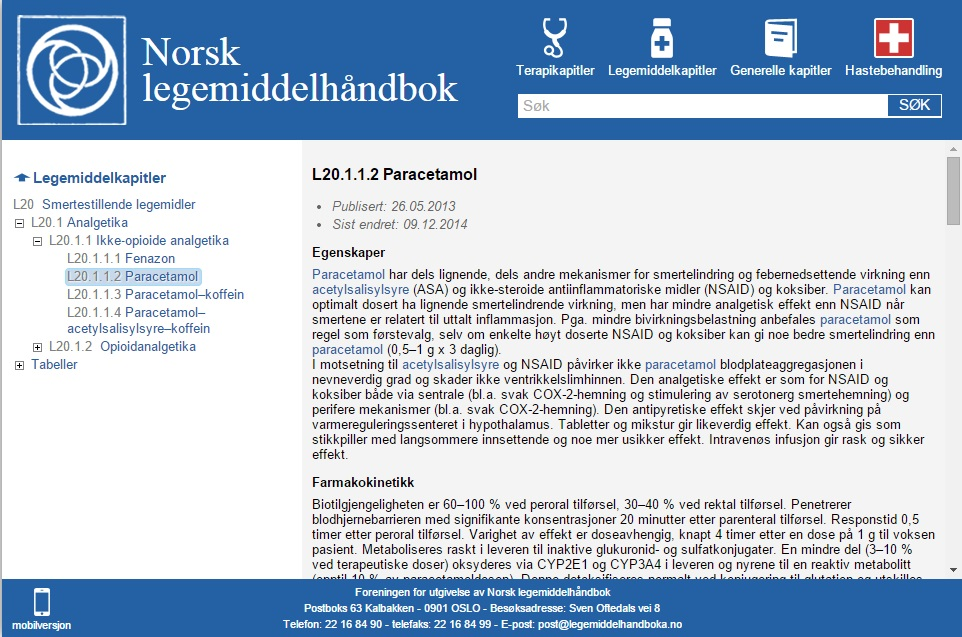
\includegraphics[width=1\textwidth]{fig/dagens/paracetLegemiddelhandbok.jpg}
  \caption{Skjermbilde som viser informasjon om Paracetamol i legemiddelhåndboken på internett. Dato: 30.10.2014}
\label{fig:legemiddelhandbok}
\end{figure}


\subsection{FEST}
\acrfull{fest} er en database utviklet av Legemiddelverket. Databasen inneholder informasjon om alle legemidler som kan kjøpes på resept i Norge. Målet med \acrshort{fest} er å fremme trygg legemiddelbruk, og gi oppdatert og samstilt informasjon til leger, apoteker og bandasjister. \acrshort{fest} presenterer data i \acrshort{xml}-format\footnote{XML: er et markeringsspråk som definerer et sett av regler for koding av dokumenter til et format som både kan leses av mennesker og maskiner.} og en er viktig del av datagrunnlaget for andre systemer, blant annet en forutsetninger for innføring av e-Resept \citep{omFEST}. 

\subsection{Interaksjoner.no}
Interaksjoner.no er et verktøy for å søke etter legemiddelinteraksjoner ved å bruke norske handelsnavn. Interaksjoner.no er basert på \acrshort{fest}, og det er Legemiddelverket som er ansvarlig for innholdet i databasen. 

Motivasjonen for å utvikle verktøyet er at manuelle oppslag på mulige interaksjoner for hvert enkelt legemiddel er tidkrevende, og at andre systemer for å sjekke interaksjoner ikke gjenkjenner norske handelsnavn \citep{OmInteraksjonerdotno}. 

Figur~\ref{fig:int} viser et skjermbilde fra interaksjoner.no med resultater ved søk på Albyl-E. I listen over interaksjoner er det brukt \acrshort{atc}-koder istedenfor norske handelsnavn på legemidler. Dette kan gjøre det vanskelig for pasienter å forstå hvilke legemidler som er delaktig i interaksjonene.

\begin{figure}[H]
  \centering
    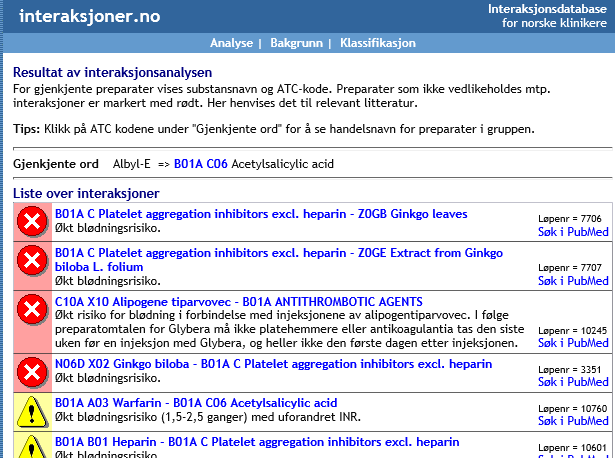
\includegraphics[width=1\textwidth]{fig/dagens/interaksjoner.png}
  \caption{Skjermbilde fra \url{www.interaksjoner.no} som viser resultatet av søk på Albyl-E. Dato: 09.11.2014}
\label{fig:int}
\end{figure}

\subsection{RELIS}
\acrshort{relis} (\acrlong{relis}) er en offentlig finansiert informasjonstjeneste som skal gi produsentuavhengig legemiddelinformasjon til helsepersonell. Hensikten er at \acrshort{relis} skal bidra til forsvarlig, rasjonell og riktig bruk av legemidler.
 
Ved universitetsykehus i alle de fire helseregionene er det etablert \acrshort{relis}-sentre. Alle sentrene er knyttet til de klinisk farmakologiske fagmiljøene ved universitetssykehusene, og har et bredt samarbeid med helsepersonell i regionene. På \url{www.relis.no/database} har \acrshort{relis} en spørsmål-svar tjeneste, se figur~\ref{fig:int}. Tjenesten er beregnet på helsepersonell, og er ment å være til hjelp med legemiddelspørsmål.

\begin{figure}[H]
  \centering
    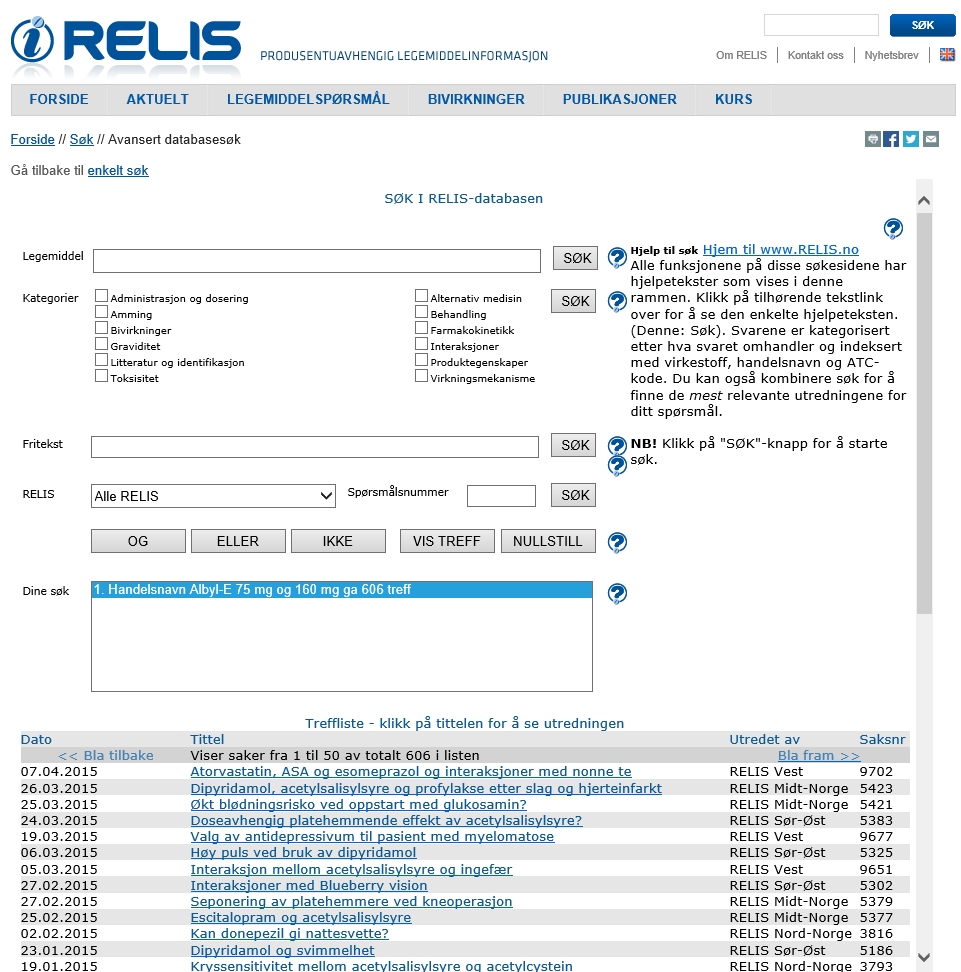
\includegraphics[width=1\textwidth]{fig/dagens/relis.png}
  \caption{Skjermbilde som viser \url{www.relis.no/database} ved søk på Albyl-E.  Dato: 15.02.2015}
\label{fig:relis}
\end{figure}

\acrshort{relis} har ansvaret for bivirkningsovervåkningen på oppdrag fra Statens Legemiddelverk. De mottar bivirkningsmeldinger, vurderer hendelsesforløp og årsakssammenheng og kommentarer i skriftlig tilbakemelding til melder. Bivirkningsrapportene blir registrert i en nasjonal bivirkningsdatabase.


\section{Pasientkontrollerte systemer}
Her presenteres pasientkontrollerte systemer som er utviklet av store internasjonale selskaper, men som er lite tatt i bruk i Norge. 

\subsection{Google Health}
Google Health var en personlig helsejournal laget av Google. Systemet fungerte ved at brukere la inn helseinformasjon manuelt eller ved dataoverføring fra helsetjenesten. Når informasjon var lagt inn i systemet kunne Google Health vise brukeren en personlig journal og vise mulige interaksjoner mellom legemidler. I 2011 annonserte Google at Google Health skulle legges ned. Figur~\ref{fig:googleHealth} viser et skjermbilde av hvordan Google health så ut da det eksisterte. 

\subsection{Microsoft HealthVault}
Microsoft HealthVault er en skybasert plattform som skal lagre og vedlikeholde helse- og fitnessinformasjon. Systemet fungerer som en egenopprettet journal hvor brukeren styrer innhold og tilgang. Opplysningene kan legges inn manuelt av brukerne, eller automatisk fra utstyr som kan kobles opp mot HealthVault. Dette kan være opplysninger om legemidler, vaksinasjoner, vekt osv. 

Figur~\ref{fig:HealthVault} viser et skjermbilde av HealthVault-profilen til Kåre. Det er lagt inn informasjon om Kåre sine legemidler og lidelser som fritekst. HealthVault er ikke i stand til å gjøre noe resonnering basert på informasjonen som er lagt inn, og Kåre kan ikke få informasjon om mulige interaksjoner eller bivirkninger. 


\subsection{Dossia}
I 2006 ble Dossia grunnlagt som et samarbeidsprosjekt mellom flere arbeidsgivere. Målet var å gi sine ansatte en helsejournal. Dossia er en personlig helsejournaltjeneste. Den gjør det mulig for pasienter å samle kopier av sine egne helsedata fra ulike steder, for å lage en personlig og elektroniske helsejournal.

\subsection{Indivo}
Indivo er en helsejournalplattform laget av \acrfull{chip}. Den fokuserer på å gi brukere kontroll over egen helsejournal. Det er en plattform som muliggjør utvikling av personlige helseapplikasjoner hvor pasienter kan se og legge inn merknader til informasjonen. Indivio har blitt brukt i Microsoft sitt prosjekt HealthVault, har inspirerte arkitekturen til Google Health og har blitt brukt i Dossias helsejournal.

\begin{figure}[H]
  \centering
    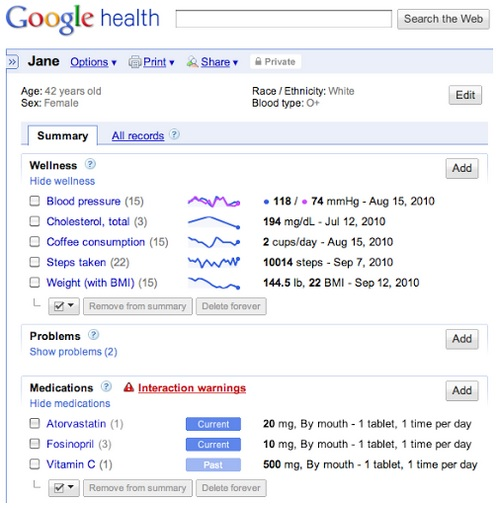
\includegraphics[width=1\textwidth]{fig/dagens/GoogleHealth.jpg}
  \caption{Skjermbilde som viser hvordan GoogleHealth så ut. Hentet fra: \url{http://googleblog.blogspot.no/2010/09/google-health-update.html}}
\label{fig:googleHealth}
\end{figure}

\begin{figure}[H]
  \centering
    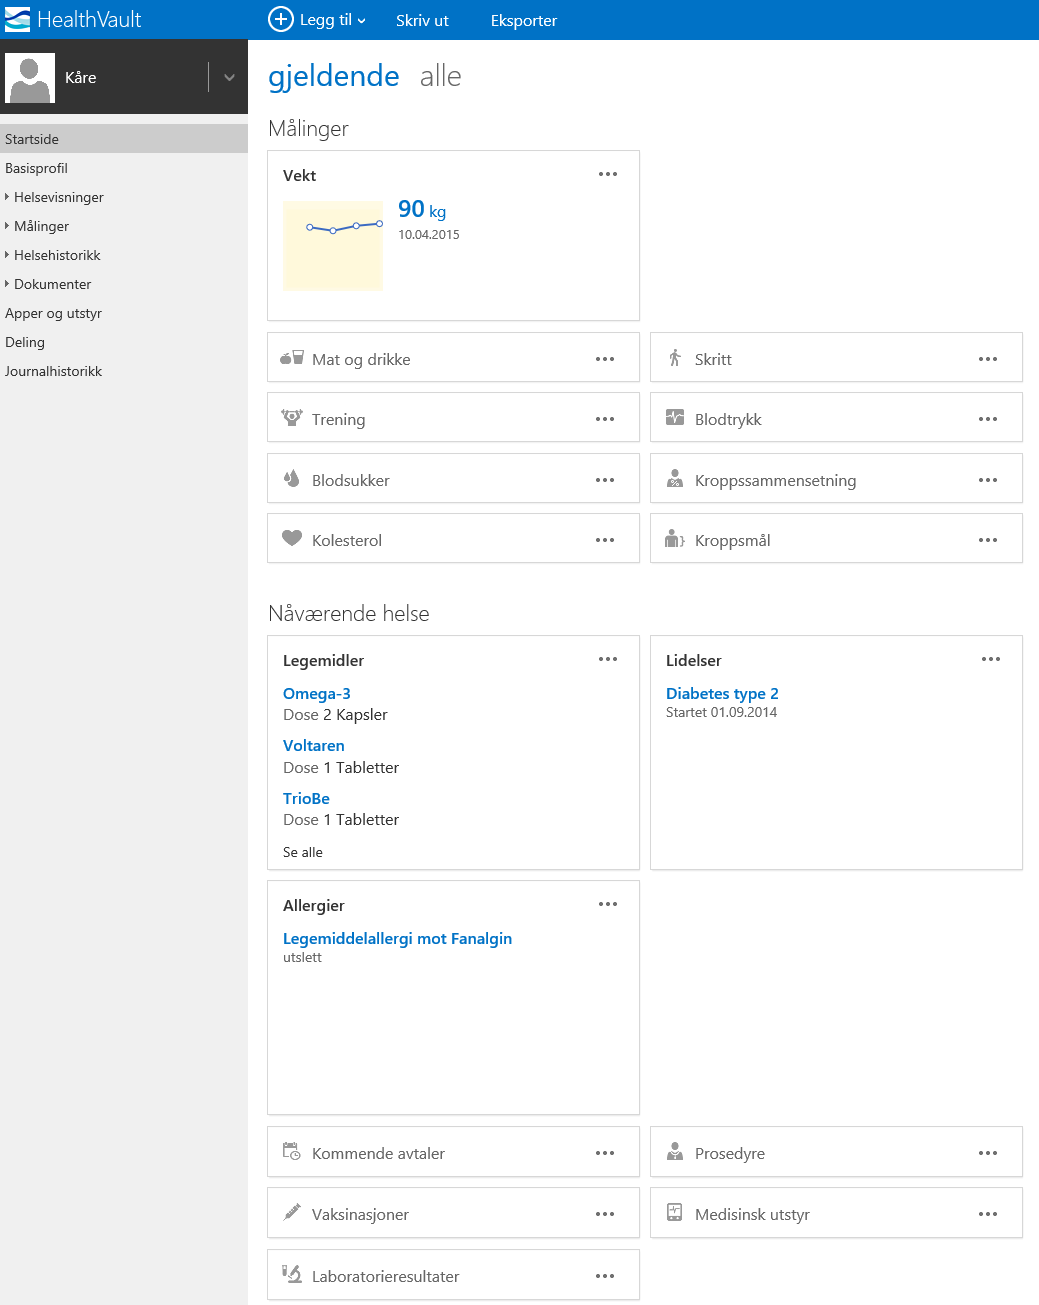
\includegraphics[width=1\textwidth]{fig/dagens/HealthVault.png}
  \caption{Skjermbilde fra HealthVault for Kåre 77 år. Dato 10.04.2015}
\label{fig:HealthVault}
\end{figure}


\section{Personvern} \label{sec:sikkerhet}
Økt bruk av elektronisk behandling av informasjon og personopplysninger skaper mange muligheter, men det medfører også utfordringer for personvern. Elektronisk behandling av opplysninger om pasienter medfører at opplysningene lett kan bli tilgjengelig både internt i helsevesenet og eksternt for pasienter og pårørende. Det er viktig å passe på at uvedkommende ikke får tilgang til opplysninger som er lagret elektronisk. I det følgende blir viktige lover og regler som skal sikte at personvernet er ivaretatt av legemiddelinformasjonskilder presentert kort.


\subsection{Lov om medisinsk utstyr}
Det norske lovverket er i samsvar med \acrshort{eu}s bestemmelser vedrørende medisinsk utstyr (medical devices), jf. direktiv 2007/47/EC. Lov om medisinsk utstyr regulerer “produksjon, markedsføring, omsetning og bruk av medisinsk utstyr”, jf. lov om medisinsk utstyr § 1. Formålet med loven er å forhindre skader og å sikre at medisinsk utstyr blir brukt på forsvarlig måte, jf. lov om medisinsk utstyr § 2.

Det er gitt detaljerte regler om merking av medisinsk utstyr, og om hvordan produsenter skal gå frem for å sikre og dokumentere at utstyret fyller de tekniske krav som er satt. Utstyr som er fremstilt i samsvar med regelverket, skal \acrshort{ce}-merkes\footnote{CE-merke er et godkjenningsmerke innenfor EØS-området}, jf. lov om medisinsk utstyr § 5 og forskrift om medisinsk utstyr § 2-4.

For å falle under lovens definisjon av medisinsk utstyr må det være “ment å skulle brukes på mennesker”, jf. lov om medisinsk utstyr § 3 første ledd. Det er noe uklart hvorvidt kilder til personlige legemiddelinformasjon faller under ordlyden av dette. Lov om medisinsk utstyr § 3 fjerde ledd, angir at det i tvilstilfeller er departementet som avgjør om noe er å regne som medisinsk utstyr.
 
Generelt sett skal sosial- og helsedirektoratet føre tilsyn med at regelverket om medisinsk utstyr overholdes. Direktoratet for samfunnssikkerhet og beredskap har også en tilsynsrolle når det gjelder elektronisk medisinutstyr.

\subsection{Personopplysningsloven og helseregisterloven}
I Norge stiller Personvern- og helselovgivningen krav til informasjonssikkerhet\footnote{Informasjonssikkerhet: samlebetegnelse for krav til påliteligheten og sikkerheten som knyttes til informasjon.}. Aktuelle tilsynsmyndigheter (Datatilsynet og Helsetilsynet) har ansvar for å kontrollere etterlevelse av gjeldende regelverk.
 
Personopplysningsloven gir grunnleggende regler innen personvern og informasjonssikkerhet. I Helseregisterloven finnes regler om hvordan virksomheter skal behandle pasienters helseopplysninger. Kravene i helseregisterloven er harmonisert med de generelle kravene som gjelder ved behandling av personopplysninger etter personopplysningsloven. Dette er fordi begge lovene bygger på EUs personverndirektiv (95/46/EF), og fordi det ikke er ønskelig med utvikling av forskjellige sikkerhetsnivåer i forskjellige samfunnssektorer \citep{kommentarutgaveHelseregisterloven}.
 
Formålet med helseregisterloven er å bidra til at helseopplysninger kan samles inn og brukes til helsefremmende formål, uten å krenke personvernet, jf. helseregisterloven § 1. Opplysninger  registrert om en pasient i et digitalt system er etter loven regnet som «helseopplysninger», jf. helseregisterloven § 2 bokstav a. Personlige systemer for legemiddelinformasjon må derfor følge bestemmelsene i helseregisterloven om behandlingen av helseopplysninger.

\subsection{Normen}
Sosial- og helsedirektoratets tok initiativ til at helsesektoren skulle utarbeide sin egen norm for informasjonssikkerhet. Dette resulterte i norm for informasjonssikkerhet i helse-, omsorgs- og sosialsektoren (Normen). Det er en samling retningslinjer og krav som skal bidra til “tilfredsstillende” informasjonssikkerhet hos virksomheter i sektoren. Normen gjelder for alle virksomheter som ved avtale har forpliktet seg til å følge den \citep{OmNormen}.

\chapter{Eksperimentdesign} \label{chap:eksperimentdesign}
Frem til nå har motivasjon, bakgrunn og dagens situasjon for oppgaven blitt presentert. Nå er det på tide å se på denne oppgavens bidrag til forskningen. I dette kapittelet presenteres eksperimentdesignet for oppgaven i form av en overordnet forskningsplan.

\section{Valg av forskningsmetode}
Forskningsmetoder deles inn i to grupper: Kvalitativ og kvantitativ. Ved bruk av kvalitativ metode går man i dybden på et tema ved hjelp av samtaler, intervju eller observasjon. Kvantitativ metode fokuserer på å få en bredere forståelse av et tema ved å samle data fra mange deltakere \citep{Halvorsen1993}.

Forskningsspørsmålet legger føringer på valg av metode i oppgaven:
\thesisRQ

For å kunne ta stilling til forskningsspørsmålet planlegger vi å bruke en kvalitativ metode for å sammenligne en digital prototype og pakningsvedlegg. Den digitale prototypen kalles \textit{Mine Medisiner}. Eksperimentet skal undersøke de to systemenes måte å presentere legemiddelinformasjon på. Eksperimentet består av flere kasus. I hver kasus utfører én person(deltaker) et sett med forhåndsdefinerte oppgaver ved hjelp av enten pakningsvedlegg eller prototypen. Vi skal observere deltakerne mens de utfører oppgavene for å få et inntrykk av hvordan de interagerer med det aktuelle systemet. 

Ved gjennomføring av eksperimenter for å sammenligne to systemer, bør systemene være like ``ferdige'' \citep{toftoy2011praktisk}. Det er som regel ikke gunstig å sammenligne en prototype med et ferdig system. For å få gode resultater må vi derfor påse at begge systemene blir like ferdige for de oppgavene som skal utføres i eksperimentet. Eksperimentet skal inneholde oppgaver som er mulig å løse tilfredsstillende ved bruk av både den digitale prototypen og pakningsvedlegg.

\section{Arbeidsprosessen}
Vi har følgende forskningsplan:
\begin{enumerate}
\item Gjennomføre litteraturstudium for å undersøke ulike tema innenfor problemområde (Kapittel~\ref{chap:lit}).
\item Utvikle en digital prototype: Mine Medisiner (Kapittel~\ref{chap:utvikleprototype}).
\item Utføre eksperiment på pakningsvedlegg og Mine Medisiner (Kapittel~\ref{chap:gjennomforing}).
\item Analysere resultat av eksperimentet (Kapittel~\ref{chap:resultat}).
\end{enumerate}

Arbeidet vil starte med et litteraturstudium for å undersøke problemområdet og hva som er gjort tidligere. 

Vi skal sammenligne pakningsvedlegg og Mine Medisiner sine måter å presentere informasjon. For å kunne gjøre dette må Mine Medisiner utvikles. På grunn av begrenset tid anser vi det ikke som realistisk å få utviklet en ferdig versjon av Mine Medsiner. Vi skal derfor utvikle en digital prototype vil bli hardkodet til å bare fungere for et fåtall fiktive pasienter. 

For å gjøre sammenligning av Mine Medisiner og Pakningsvedlegg vil vi utføre forsøk på begge systemene. Resultatet av disse forsøkene vil til slutt bli analysert for å undersøke hvilke påstander de underbygger.

\section{Rekruttere deltakere}
For å få best mulig resultater ønsker vi at deltakerne i størst mulig grad skal kunne relatere til oppgavene og legemidlene som blir brukt i eksperimentet. Eksperimentet kan imidlertid ikke basere seg på deltakernes virkelige legemiddelsituasjon fordi denne informasjonen er sensitiv. Planen er å rekruttere \acrshort{tia}\footnote{TIA: Hjerneslag hvor symptomene trekker seg tilbake i løpet av 24 timer}-pasienter til eksperimentet, og at oppgavene som skal gjennomføres skal baseres på en fiktiv \acrshort{tia}-pasient. Prototypen av Mine Medisiner må derfor tilpasses denne fiktive \acrshort{tia}-pasienten. 

\acrshort{tia}-pasienter kan være vanskelig å rekruttere fordi det er en snever gruppe vi har liten kjennskap til. Planen er å gjøre rekrutteringen gjennom kontakter på St. Olav.


\section{Analyseplan}
Underveis i arbeidet med masteroppgaven vil vi skrive en felles forskerlogg i et delt dokument på internett. Denne forskerloggen vil inneholde alt av tanker og idéer vi har underveis. 

Vi vil gjennomføre mange møter underveis i arbeidsprosessen. Før alle møtene vil vi utarbeide møteplaner i delte dokumenter på internett. Under møtene fylles dette dokumentet inn med referat av det som blir sagt og gjort.

For hver deltaker vil vi lage et delt dokument som inneholder viktige punkter for hva vi skal notere underveis i gjennomføringen. På den måten går det raskere å ta notater. Etter hver kasus renskrives notatene for å sikre at de er forståelige til senere bruk. Det vil også tas vare på eventuelle skjema som deltakerene fyller ut. Det vil føres på et identifiserende tall på alt materiale fra hver deltaker, for å kunne skille kasusene fra hverandre. 

Datamaterialet fra kvalitative analyser er gjerne omfattende og ustrukturert. Notater fra kasus, forskerlogg og møtereferater vil for oss utgjøre det \citep{patton2002qualitative} kaller den ufordøyde, komplekse virkelighet. For å bearbeide dette ustrukturerte materiale vil vi benytte oss av en prosess kalt \textit{åpen koding}. Ved åpen koding løsriver man seg fra forskningsspørsmålet og skriver ned alt man ser. I denne prosessen gis navn til ulike deler av datamaterialet. Disse navnene kalles koder. For eksempel kan man skrive koder i margen som forklarer hva hvert avsnitt i en tekst inneholder \citep{nilssen2012analyse}. 

Etter kodeprosessen vil vi sitte igjen med veldig mange koder. I det neste steget vil vi klassifisere kodene, ved å se på sammenhengen mellom dem og hvilke mønstre de danner. Klassifiseringene skal beskrive essensen i datamaterialet og danne basis for å skrive om resultatet av eksperimentet(kapittel~\ref{chap:resultat}). Resultatene skal brukes til å underbygge påstander (kapittel~\ref{chap:analyse}). For å vurdere hvor bastante påstander vi kan komme med vil vi se på signifikansen av resultatene de underbygges av.


\section{Oppnå gode resultater} 
Feilkilder vil alltid påvirke resultatene i et forskningsprosjekt. Feil kan oppstå i alle faser av arbeidet. Ved å være klar over potensielle feilkilder er det mulig å ta hensyn til dem, og minimere påvirkningen av feilene.

Validitet\footnote{Les mer om validitet her: \url{https://sml.snl.no/validitet}} betyr gyldighet, og måler i hvilken grad det kan trekkes gyldige slutninger ut i fra en undersøkelse. For eksempel måler validiteten av eksperimentet vårt i hvor stor grad eksperimentet gir oss svar på forskningsspørsmålet vår.

Indre validitet handler om hvorvidt resultatene er gyldige for utvalget og eksperimentet som er gjennomført. Indre validitet kan være vanskelig fordi faktorer man ikke har kontroll over kan påvirke resultatene. Den indre validiteten av resultatene kan bli svekket ved at deltakerne påvirkes av de som utfører eksperimentet. For å øke den indre validiteten av eksperimentet skal vi ha en prøvegjennomføring for å finne svakheter i oppsettet, og gjøre forbedringer før den ordentlige gjennomføringen. 

Ytre validitet handler om hvorvidt et resultat kan overføres til andre enn de som deltok på undersøkelsen. Dersom utvalget er veldig skjevt, og ikke gjenspeiler befolkingen, kan det føre til lav ytre validitet. For å sørge for at den ytre validiteten ikke blir for lav skal vi prøve å rekrutere et representativt utvalg av \acrshort{tia}-pasienter. Det at vi planlegger å bare ha deltakere som er \acrshort{tia}-pasienter gjør at eksperimentet ikke nødvendigvis blir overførbart til målgruppen vår for øvrig. 

Ytre validitet kan være en utfordring når kunstige situasjoner skapes i forsøkssammenheng. For å motvirke dette skal vi gjennomføre kasusene uten å forstyrre deltakerne unødig underveis.

Hawthorne-effekt er når noens adferden endres fordi de blir studert\footnote{Les mer om Hawthorne-effekten her: \url{https://snl.no/Hawthorneeffekten}}. I forskning er det et mål å studere noe slik det er. Dersom forskningen i seg selv påvirker resultatene vil de være ugyldige. Vi vil forsøke å ikke kommentere ting underveis i gjennomføringen av forsøkene slik at deltakerne ikke blir påminnet at de blir observert mer enn nødvendig. Ting som skal diskuteres vil derfor bli tatt opp helt til slutt. 

Reliabilitet\footnote{Les mer om reliabilitet her: \url{https://sml.snl.no/reliabilitet}} betyr pålitelighet, og måler i hvilken grad man får samme resultat dersom en undersøkelse gjentas. Vi planlegger å bare ha 10-15 deltakere. Et så lavt antall kan gi litt lav pålitelighet. For å kunne få pålitelige resultater tross det lave antallet deltakere skal vi gjennomføre eksperimentet på en liten deltakergruppe (\acrshort{tia}-pasienter). Ved å ha en liten og veldefinert gruppe med deltakere tror vi det er større sannsynlighet for at deltakerne kan bli representative for gruppen og at det derfor vil gi samme resultatet å gjøre eksperimentet på nytt.



\chapter{Litteraturstudier}\label{chap:lit}

I dette kapittelet blir resultatet av litteraturstudier vi har utført på ulike tema innenfor problemområdet presentert.

Et litteraturstudium er en systematisk gjennomgang av litteraturen rundt et valgt problemområde. I et litteraturstudium bør det foretas en kritisk gjennomgang av kilder, og kildene bør diskuteres. En kritisk gjennomgang av søkeresultatene er viktig fordi et søk kan gi for mange (for vide søkeord) eller for få treff (for snevre søkeord). Antall siteringer en artikkel har kan bli brukt som en kvalitetsidentifikator på resultatene, og for å få en indikasjon på aktualiteten av søkeresultatene.  

Med utgangspunkt i oppgavens problemområde definerte vi ulike begreper og nøkkelord vi antok var dekkende for det vi ønsket å undersøke. Vi kategoriserte begrepene og nøkkelordene for å finne resultater basert på kombinasjoner av ordene. I tillegg til å søke etter artikler gjorde vi såkalt “snowballing”, som innebar at vi fulgte siteringer i artiklene vi fant for å finne flere relevante artikler.

Databasene vi brukte for litteraturstudiene var: PubMed, Google Scholar, tidsskriftet.no. BIBSYS Ask, Cochrane Library, UpToDate og IEEE Xplore Digital Library.


\section{Legemiddelgjennomgang} \label{sec:littLegemiddelgjennomgang}
Målet med Mine Medisiner er å gi pasienter bedre oversikt over egen legemiddelsituasjon. Dette kan føre til at pasienten kan bidra mer ved legemiddelgjennomgangen, jf. delkapittel~\ref{subsec:legemiddelgjennomgang}. Vi gjorde et litteraturstudium for å undersøke hvilke verktøy som i dag finnes for legemiddelgjennomganger, og hvilke forskning som er gjort på hva som kan gjøre legemiddelgjennomganger lettere.  

Ved å utføre legemiddelgjennomgang kan pasienter få bedre effekt av legemiddelbehandling og oppleve færre bivirkninger. Pasienten kan også oppleve å få et mer hverdagstilpasset legemiddelregime etter en legemiddelgjennomgang. Dette gir bedret livskvalitet, og kan føre til bedre etterlevelse \citep{stmeld1820042005, legemiddelgjennomgangVeileder, MedicationReview}.

Et samfunn hvor pasienten har bedre livskvalitet og bedret etterlevelse vil redusere behovet for helse-, pleie- og omsorgstjenester. Dette gir en reduksjon i samfunnets helsekostnader. En videre reduksjon i helsekostnadene kan også oppstå fordi legemiddelgjennogmanger ofte fører til en reduksjon i antall legemidler i legemiddellisten til pasienten \citep{HealthEconomic}.

Legemiddelgjennomganger kan gi fordeler både for pasienten og samfunnet. Legemiddelgjennomgang er derfor blitt viktig i helsetjenesten. I dag jobbes det for at pasientinvolvering skal bli en større del av helsetjenesten. Allikevel finnes det ikke tjenester for pasientsentrerte legemiddelgjennomganger per dags dato \citep{innoMedForprojekt}. 

Det jobbes med å finne måter å gjøre legemiddelgjennomgang lettere. Legemiddelverket lanserte i 2014 en sjekkliste\footnote{Sjekkliste: liste over ting som skal sjekkes. En ting på listen kan sjekkes av når noe er blitt gjennomført, kjøpt eller lignende} for legemiddelgjennomgang. Legemiddelverkets sjekkliste er beregnet for studenter, leger og helsepersonell som er ukjent med legemiddelgjennomgang. Håpet er at sjekklisten skal føre til en enklere og raskere innføring til legemiddelgjennomgangprosessen, men forskning på om dette er tilfellet er ikke publisert enda. 

Sjekklisten for legemiddelgjennomgang er utviklet for å erstatte kliniske retningslinjer\footnote{Retningslinjer: systematiske utviklede råd og anbefalinger utarbeidet for å støtte helsepersonell og pasienter i konkrete helserelaterte situasjoner} og veiledere. Retningslinjer har vist seg   å være vanskelige å følge og lite brukt i praksis \citep{utposten, 19878542}. Retningslinjer tar ikke for seg sammensatte plager og problemer som kan oppstå ved å ha flere diagnoser. Bruk av sjekklister har vist seg å være lettere å benytte under pasientbehandlinger enn retningslinjer \citep{haugen2014effect, legemiddelgjennomgangTiltak}.

Problemet med bruk av sjekklister er at de ofte blir for generelle til å kunne tilpasses den enkelte pasient. Det er derfor viktig at leger involverer pasienten når det gjelder planlegging og endring av legemiddellisten. Legemiddelverkets sjekkliste kan føre til at det blir for stort fokus på det farmakologiske med legemiddellisten i stedet for den enkelte pasientens behov \citep{legemiddelgjennomgangTiltak}.

InnoMed\footnote{InnoMed er et nasjonalt kompetansenettverk for behovsdrevet innovasjon i helsesektoren.} har et prosjekt får å utvikle et verktøy som skal gjøre legemiddelgjennomgang lettere. Hensikten med prosjektet er å benytte seg av kommunikasjonsteknologi under legemiddelgjennomganger for å gjøre det lettere og mer kostnadseffektiv å oppnå dialog mellom tverrfaglig helsepersonell. Prosjektet fokuserer ikke på å involverer pasienten i legemiddelgjennomgangen \citep{innoMedForprojekt}.  

Slik situasjonen er i dag er det vanskelig for leger og annet helsepersonell å få oversikt over en pasients helsesituasjon. Legemiddelverkets sjekkliste og prosjektet til InnoMed er skritt i riktig retning, men de er lite tilpasset den enkelte pasient \citep{legemiddelgjennomgangTiltak}. 


\section{Medisinsk informasjonsvisualisering}
Målet for masteroppgaven var å undersøke ulike måter å presentere legemiddelinformasjon for pasienter. Et litteraturstudium på medisinsk informasjonsvisualisering ble utført for å undersøke hva som allerede er avdekket gjennom forskning på dette området. Felles for forskningen som er gjort på visualisering er at målgruppen er helsepersonell og forskere.

\subsection{GraphSaw} 
GraphSaw er et beslutningsstøttesystem\footnote{Beslutningsstøttesystem: datasystemer som skal hjelpe klinikere med å ta beslutninger i pasientbehandling.} som muliggjør utforskning av interaksjoner og bivirkninger ved at de visualiseres i en graf. Grafen danner et nettverk av legemidler og sykdommer på forskjellige farmasøytiske og molekylære nivåer. Skjembildet i figur~\ref{fig:graphsaw} viser hvordan nettverket gir informasjon om hvordan legemidlene fungerer sammen. Målet med GraphSaw er å redusere risikoen for feilmedisinering \citep{shoshi2015graphsaw}.  

Dataene GraphSaw baserer seg på er hentet fra ulike offentlig tilgjengelige databaser. GraphSaw viser hvor komplekst datagrunnlaget for legemiddelinformasjonssystemer er ved at flere kilder måtte benyttes for å danne et pålitelig system, da ingen av de eksisterende kildene inneholdt fullstendig informasjon. 

Målgruppen til systemet er helserpersonell og forskere, men visualiseringsprinsippene er antagelig overførbare til pasiententrettede systemer. Systemet viser at grafer kan brukes til å representere nettverk av legemiddelrelatert informasjon.

\begin{figure}[H]
  \centering
    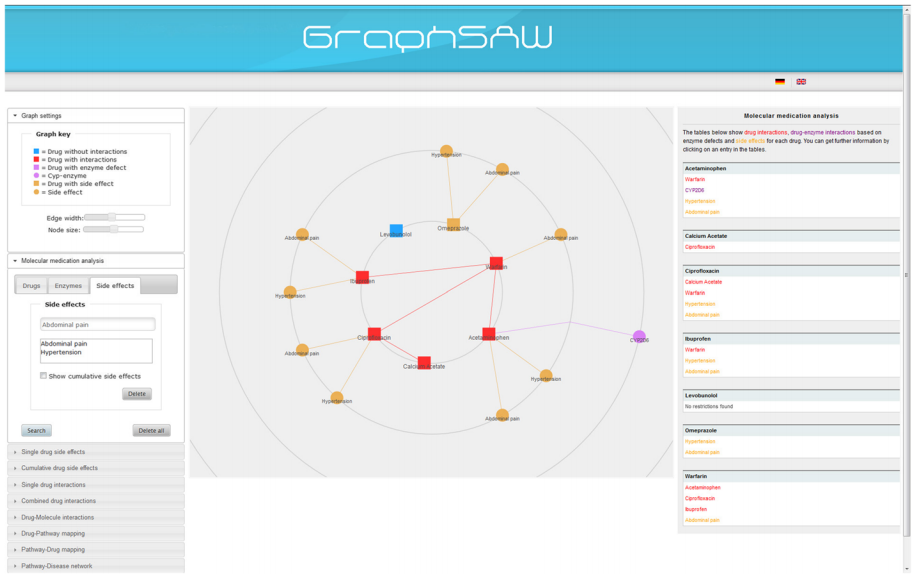
\includegraphics[width=1\textwidth]{fig/litteratursok/graphsaw.PNG}
  \caption{Nettverk av legemiddelinformasjon i Graphsaw. Nettverket viser interaksjoner mellom legemidler (røde noder), interaksjoner mellom legemiddler og enzymer (lilla noder), legemiddelbivirkninger (gule noder) og legemidler uten potensielle risikoer (blåe noder). Til høyre i figuren vises informasjon om nodene og kantene i nettverket \citep{shoshi2015graphsaw}.}
\label{fig:graphsaw}
\end{figure}

\subsection{Elektroniske pasientjournaler}
\acrfull{epj} er en elektronisk samling av registrerte opplysninger om en pasient i forbindelse med helsehjelp. \acrfull{epj} kan brukes for å ta avgjørelser om enkeltpasienter og for å få kunnskap om befolkningen generelt. Løsningene er rettet mot helsepersonell. Per i dag er bruksmønsteret ofte “Skrives én gang, leses aldri” \citep{powsner1994graphical}.  

\acrshort{epj}-systemene som brukes av det norske helsevesenet i dag representerer historiske data for pasienter som fritekst. For å gjøre det enklere å utforske informasjonen og gjøre spørringer i \acrshort{epj} bør innholdet visualiseres og gjøres interaktivt \citep{spense2007information}. Interaksjon kan gi brukeren mulighet til å velge hvordan, og hvilke, data som presenteres. I de neste avsnittene gis eksempler som illustrerer hvordan \acrshort{epj} kan gjøres interaktivt. 

Historiske data kan visualiseres som hendelsesforløp bestående av punkter eller linjesegmenter på en tidslinje. Figur ~\ref{fig:lifeline_timeline} viser hvordan LifeLines\footnote{LifeLines: System for visualisering av personlige legemiddelhistorier utviklet sent på 90-tallet} bruker tidslinjer. LifeLines bruker en visualiseringsteknikk som skiller kategorier av hendelser på separate tidslinjer, og bruker farger for å skille hendelsestypene. 

\begin{figure}[H]
  \centering
    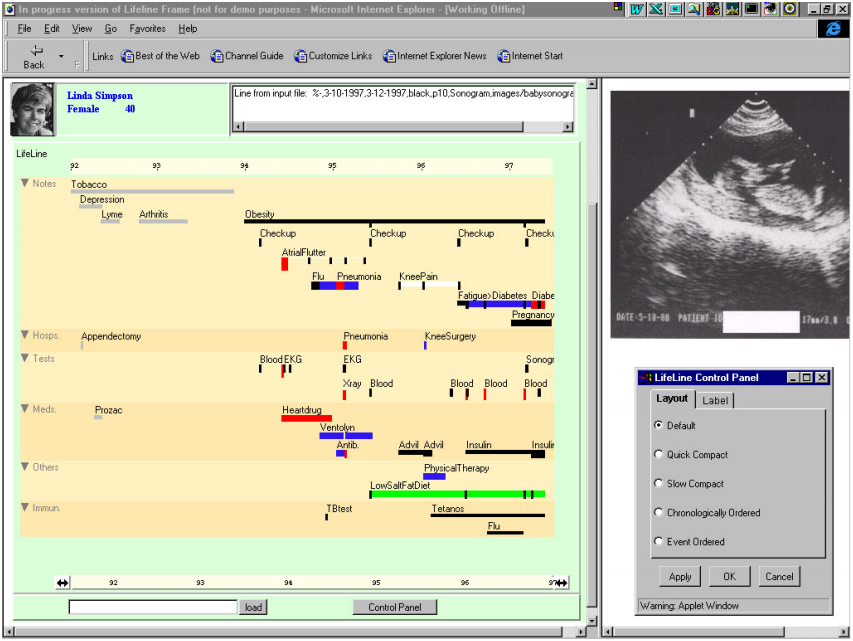
\includegraphics[width=1\textwidth]{fig/litteratursok/lifeline_timeline.PNG}
  \caption{Skjermbilde av bruk av tidslinjer i Lifelines \citep{rind2011interactive}. }
\label{fig:lifeline_timeline}
\end{figure}

LifeLines visualiserte hendelsesforløp for én pasient. Lifelines2 gjør det mulig å se fellestrekk mellom hendelsesforløpene til flere pasienter. Dette gjøres ved å sentrere forløpene rundt en felles hendelse for å få oversikt over hvordan de ulike forløpene har utartet seg før og etter hendelsen det senteres på. Figur ~\ref{fig:lifelines2} viser et skjermbilde fra Lifelifes2 hvor en hendelse representert av gule trekanter er sentrert i bildet. 

\begin{figure}[H]
  \centering
    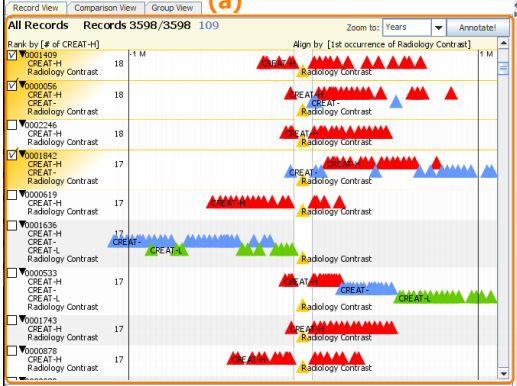
\includegraphics[width=1\textwidth]{fig/litteratursok/lifelines2.PNG}
  \caption{Justering av hendelser i tid mellom pasientforløp i Lifelines2 \citep{rind2011interactive}.}
\label{fig:lifelines2}
\end{figure}

Midgaard\footnote{Midgaard: System for visualisering av behandling på intensivavdelinger} gjør det mulig å endre nivået av detaljer på en tidslinje ved å zoome, se eksempler i figur~\ref{fig:midgaard}. Zoom gir mulighet for personlig tilpasning ved at brukeren selv kan velge detaljerningsnivået på informajsonen som vises \citep{rind2011interactive}. 

\begin{figure}[H]
  \centering
    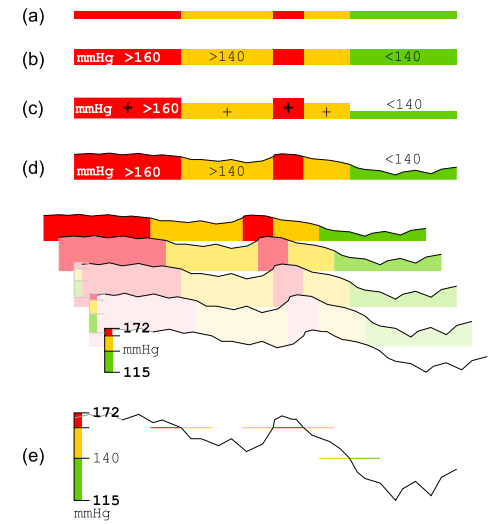
\includegraphics[width=0.6\textwidth]{fig/litteratursok/midgaard.PNG}
  \caption{Viser gradvis økning i detaljnivå ved bruk av zoom i Midgaard \citep{rind2011interactive}}
\label{fig:midgaard}
\end{figure}

Et alternativ til å vise hendelsesforløp som linjer er å bruke ikoner som består av grafiske elementer. Denne måten å visualisere pasientinformasjon på er gjort i et system kalt VIE-VISU\footnote{VIE-VISU: System som visualiserer data fra helseinformasjonssystemer.} som ble tatt i bruk på en intensivavdeling for nyfødte. Hvert ikon representerer helsetilstanden på et bestemt tidspunkt. En serie med 24 ikoner viser utviklingen av pasientens helsetilstand det siste døgnet, som vist i figur~\ref{fig:mange_glyphs}. 

Ikonene består av grafiske elementer som representerer ulike målinger for sirkulasjon, pust og veskebalanse. Størrelsen og fargen på de grafiske elementene brukes til å illustrere målingenes verdi, som vist i figur~\ref{fig:mange_glyphs}. For eksempel er pasientens registrerte puls representert ved bredden på den røde trekanten i hvert ikon.


\begin{figure}[H]
  \centering
    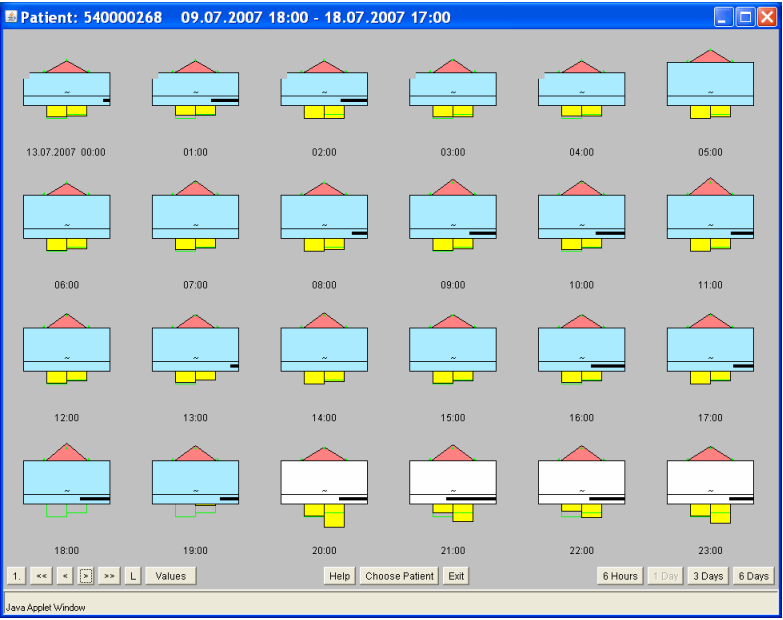
\includegraphics[width=0.6\textwidth]{fig/litteratursok/mange_glyphs.PNG}
  \caption{Bruk av grafiske elementer i VIE-VISU \citep{rind2011interactive}.}
\label{fig:mange_glyphs}
\end{figure}

\begin{figure}[H]
  \centering
    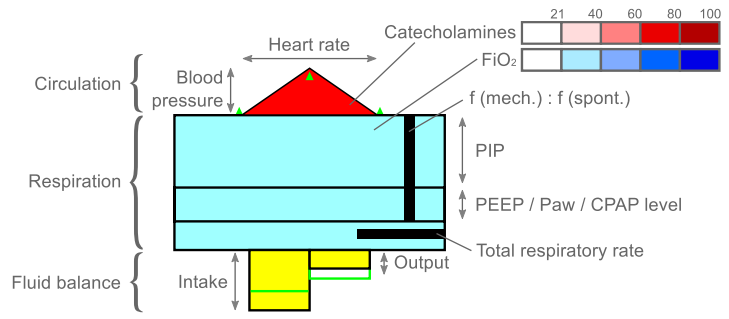
\includegraphics[width=0.6\textwidth]{fig/litteratursok/detalj_glyph.PNG}
  \caption{Bruk av farger i VIE-VISU \citep{rind2011interactive}.}
\label{fig:detalj_glyph}
\end{figure}


\section{Representasjon av legemiddelkunnskap}
Generell legemiddelinformasjon er i stor grad tilgjengelig på Internett. Noe av det som kan skille Mine Medisiner fra eksisterende systemer er personlig og situasjonsavhengig informasjon. For at Mine Medisiner skal være nyskapende bør det kunne svare på spørsmål som krever omfattende søk i eksisterende kilder, eller ekspertise fra helsepersonell, å besvare. For at en ferdig implementasjon av Mine Medisiner skal kunne realiseres må den bygge på en representasjon av legemiddelkunnskap. Vi gjorde et litteratursøk for å undersøke mulighetene for å lage en representasjon av legemiddelkunnskap som egner seg for Mine Medisiner.

For å representere legemiddelkunnskap kan man lage en ontologi. Begrepet ontologi har sin opprinnelse fra filosofien og betegner læren om det som finnes. Innenfor informasjonsteknologi brukes begrepet ontologi for å betegne en formell representasjon av begreper innenfor et domene, og hvordan disse begrepene relaterer til hverandre \citep{barrysmithOnto}.

Et kompetansespørsmål er et typisk spørsmål som man ønsker at en ontologi skal kunne besvare. Kompetansespørsmål definerer ontologiens krav ved at de angir hvilke spørsmål ontologien skal være i stand til å besvare \citep{Gangemi, Fox}.

Kompetansespørsmål kan bli brukt til å vurdere hvor god dekning en ontologi har. Dette gjøres ved at man måler hvor stor prosentandel av kompetansespørsmålene som ontologien er i stand til å besvare. For at kompetansespørsmålene skal gi en god indikasjon på dekningen til ontologien må man sørge for at kompetansespørsmålene i seg selv har god dekning \citep{Rao}.

\begin{table}[H]
    \centering
    \begin{tabularx}{\textwidth}{|X|}
    \hline
        \textbf{Kompetansespørsmål til Mine Medisiner sin ontologi}
        \begin{enumerate}
            \item For enhver effekt skal det være mulig å spørre om et legemiddel eller en kombinasjon av legemidler kan gi denne effekten
            \item For hvert legemiddel skal det være mulig å spørre om legemiddelinformasjon. Legemiddelinformasjon inkluderer:
            \begin{itemize}
                \item Indikasjoner
                \item Mulige bivirkninger
                \item Dosering
            \end{itemize}
            \item For hver legemiddelkombinasjon skal det være mulig å spørre om:
            \begin{itemize}
                \item Interaksjoner  mellom noen av legemidlene i legemiddelkombinasjonen
                \item Overlapp i effekt  mellom noen av legemidlene i legemiddelkombinasjonen
                \item Motvirkende effekter mellom noen av legemidlene i legemiddelkombinasjonen
                \item Om noen av legemidlene i legemiddelkombinasjonen er generiske
            \end{itemize}
            \item Det må være mulig å spørre om indikasjoner, bivirkninger og interaksjoner er relevant for en spesiell pasientgruppe (aldersgruppe, kjønn, livssituasjon o.s.v.) 
        \end{enumerate} \\
    \hline
    \end{tabularx}
    \caption{Kompetansespørsmål til Mine Medisiner sin ontologi}
    \label{tab:kompspm}
\end{table}


En gruppe med fire studenter(HAFE), som tok faget TDT4215 Web Intelligence våren 2015, laget en enkel legemiddelontologi som er hardkodet til å fungere for noen av personene som er presentert i delkapittel~\ref{sec:personae}. Ontologien er i stand til å besvare kompetansespørsmålene til Mine Medisiner sin ontologi (se tabell~\ref{tab:kompspm}), men den inneholder mange forenklinger. Disse forenklingene gjør at ontologien ikke er i stand til å modellere virkeligheten på en tilstrekkelig måte for en ferdig versjon av Mine Medisine. Sluttraporten til HAFE-prosjektet ligger i vedlegg~\ref{HEFE}.

En vanlig kilde til feil i ontologier for legemidler er at virkningen av legemiddelet bare knyttes til enkeltmolekyler av virkestoffer. Virkemidler er viktig for hvilken effekt legemidler får, men også hvilken form (tablett, veske, inhalator) legemiddelet er i, hvilken dose som tas, hvilke andre legemidler som tas, med mer. \acrfull{dron} er en ontologi som tar hensyn til at det er flere faktorer som påvirker effekten av legemidler. \acrshort{dron} har som mål at det skal bli mulig å gjøre spørringer på virkestoff, effekt av legemiddel og den terapeutiske klassen legemiddelet tilhører \citep{HoganTowards, BuildingDrugOntology}.

\acrshort{dron} er avansert, komplekst og muliggjør resonnering, men for at den skal være nyttig for Mine Medisiner må den tilpasses noe i struktur og innhold. \acrshort{dron} må fylles med norske kliniske terminologier (ordnett, \acrshort{icd}10, \acrshort{mesh} og annet fra finnkode.no), og tilpasses så den kan besvare kompetansespørsmålene til Mine Medisiner sin ontologi, se tabell~\ref{tab:kompspm}. 

\acrfull{dideo} er en planlagt ontologi som skal basere seg på \acrshort{dron}, \acrfull{dio} og \acrfull{dinto}. \acrshort{dio} og \acrshort{dinto} er to ontologier for legemiddelinteraksjoner. Fordi \acrshort{dideo} vil inneholde informasjon om interaksjoner vil den kunne besvare flere av kompetansespørsmålene til Mine Medisiner sin ontologi enn \acrshort{dron}. \acrshort{dideo} er imidlertid ikke utviklet enda \citep{brochhausen2014towards}.

KEGG DRUG er en legemiddelinformasjonskilde for godkjente legemidler i Japan, USA og Europa. Legemiddelinformasjonen er strukturert ut i fra kjemiske strukturer og annen informasjon på molekylnivå. Interaksjoner til legemidler som selges på resept i Japan har blitt funnet og lagt til i KEGG DRUG ved å analysere alle pakningsvedlegg ved hjelp av naturlig språkprosessering\footnote{Natural language processing (NLP) er et felt innen informatikk, kunstig intelligens og datalingvistikk som handler om samspillet mellom datamaskiner og menneskelige språks}. Interaksjonene er prosessert og klassifisert i hierarkier av kjemiske strukturer og \acrshort{atc}-koder. Hierarkiene gjør at nettverket av interaksjoner kan analyseres på forskjellige granularitetsnivåer. \acrshort{kegg} DRUG gjør det mulig å søke etter kjente interaksjoner, og forutse potensielle interaksjoner mellom reseptbelagte legemidler i Japan \citep{takarabe2011network}.

For å lage en legemiddelontologi må det ligge en klinisk terminologi til grunn, slik at de som samarbeider som utviklingen har en felles forståelse av konvensjonene for å representere klinisk kunnskap. 

\section{Klinisk terminologi}
Klinisk terminologi betegner ord, uttrykk og begreper brukt i helsevesenet. En utfordring med kilder til legemiddelinformasjon, blant annet pakningsvedlegg, er bruken av vanskelige fagterminologier. I Mine Medisiner er det forsøkt å gjøre innholdet forståelig for folk uten helsefaglig bakgrunn, uten at det skal gå ut over kompletthet eller korrektheten til innholdet. 

Det er både språklige og pragmatiske utfordringer ved å utvikle en medisinsk terminologi. Språket må være riktig og høres naturlig ut for en som snakker språket, og innholdet må passe til oppgavene som skal utføres. En utfordring er at medisinsk terminologi kan avvike fra det som virker logisk eller språklige konvensjoner tilsier, ved at betydningen ikke er ordrett  \citep{rector1999clinical}.

Konsensus omkring medisinske begreper og klassifiseringer har vist seg å ikke alltid være mulig blant klinikere. Begrepet kan ha vidt forskjellig betydning på ulike steder. Dette gjør at lokale tilpasninger er nødvendig for klinisk terminologi. 

Eksisterende medisinske kodeverk, f.eks \acrshort{icd}-10, har en kompleks struktur. Det kan være en utfordring å utvikle kliniske terminologier som tar hensyn til eksisterende kodeverk. En annen utfordring er å holde terminologien oppdatert. En klinisk terminologi må være dynamisk fordi ny informasjon og flere detaljer og relasjoner stadig oppstår. 

Det er viktig å spesifisere hvilke oppgaver terminologien skal støtte, og hvilke aktiviteter og brukere som skal ha nytte av den. En altomfattende terminologi som skal tilfredsstille behovet til både forskere, produsenter, forsikringsselskap, staten og helsetjenesten, er vanskelig å få til. En løsning kan være å lage flere typer terminologier til forskjellig bruk, med SNOMED RT\footnote{SNOMED RT: SNOMED reference Terminology} som referanseterminologi \citep{spackman1997snomed}. 




\chapter{Utviklingsmetoder} \label{chap:utviklingsmetoder}

De forrige kapittelene presenterte en plan for forskningen og knyttet dette opp mot hva som allerede er gjort, gjennom et litteraturstudie. Dette kapittelet handler om utviklingsmetodene benyttet for å lage en prototype av Mine Medisiner. Med forskningsspørsmålet i tankene, var det åpenbart at vi måtte rette utviklingen mot pasienter. Vi valgte en brukersentrert utviklingsprosess, jf. delkapittel~\ref{sec:brukersentrert}. Dette er en utviklingsfilosofi som aktivt involverer brukere gjennom utviklingsprosessen. 

En oversikt over hvilke utviklingsmetoder vi har brukt, og hensikten med de ulike metodene er vist i tabell \ref{tab:utviklingsmetodene}.

\begin{table}[H]
    \centering
    \begin{tabular}{ | l | p{7cm} | }
      \hline
      \textbf{Metode} & \textbf{Hensikt} \\ \hline
      Personae & Bli kjent med målgruppen \\ \hline
      User Stories & Fortså brukeren og utforske samspillet mellom brukeren og systemet \\ \hline
      Workshop & Utveklse idéer og meninger \\ \hline
      Semistrukturert intervju & Samle informasjon og forstå legemiddelfagfeltet \\ \hline
      Prototyping & Teste designmuligheter og få tilbakemeldinger som gjorde det mulig å lage en bedre prototype \\ 
      \hline
    \end{tabular}
    \caption{Oversikt over utviklingsmetodene som ble brukt}
    \label{tab:utviklingsmetodene}
\end{table}


\section{Personae}
Personae er personprofiler utviklet for å beskrive målgruppen til en tjeneste. Personae er et nyttig virkemiddel for å bli kjent med målgruppen og for å se for seg konkrete brukseksempler. 
\section{User Stories}
User stories beskriver hvordan brukere ønsker å interagere med et system. Med utgangspunkt i personae beskrives tjenesten fra brukerenes perspektiv. Formålet med user stories er å forstå hvordan brukerene møter systemet og å verifisere at brukerenes behov er tatt hensyn til.

User stories kan presenteres på flere måter, blant annet som story boards og tekstbeskrivelser. Et story board illustrerer en situasjon hvor et system blir benyttet. Den vanligste måten å lage story boards på er i form av tegneseriestriper. Story boards bør lages slik at hvem som helst kan forstå dem. 

\section{Workshop}
En workshop er en arbeidsform med vekt på samhandling mellom deltakerne. Deltakerne utveksler meninger og ideer for å komme frem til et felles resultat. Dette resultatet kan være abstrakt (f.eks. økt innsikt i et tema) eller konkret (f.eks. en prototype).

En workshop kan bestå av flere deler, blant annet oppgaver eller diskusjoner. Det kan variere hvorvidt delene skal utføres individuelt av hver enkelt deltaker, eller om de skal utføres sammen av gruppen. En workshop kan tilpasses underveis.

\section{Semistrukturert intervju}
Et intervju er en samtale mellom to eller flere personer, hvor en intervjuer stiller spørsmål, og et intervjuobjekt svarer. Målet med et intervju er å samle informasjon. Mye av informasjonen får man gjennom hva intervjuobjektet sier, men det er også verdifull informasjon i intervjuobjektets kroppsspråk og stemmebruk. 

Et semistrukturert intervju har gjerne en overordnet plan med samtaleemner, men samtalen drives videre av interessante tema som dukker opp underveis i intervju. En fordel med semistrukturerte intervjuer er at de kan tilpasses underveis ved å be om forklaringer, stille oppfølgingsspørsmål eller utforske nye emner som dukker opp. Denne typen tilpasning kan bidra til å forstå intervjuobjektet bedre og til å oppmuntre intervjuobjektet. Det er viktig å finne en balansegang da for mange oppfølgingsspørsmål kan gjør at intervjuobjektet føler seg utilpass \citep{Seidman}.

Bruk av personprofiler i et intervju kan være et nyttig hjelpemiddel for å unngå personlige spørsmål. Istedenfor å stille spørsmål knyttet til intervjuobjektets situasjon knytter man spørsmålene opp til personprofiler spesielt utviklet for dette formålet.

\section{Prototyping}
Prototyping er brukt som utviklingsmetode, og er presentert i delkapittel~\ref{sec:prototyping}.
\chapter{Utvikling av prototype}\label{chap:utvikleprototype}

Utviklingsprosessen startet med å samle inn informasjon for å forstå brukerne, deres behov og legemiddeldomene. Dette ble gjort ved hjelp av personae, user stories, workshop og intervju. Videre utviklet vi en papirprototype som ble testet for å brukes i videre utvikling. Sluttproduktet av utviklingsprosessen var en digital prototype av Mine Medisiner. I dette kapittelet er arbeidet frem mot denne prototypen beskrevet.
Prosessen er kan oppsummeres i følgende punkter
\begin{enumerate}
\item Samle informasjon om legemiddeldomenet og pasienters behov for legemiddelkunnskap (delkapittel~\ref{sec:personae} og~\ref{sec:workshopFarm}). 
\item Bruke informasjonen til å utvikle en papirprototype for Mine Medisiner (delkapittel~\ref{sec:workshopDesign}). 
\item Teste papirprototype for Mine Medisiner (delkapittel~\ref{sec:firstBrukertest})
\item Bruke tilbakemeldingene fra papirprototypetesten til å lage en digital prototype (delkapittel~\ref{sec:digitalPrototype}). 
\end{enumerate}


\section{Personae}\label{sec:personae}
Målet med bruk av personae var å bli kjent med målgruppen til Mine Medisiner. 

Personae som ble brukt i prosjektet ble utviklet av biveileder og farmasøyt, Janne sund. Hun utviklet fem personae som illustrerer ulike typer pasienter i målgruppen. For å dekke størst mulig del av målgruppen er personae forskjellige, men alle har trekk som går igjen hos mange pasienter.

\subsection{Lillian 27 år}
Lillian, se vedlegg~\ref{chap:lillian}, går fast på legemidler mot epilepsi, og prøver å bli gravid. Pasientgruppen Lillian tilhører er veldig opptatt av legemiddelinformasjon. Lillian har tatt legemidlene over lang tid, og har opparbeidet seg kunnskap om egne legemidler. Nå som hun prøver å bli gravid befinner hun seg i en ny situasjon, som gjør at hun har behov for annen informasjon enn tidligere.

\subsection{Lars 57 år}
Lars tok ingen legemidler før han nylig fikk et større hjerteinfarkt, se vedlegg~\ref{chap:lars}. Lars tilhører en pasientgruppe som har et stort informasjonsbehov. Pasienter som får hjerteinfarkt for første gang er ofte ukjent med å stå på faste legemidler. Etter hjerteinfarkt er det vanlig å få legemidler for å forebygge et nytt infarkt. Ofte skal pasienten stå på disse legemidlene resten av livet.

\subsection{Kåre 77 år}
Kåre har flere sykdommer som er typisk for sin aldersgruppe, se vedlegg~\ref{chap:kaare}. Han har diabetes, går på blodfortynnende, og tar smertestillende regelmessig. Kåre er klar over hvilke utfordringer han har med helsen, men klarer ikke å knytte legemidlene til problemene sine.

\subsection{Håkon 83 år}
Håkon har hatt to \acrshort{tia}-anfall det siste halvannet året, se vedlegg~\ref{chap:haakon}. I likhet med mange andre som har hatt \acrshort{tia}-anfall er Håkon bekymret for å få nye \acrshort{tia}-anfall eller slag.

\subsection{Klara 87 år}
Klara har tatt legemidler fast i mange år, se vedlegg~\ref{chap:klara}. Blant eldre er det ikke uvanlig å ta legemidler fast, og å ha gjort dette over lang tid. Klara bor i en omsorgsbolig, men håndterer legemidlene sine selv. Hun har stor tiltro til sin lege og tør ikke tvile på legemidlene han har forskrevet.  

\section{Workshop med farmasøyter} \label{sec:workshopFarm}
Hovedmålet for workshopen var å få en forståelse av pasienters behov for informasjon om legemidler. 

Vi hadde to delmål:
\begin{enumerate}
\item Tilegne oss domenekunnskap
\item Utforske måter å presentere legemiddelinformasjon til pasienter
\end{enumerate}

To farmasøyter ble rekruttert for å delta i workshopen. To farmasøyter er ikke et representativt utvalg, men som et utgangspunkt for å utforske legemiddeldomenet ble det ansett for å være tilstrekkelig. 

Den første farmasøyten (farmasøyt 1) var klinisk farmasøyt. En klinisk farmasøyt jobber med pasienter på sykehuset, vurderer legemiddelbehandlingen og utfører andre oppgaver relatert til pasienters legemiddellister. Den andre farmasøyten (farmasøyt 2) jobbet bak disken på sykehusapoteket. Denne jobben går ut på å hjelpe kunder i apoteket med deres legemiddellister og resepter. 

Farmasøytene ble informert om prosjektet i forkant, med mål om at de skulle få et forhold til problemområdet, samt sikre at de gav gjennomtenkte svar. Dette så ut som det fungerte godt da begge farmasøytene var villig til å bidra ytterligere. De viste også interessere for å bli oppdatert på utviklingen i masteroppgaven.

Farmasøytene som deltok i workshopen hadde samme utdanning, selv om de hadde forskjellige roller i sykehusapoteket. At farmasøytene hadde ulike roller var et bevisst ønske for å få en bredere tilnærming til domenet.

Svar fra farmasøyter samsvarer ikke nødvendigvis med hva pasienter ville svart, men de kan ha bedre innsikt i legemiddelrelaterte spørsmål enn mange pasienter fordi de interagerer med målgruppen på daglig basis. Farmasøytene har med stor sannsynlighet jobbet med flere datasystemer på jobb, noe som kan være nyttig når avgjørelser om funksjonalitet, og hvilken informasjon som gir nytte, skal tas. 

Det er mulig at det ble stilt ledende spørsmål eller at farmasøytene på annen måte ble påvirket under workshopen. Farmasøytenes oppfatning av oss og prosjektets hensikt kan ha påvirket svarene de gav. Det er viktig å skape tillit og å fremstå nøytral når man leder en workshop, men det er vanskelig å vurdere oppnåelsen av dette. Selv om vi prøvde å fremstå som nøytrale vil det være en mulig at deltakerne svarte det de trodde vi ville høre eller at Hawthorne-effekten\footnote{Hawthorne-effekten er når noens adferd endres fordi de blir studert. Les mer: \url{https://snl.no/Hawthorneeffekten}} har spilt en rolle. Farmasøytene kan ha prøvd å fremstille arbeidshverdagen sin mer spennende enn den er, eller fortalt ting som egentlig ikke har skjedd. 

\subsection{Utførelse}

\begin{figure}[H]
    \centering
    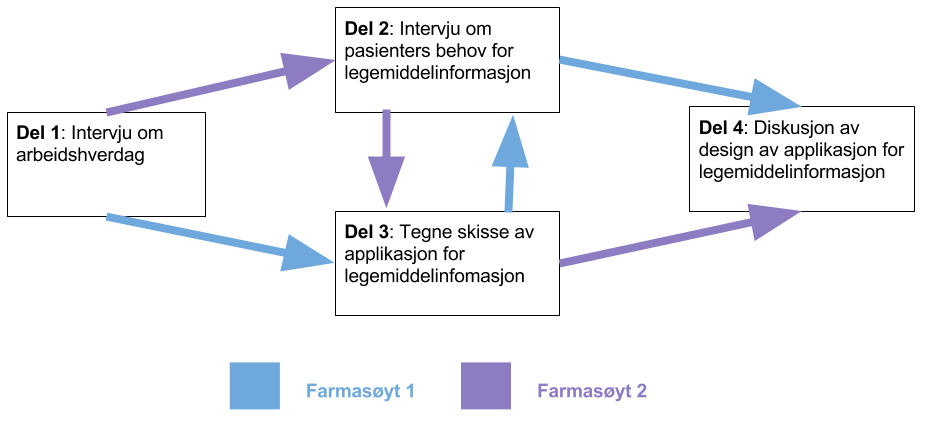
\includegraphics[width=1\textwidth]{fig/utviklingAvPrototype/1stWorkshop.png}
    \caption{flytdiagram som illustrerer rekkefølgen utførelsesdelene i workshopen ble utført.}
    \label{fig:1stWorkshop}
\end{figure}

Workshopen besto av fire deler. De tre første delene var individuelle. I den første delen fortalte farmasøytene om sine arbeidsrutiner. Den andre delen var et intervju om legemiddelinformasjon. I del tre fikk farmasøytene en designoppgave. I den siste delen diskuterte farmasøytene designoppgaven fra del tre i fellesskap. 

Det var sannsynlig at svarene i utføringsdelene av workshopen ville påvirke hverandre. For å se om intervjuet påvirket designoppgaven eller om designoppgaven påvirket intervjuet, utførte vi del to og del tre i forskjellig rekkefølge på de to farmasøytene. Den første farmasøyten hadde intervju før designoppgaven, mens den andre farmasøyten gjorde oppgavene i motsatt rekkefølge. Figur~\ref{fig:1stWorkshop} viser et flytdiagram som illustrerer de ulike delene workshopen bestod av, og rekkefølgen de ble utført i.

De to første delene av workshopen ble utført som semistrukturerte intervjuer. Et semistrukturert intervju ble brukt for å kunne tilpasse samtalen til den enkelte deltaker.

I det første intervjuet ble deltakerne bedt om å beskrive sin daglige arbeidsrutine og hvordan de samhandler med pasienter. Dette ble gjort for å bli kjent med farmasøytene, og for å bedre forstå deres tankegang i de følgende delene av workshopen. 

I det andre intervjuet var spørsmålene relatert til forståelse av pasientenes behov for informasjon. En detaljert beskrivelse av intervjuet finnes i vedlegg~\ref{chap:interview1stWorkshop}.

I den tredje delen av workshopen ble deltakerne spurt om å lage en skisse av en applikasjon som skulle presentere legemiddelinformasjon til en pasient. For å kunne få en forståelse for valgene som ble tatt underveis ble farmasøytene instruert til å tenke høyt mens de tegnet. De ble også spurt om å spesifisere hvilken informasjon de trodde var nyttig for pasienter og om det eventuelt var informasjon de mente ikke burde vises.

Den fjerde delen besto av en diskusjonsdel. Deltakerne ble spurt om å presentere sine design fra del tre, for hverandre. Deltakerne diskuterte begge løsningene. Hovedpunktene var forskjeller i måten de presenterte informasjon på, og hvilken informasjon de hadde valgt å ta med. 

\subsection{Resultat}
Workshopen viste at det var behov for at \textit{personlig} legemiddelinformasjon blir lettere tilgjengelig for pasienter.

Målene for workshopen var delt inn i to delmål.  
\begin{enumerate}
\item \textbf{Tilegne oss domenekunnskap:}\\
Det er vanskelig å vurdere oppnåelsen av et ikke-målbart mål som å tilegne seg domenekunnskap. Vi mener at workshopen, spesielt intervjudelen, gav oss innsikt i domenet, og  anser derfor dette målet for oppnådd.

\item \textbf{Utforske måter å presentere legemiddelinformasjon til pasienter:}\\
Designoppgaven utforsket hvordan farmasøytene mente det ville være mulig å fremstille informasjon for pasienter. Farmasøytene utførte oppgaven hver for seg, noe som resulterte i ulike muligheter å presentere informasjon på.
\end{enumerate}

Resultatet skal brukes som et utgangspunkt for videre arbeid mot en prototype. 

\section{Workshop for å lage første prototype} \label{sec:workshopDesign}
Målet med denne workshopen var å utvikle en papirprototype for Mine Medisiner. Workshopen ble utført med hjelp og støtte fra Capgemini sin user experience-avdeling.

\subsection{Forarbeid}
Som forarbeid til workshopen laget vi en liste med funksjonelle krav som skal inkluderes i prototypen. En user story basert på en persona, se vedlegg~\ref{chap:kaareHistorie}, ble utviklet for å verifisere at kravene dekket denne personen sine behov. User storyen var med på å avdekke nye krav som ble lagt til i listen. 

Den totale listen med krav ble rangert, basert på to faktorer: \textit{hvor viktig kravet er for applikasjonen} gav høyere rangering, og \textit{hvor vanskelig det vil være å implementere kravet} gav lavere rangering. Det var veldig viktig at systemet inneholdt informasjon om bivirkninger og interaksjoner siden det var en del av forskningsspørsmålet.
Noen av kravene er ikke direkte knyttet til interaksjoner og bivirkninger, men støtter hovedfunksjonaliteten og  bidrar til helheten i systemet. Den endelige listen med funksjonelle krav til papirprototypen i rangert rekkefølge er gitt i tabell~\ref{tab:krav}. 

\begin{table}[H]
    \centering
    \begin{tabular}{|c|p{9cm}|}
     \hline
     \textbf{Rangering} &         \textbf{Funksjonelle krav som skal inkluderes i prototypen} \\ \hline
     1 & Innlogging \\  \hline
     2 & Vise personlig legemiddelliste  \\  \hline
     3 & Legge til legemiddel i personlig legemiddelliste \\  \hline
     4 & Vise mulige bivirkninger for legemidlene \\  \hline
     5 & Vise mulige interaksjoner mellom legemidlene \\  \hline
     6 & Vise hva legemidlene er ment å behandle \\  \hline
     7 & Fjerne legemiddel fra personlige legemiddelliste \\  \hline
     8 & Advarsel om å kontakte lege når det er passende \\  \hline
     9 & Kunne tilpasse hvor mye informasjon som er synlig \\  \hline
     10 & Indikere hvor alvorlig en bivirkning er \\  \hline
     11 & Indikere hvor vanlig en interaksjon er \\  \hline
     12 & Støtte for å legge inn personlige notater \\  \hline
     13 & Støtte for å inkludere ikke-reseptbelagte legemidler i legemiddellisten \\  \hline
     14 & Vise bilde av hvert legemiddel \\  \hline
     15 & Vise utløpsdato for hvert legemiddel \\  \hline
     16 & Støtte for å rapportere opplevde bivirkninger  \\  \hline
     17 & Indikere når legemidler har samme virkestoff \\  \hline
     18 & Vise advarsel for mat, drikke og helsekostprodukter som ikke bør kombineres med legemidler \\  \hline
     19 & Vise advarsel dersom legemiddelet påvirker evnen til å operere tungt maskineri, f.eks. kjøre bil \\  \hline
     20 & Vise hva langtidsvirkningen av å ta legemidlene er \\  \hline
     \end{tabular}
    \caption{Tabell over kravene innhentet ved Workshoppen med farmasøyter }
    \label{tab:krav}
\end{table}

\subsection{Utførelse}
Under workshopen gikk vi gjennom kravene etter tur og diskuterte hvordan vi kunne oppfylle dem. Noen krav var vanskeligere enn andre å oppfylle. I det følgende er diskusjonen om hvordan vi på best mulig måte kunne vise interaksjoner mellom legemidler og bivirkningene til legemidlene i legemiddellisten utdypet. 

\subsubsection{Vise mulige interaksjoner mellom legemidlene}
Vi diskuterte to forskjellige måter å vise interaksjoner på: en tekstlig beskrivelse og en grafisk fremstilling.

I en tekstlig beskrivelse ville hver interaksjon vært på formen “legemiddel A og legemiddel B kan forårsake interaksjon C”. Dette ligner mye på resultatlisten på interaksjoner.no, se figur~\ref{fig:interaksjoner}. Istedenfor å bruke \acrshort{atc}-koder i listen over interaksjoner ville vi brukt de norske handelsnavnene på legemidlene. Dette ville gjort det lettere for brukerne av systemet å se hvilke legemidler som er involvert i interaksjonene. 

\begin{figure}[H]
    \centering
    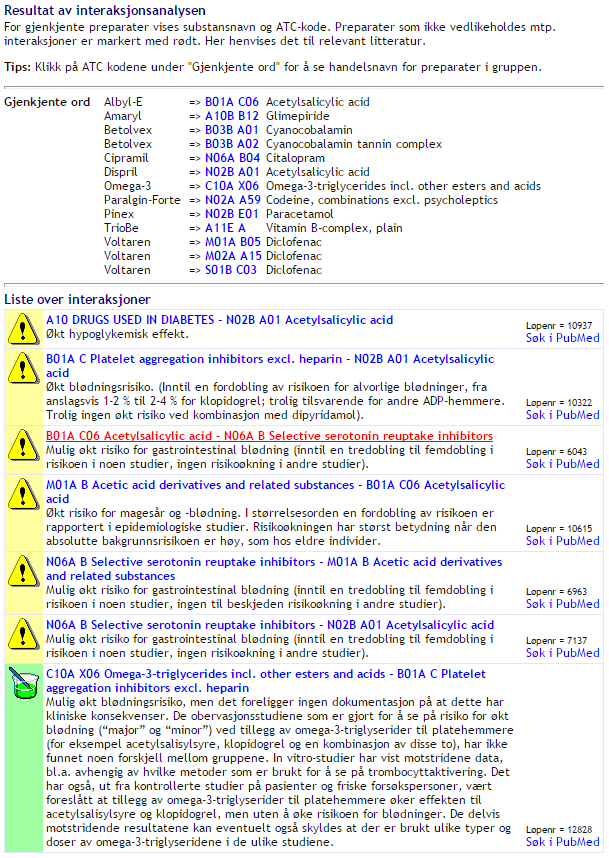
\includegraphics[width=1\textwidth]{fig/utviklingAvPrototype/interaksjoner.PNG}
    \caption{Interaksjoner.no med søkeresultatet av å skrive inn Kåre sin legemiddelliste: Albyl-E, Voltaren, Dispril, Pinex, Amaryl Cipramil, Paralgin forte, Betolvex, TrioBe og Omega-3}
    \label{fig:interaksjoner}
\end{figure}

For papirprototypen bestemte vi oss for en grafisk fremstilling av interaksjonene. Det er to typer noder der den ene representerer legemidler, og den andre representerer effekt av interaksjoner. Kantene som kobler nodene sammen indikerer hvilke legemidler som hører til de ulike effektene av interaksjoner. Et eksempel er vist i figur~\ref{fig:grafInteraksjon}.

\begin{figure}[H]
    \centering
    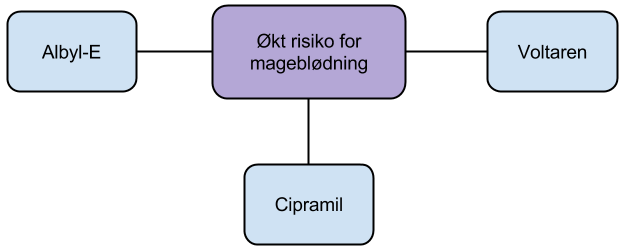
\includegraphics[width=0.8\textwidth]{fig/utviklingAvPrototype/grafPrototype.png}
    \caption{Interaksjoner representert som en graf. Albyl-E, Cipramil og Voltaren kan sammen gi økt risiko for mageblødning.}
    \label{fig:grafInteraksjon}
\end{figure} 

En grafisk fremstilling av interaksjoner kan ha ekstra funksjoner for å utforske grafen. Eksempler på dette er zooming, flyttbare noder og mulighet til å utheve bestemte deler av grafen. Vi valgte å ikke inkludere dette i papirprototypen. 

Under workshopen diskuterte vi å legge til informasjon om bivirkninger, overlappende effekter og motvirkende effekter i interaksjonsgrafen. Etter å ha forsøkt dette for noen legemiddelsituasjoner fant vi ut at dette ville resultere i svært store og komplekse grafer. Vi valgte derfor å kun legge til motvirkende effekter i interaksjonsgrafen.  

\subsubsection{Vise mulige bivirkninger for legemidlene}
Vi vurderte flere muligheter for å vise bivirkninger: inkludere bivirkninger i interaksjonsgrafen, vise bivirkninger i en ordsky, vise bivirkninger som fliser og å ha en søkefunksjon for å finne bivirkninger.  

En grafisk fremstilling av bivirkninger blir veldig stor og kompleks fordi de fleste legemidler har mange mulige bivirkninger. En måte å gjøre en slik graf mindre er ved å bare ta med de mest vanlige bivirkningene. Vi gjorde et forsøk på å lage en graf for Kåre, se vedlegg~\ref{chap:kaare}, som inneholdt interaksjoner og de vanligste bivirkningene for hans legemidler. Denne grafen ble veldig kompleks, så idéen om grafisk fremstilling av bivirkninger ble droppet. 

Den neste idéen var å vise bivirkninger som en ordsky. Jo flere legemidler en bivirkning tilhørte, jo større ville teksten være. Vi forsøkte å lage en ordsky for bivirkningene til Kåre, se vedlegg~\ref{chap:kaare}, sin legemiddelliste, se figur~\ref{fig:ordsky}. Mange av bivirkningen til legemidlene i Kåre sin legemiddelliste gjaldt bare for ett av legemidlene i listen hans. Dette gjorde at mange ordene i ordskyen ble like store, og at det var tilfeldig hvilke ord som ble inkludert i ordskyen. Ordskyen var vanskelig å lese og å forstå fordi den var rotete. Ordskyen ble ikke like intuitiv som vi hadde håpet på, og vi gikk bort fra denne idéen.

\begin{figure}[H]
    \centering
    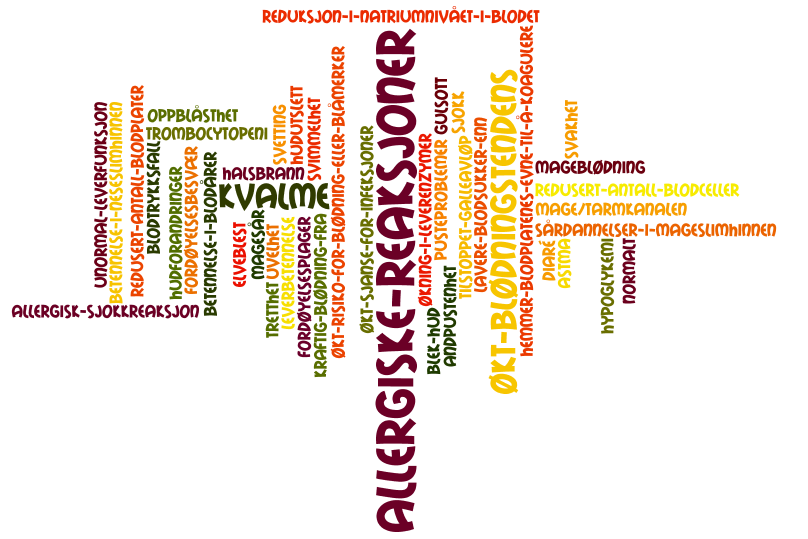
\includegraphics[width=0.8\textwidth]{fig/utviklingAvPrototype/ordsky.PNG}
    \caption{Ordsky for bivirkningene til Kåre sin legemiddelliste}
    \label{fig:ordsky}
\end{figure} 

Videre så vi på idéen om å representere alle bivirkningene for legemiddellisten ved å bruke fliser. Se figur~\ref{fig:tiles} for et eksempel på hvordan fliser for det periodiske system kan se ut. Denne måten å vise bivirkninger hadde de samme problemene som de to forrige: Antallet bivirkninger for legemiddellisten kan være veldig stort, og det er vanskelig å finne relevant informasjon når veldig mye blir presentert på en gang. Vi valgte derfor å ikke bruke fliser for å vise bivirkninger.

\begin{figure}[H]
    \centering
    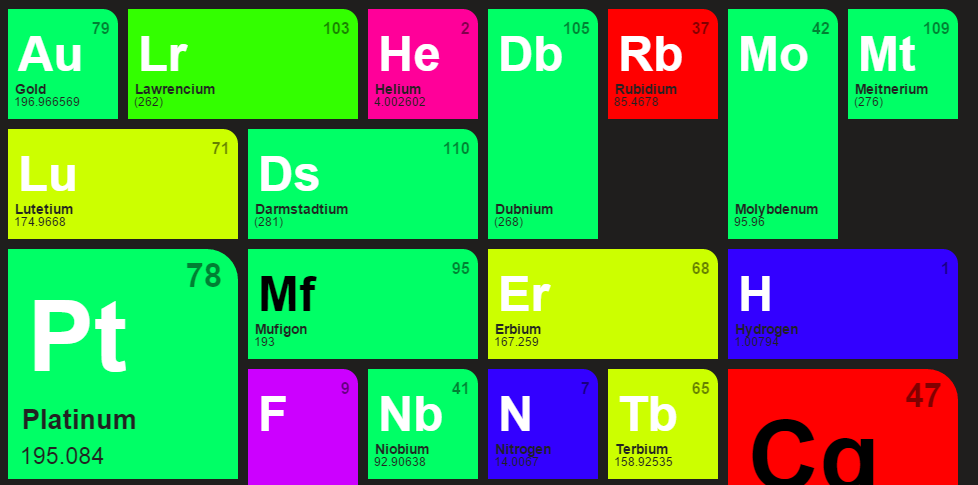
\includegraphics[width=0.8\textwidth]{fig/utviklingAvPrototype/tiles.PNG}
    \caption{Eksempel på bruk av fliser for å visualisere det periodiske system}
    \label{fig:tiles}
\end{figure} 

Den siste idéen vi vurderte var å ha en søkefunksjon for bivirkninger. I et søkefelt kunne brukerne skrive inn bivirkninger som fritekst, som for eksempel “hodepine” eller “forstoppelse”. Svaret på et slikt søk var en liste med legemidlene i legemiddellisten som har disse symptomene som bivirkning, interaksjon eller indikasjon. Denne måten å vise bivirkninger på kan unngå noceboeffekten\footnote{Nocebo (motsatt av placebo) er det at negative forventninger fører til redusert effekt av en behandling.} som ble nevnt i workshop med farmasøytene, se vedlegg~\ref{chap:interview1stWorkshop}.

\subsection{Resultat}
Resultatet av workshopen var en papirprototype for hvordan Mine Medisiner ser ut for Kåre, se vedlegg~\ref{chap:kaare}. Prototypen besto av fire sider og to pop-upvinduer: “Logg inn”-side, “Min legemiddelliste”-side, “Interaksjoner”-side, “Søk i symptomer”-side, “Symptom på interaksjon”-pop-up og “Legemiddelvisning”-pop-up. 

\pagebreak
\subsubsection{Side 1: “Logg inn”}
Det første skjermbilde brukeren presenteres for er innlogging, se figur~\ref{fig:login}. Vi bestemte oss for å bruke difi sin innlogging med høyeste autentiseringsnivå i Norge\footnote{Les mer om de ulike autentiseringsnivåene her: \url{http://eid.difi.no/nb/sikkerhet-og-personvern/informasjon-om-sikkerhetsniva}}.

\begin{figure}[H]
    \centering
    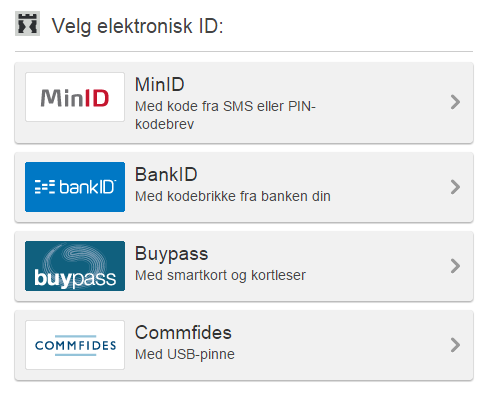
\includegraphics[width=0.8\textwidth]{fig/utviklingAvPrototype/login.PNG}
    \caption{Logg inn}
    \label{fig:login}
\end{figure} 

\subsubsection{Side 2: “Min legemiddelliste”}
Når brukeren er logget inn vises en personlig liste med legemidler, se figur~\ref{fig:legemiddellistePP}. Her kan brukeren redigere legemiddellisten sin ved å legge til eller fjerne legemidler. Hver rad inneholder navn på legemiddelet, dose, når legemiddelet skal tas og årsaken til at legemiddelet skal tas. I tillegg er det markert dersom et legemiddel har gått ut på dato. 

\begin{figure}[H]
    \centering
    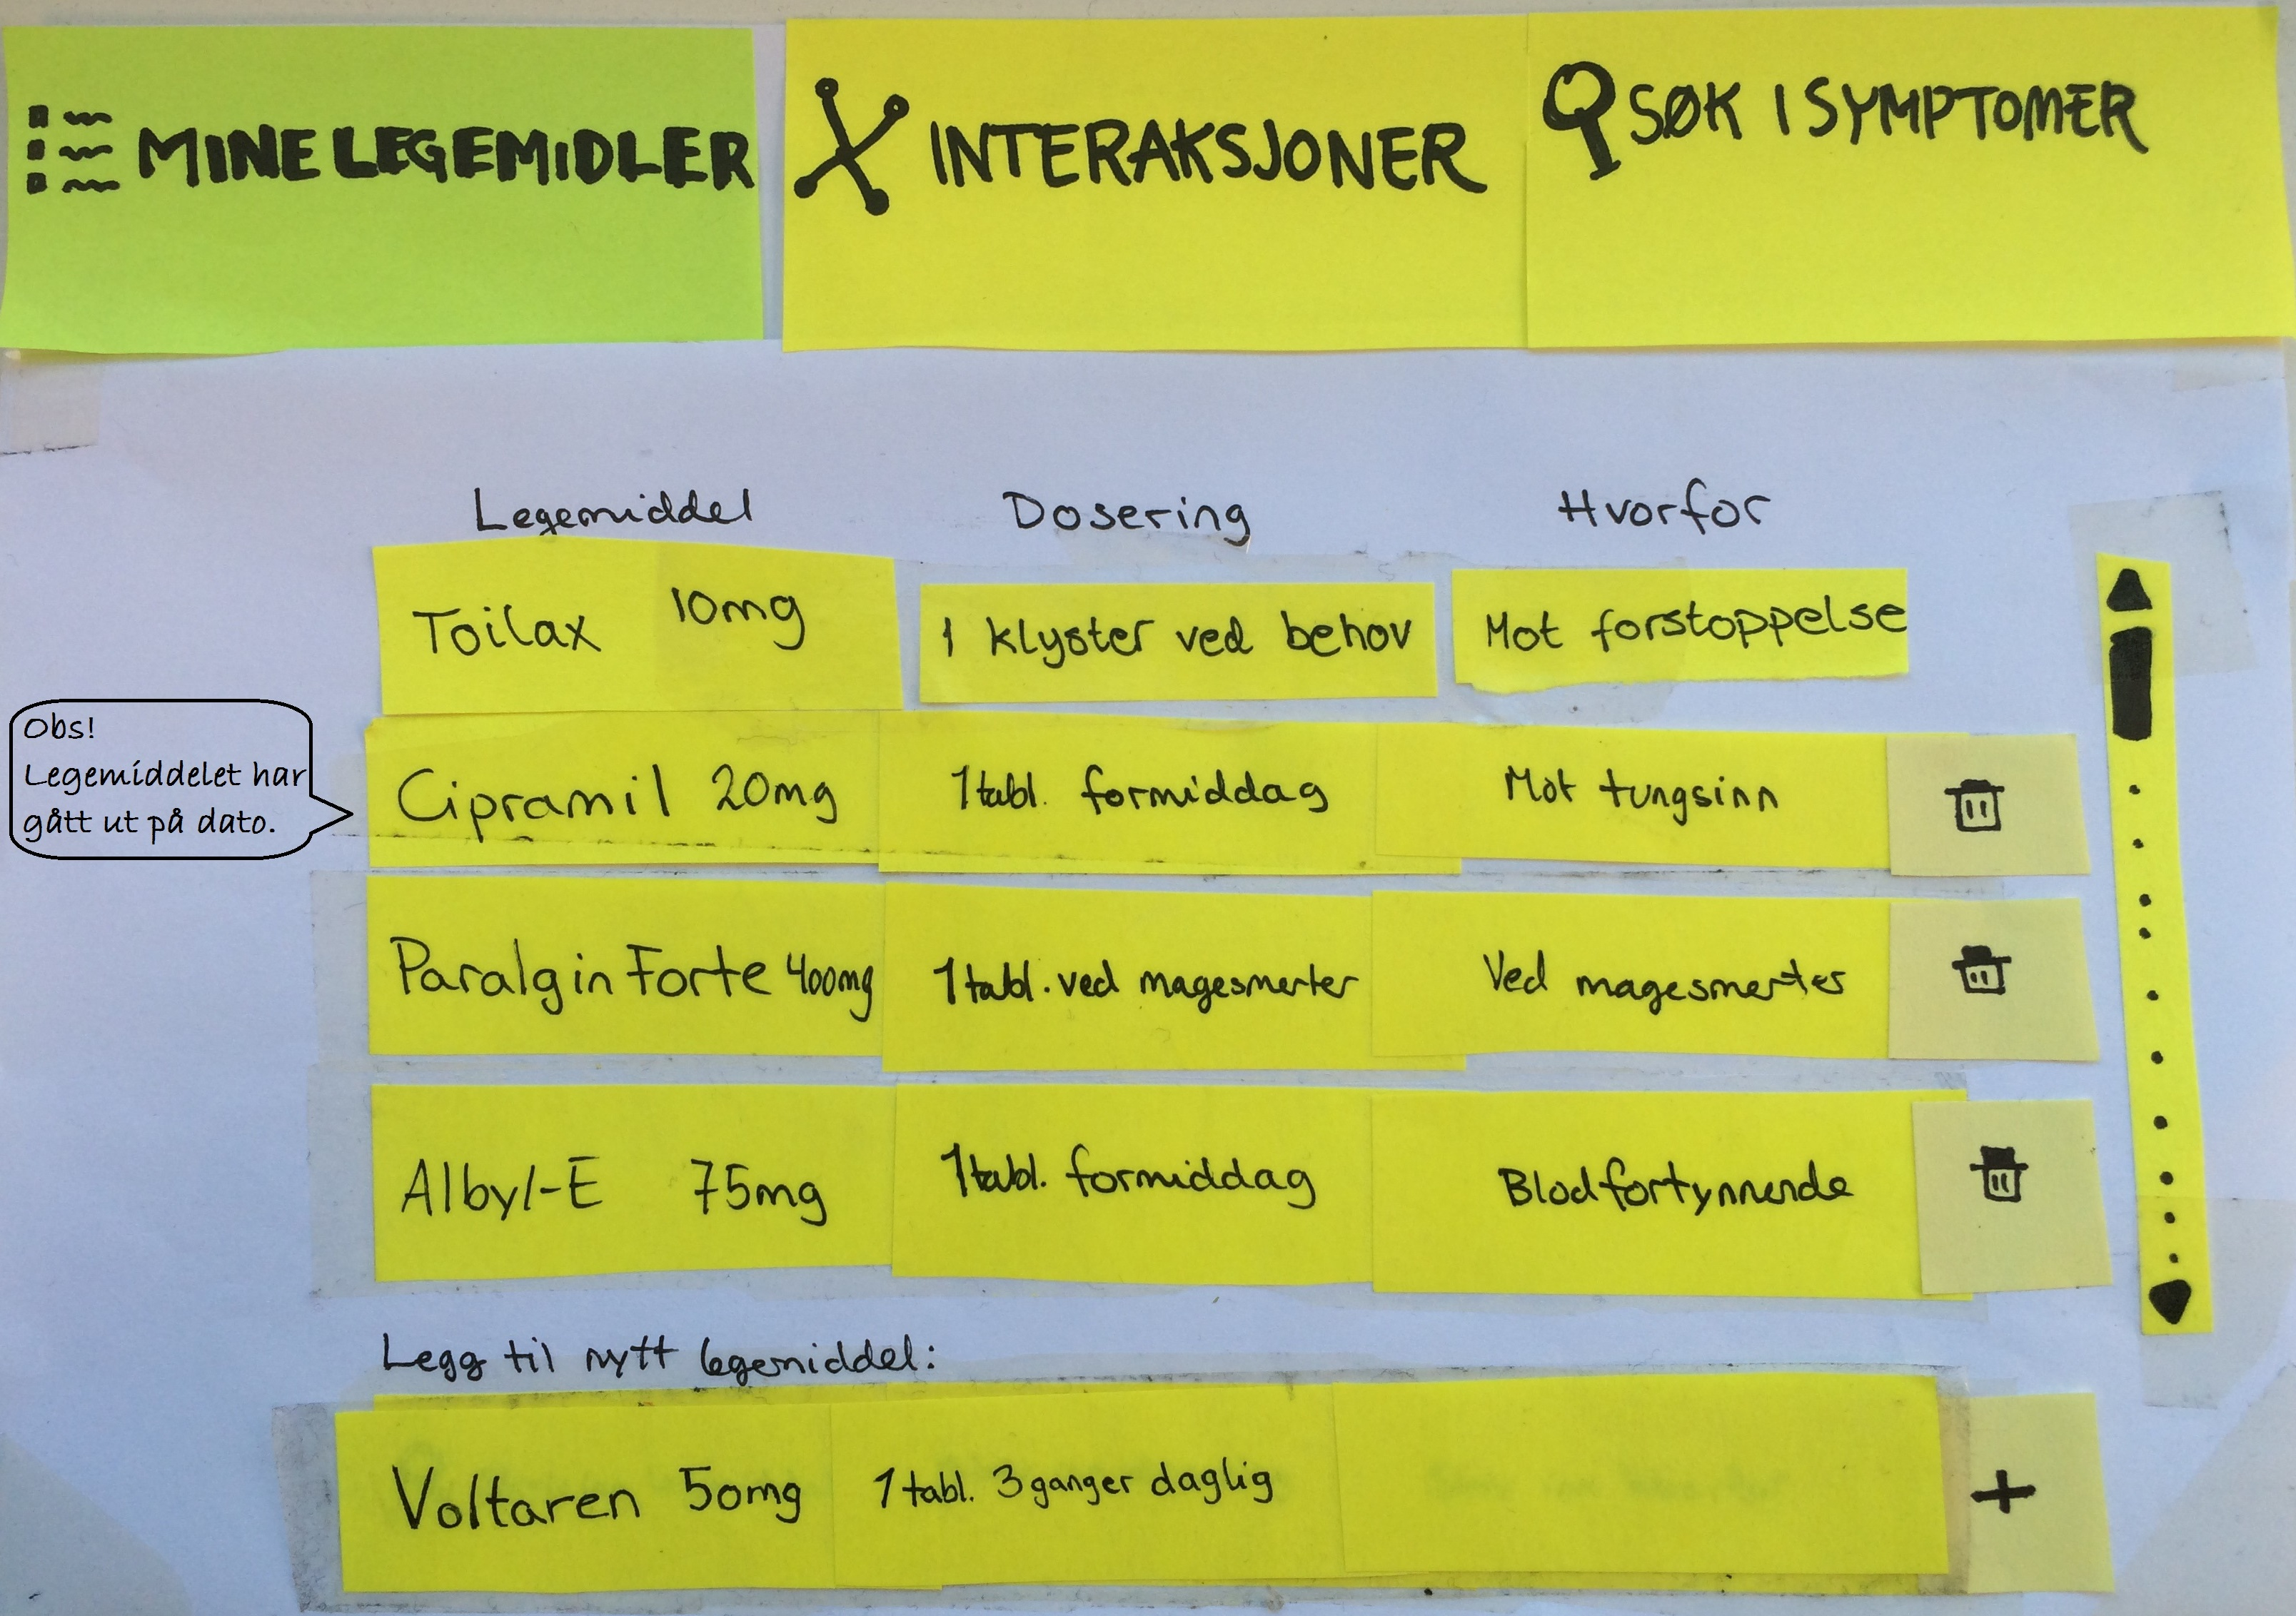
\includegraphics[width=1\textwidth]{fig/utviklingAvPrototype/mineLegemidelerPP.jpg}
    \caption{Min legemiddelliste}
    \label{fig:legemiddellistePP}
\end{figure} 

\subsubsection{Side 3: “Interaksjoner”}
Under fanen “interaksjoner” visualiseres interaksjoner relatert til den personlige legemiddellisten, som vist i figur~\ref{fig:interaksjonsgrafPP}. Legemidler som har en interaksjon kobles sammen med blå bokser som viser hva kombinasjonen av legemiddelene kan føre til. 

Grafen viser også legemidler med motvirkende effekt. Symptomet på en motvirkende effekt (for eksempel “angst”, “feber” og ”smerte”) er representert som en gul boks. 

\begin{figure}[H]
    \centering
    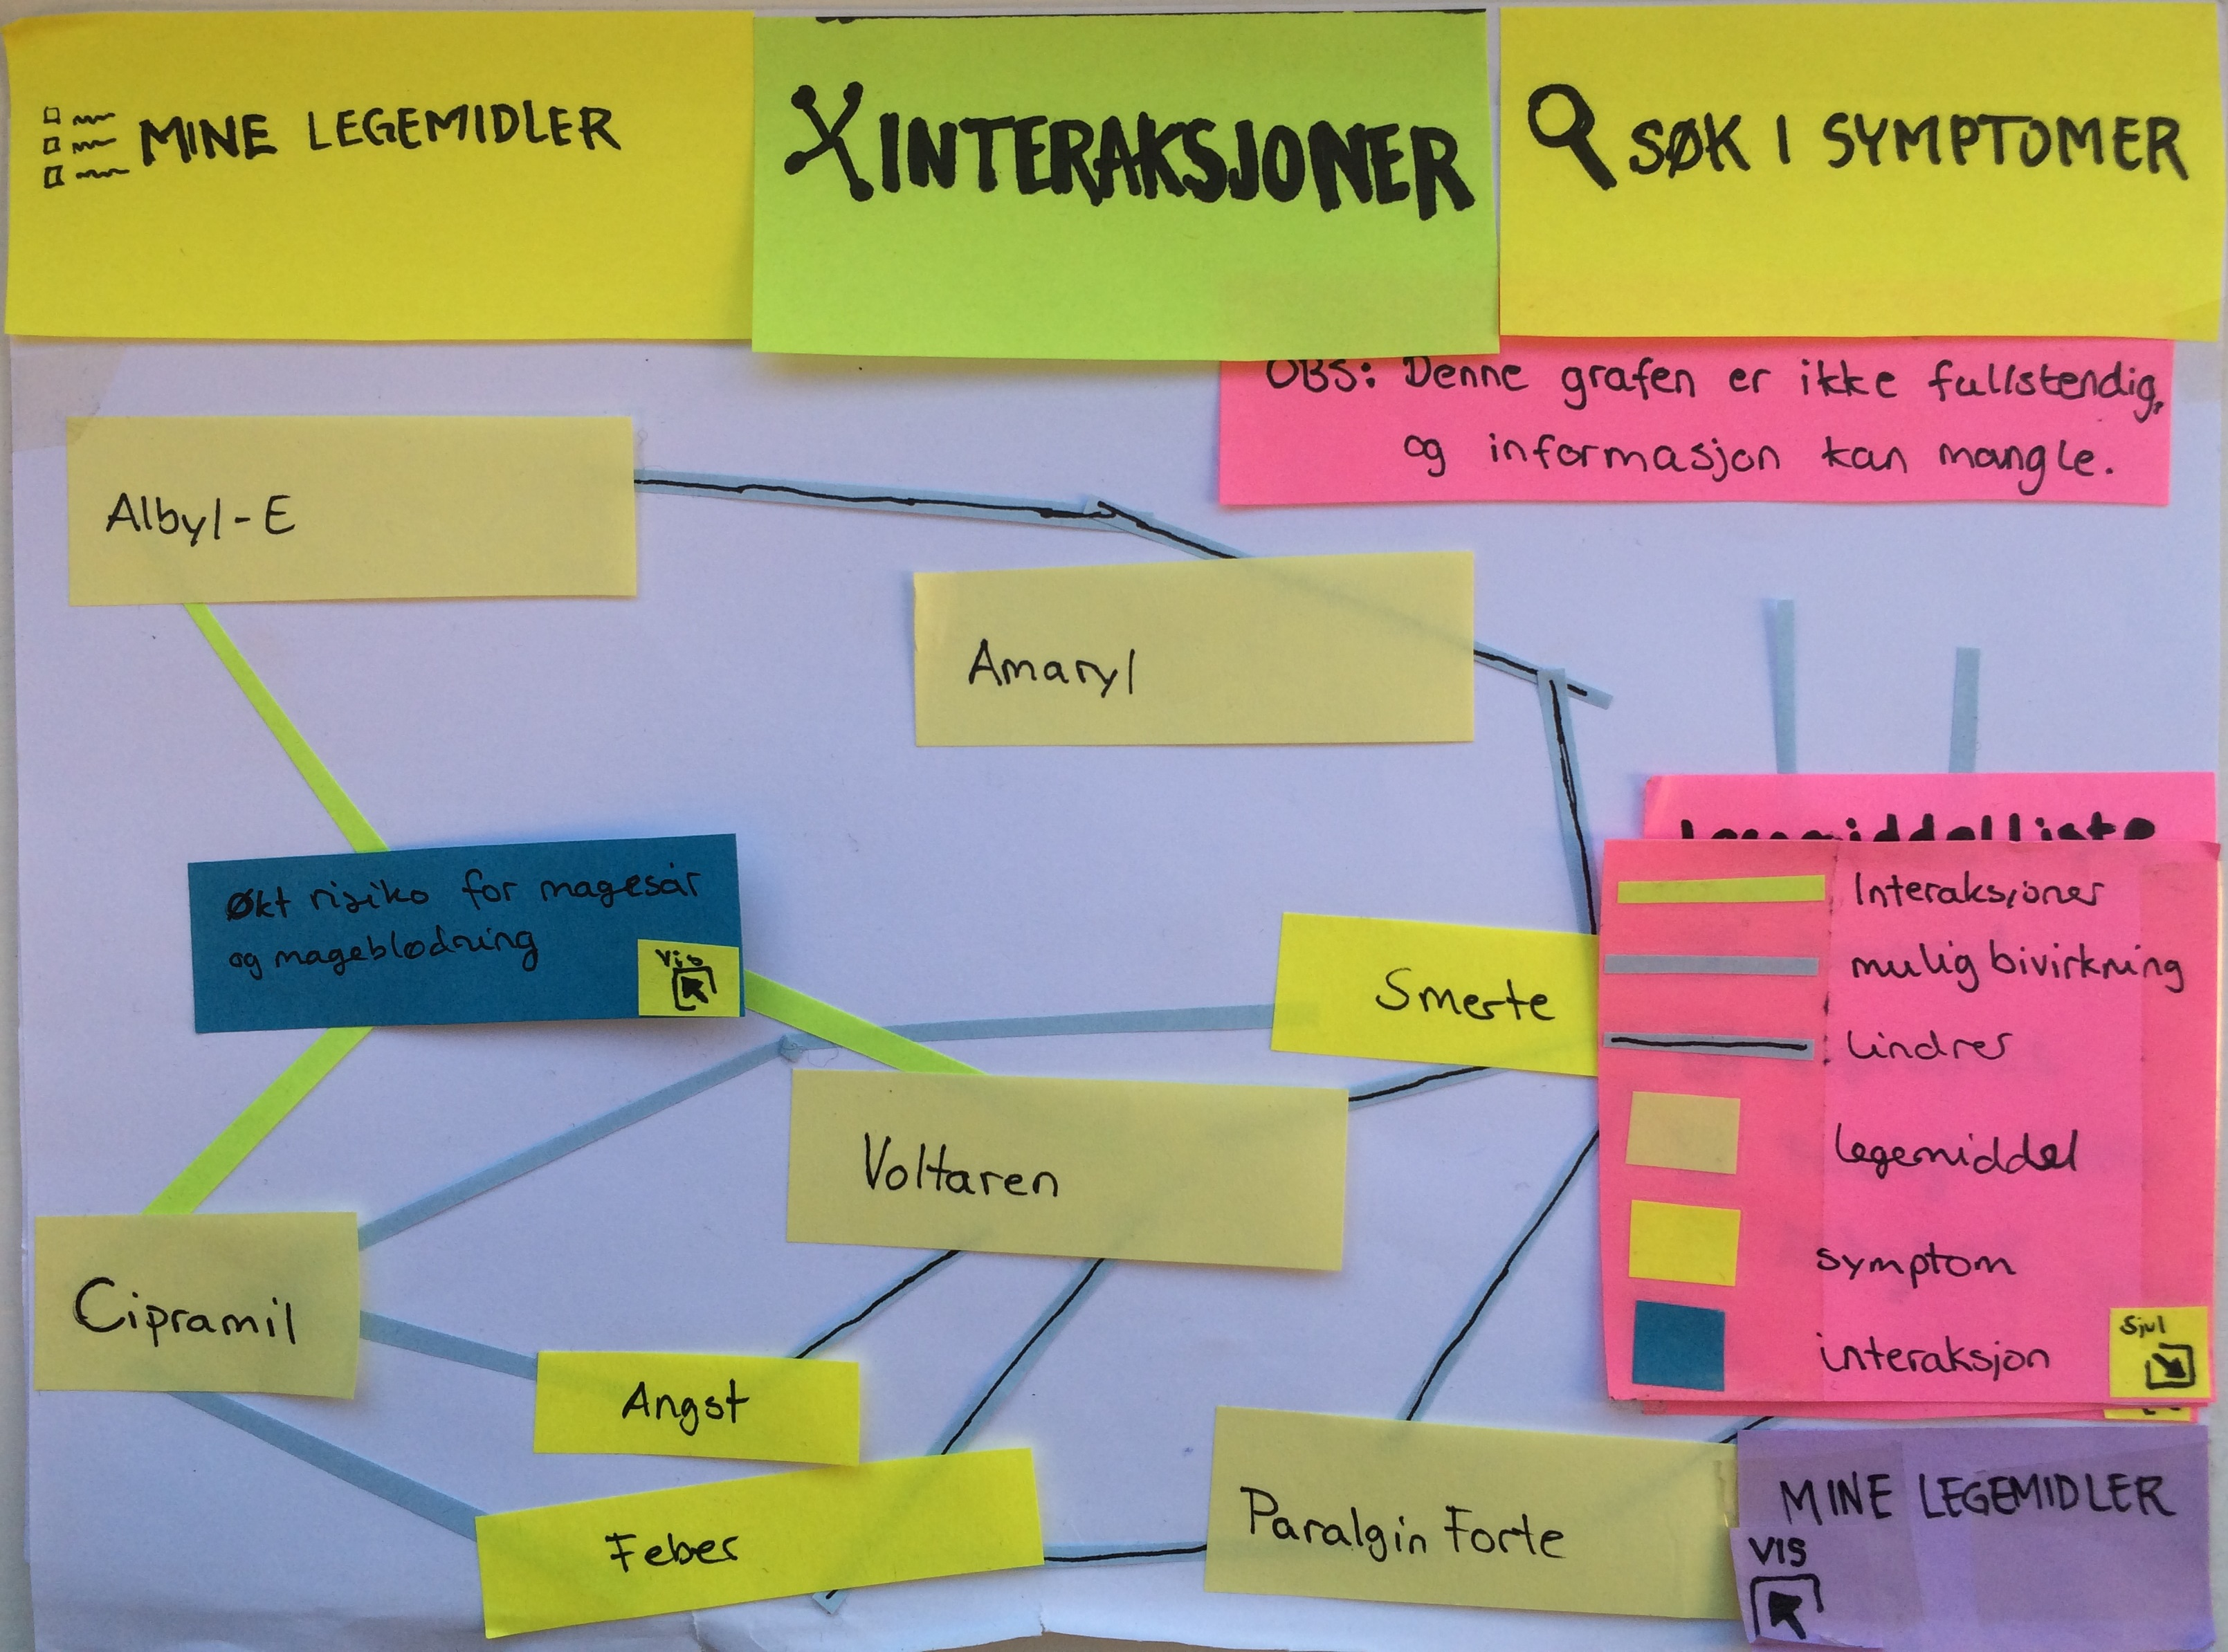
\includegraphics[width=1\textwidth]{fig/utviklingAvPrototype/interaksjonsgrafPP.jpg}
    \caption{Interaksjoner}
    \label{fig:interaksjonsgrafPP}
\end{figure} 

\subsubsection{Pop-up 1: “Symptom på interaksjon“}
Dersom en interaksjonsnode klikkes på, vil en pop-up som lister mulige symptomer på interaksjonen komme opp. En slik pop-up er vist som en grønn post-it på figur~\ref{fig:interaksjonsgrafInfoPP}.

\begin{figure}[H]
    \centering
    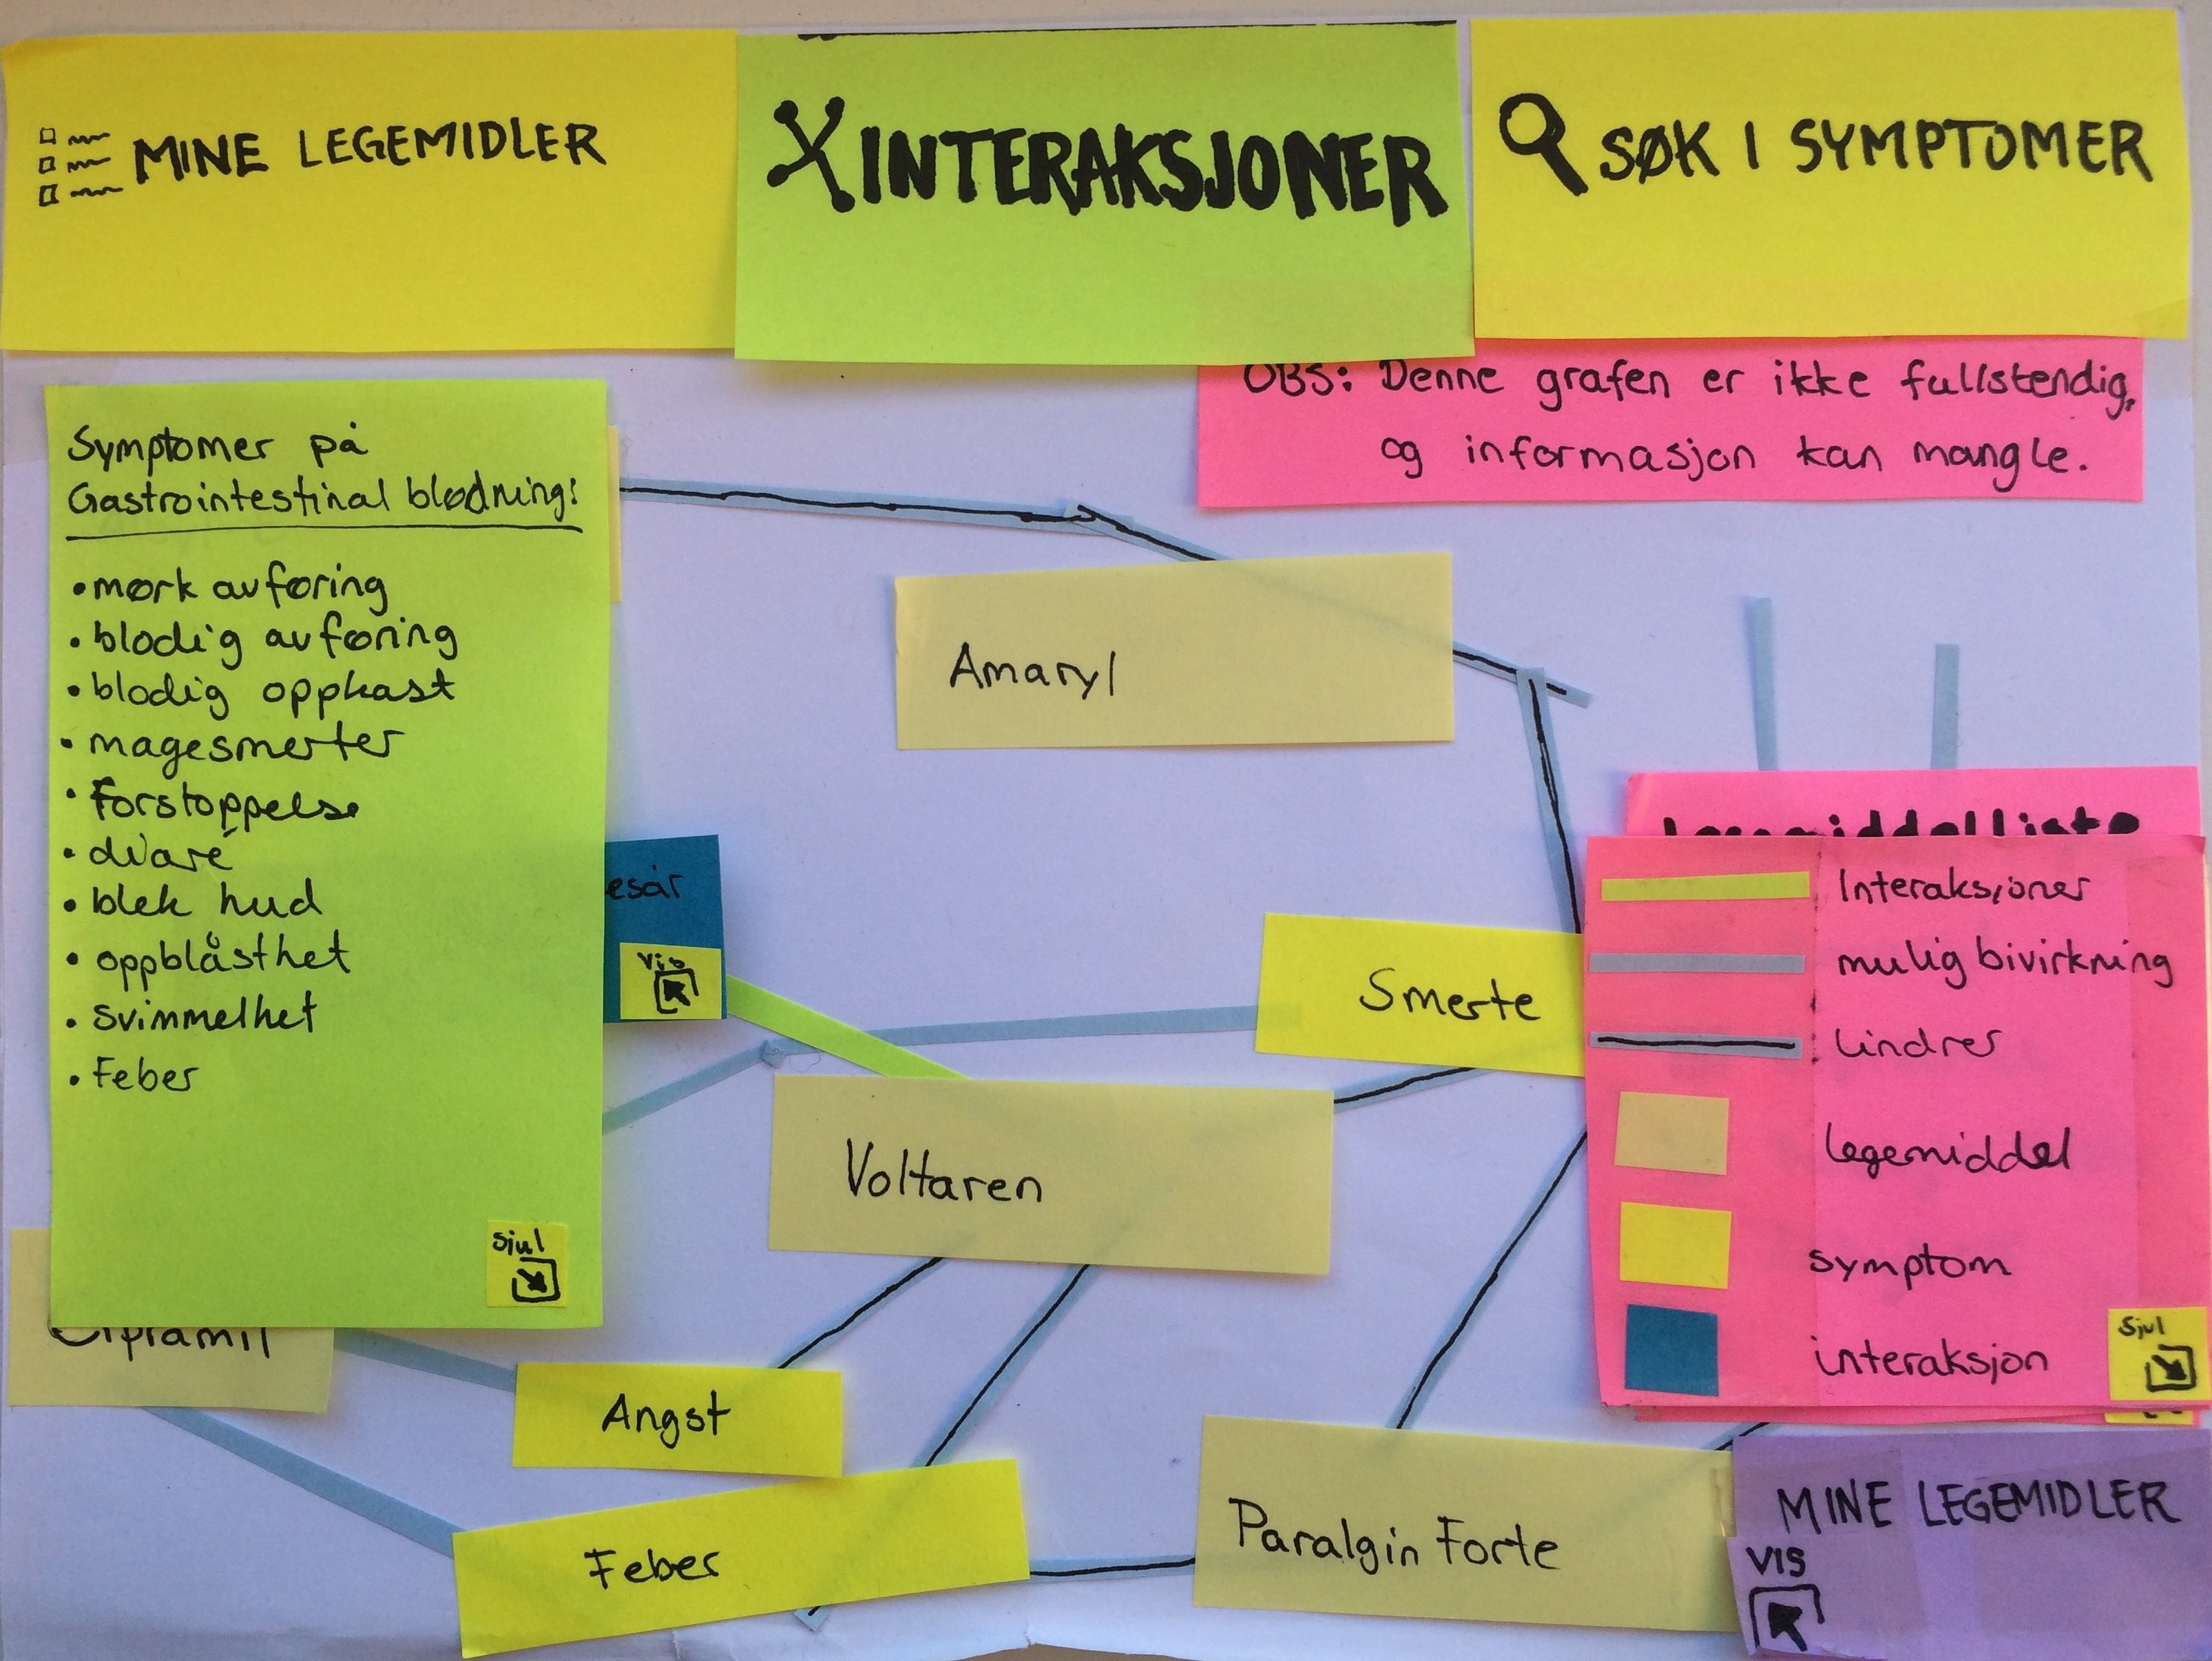
\includegraphics[width=1\textwidth]{fig/utviklingAvPrototype/interaksjonsgrafInfoPP.jpg}
    \caption{“Symptom på interaksjon” for gastrointestinal blødning som en grønn post-it}
    \label{fig:interaksjonsgrafInfoPP}
\end{figure} 

\subsubsection{Side 4: “Søk i symptomer”} 
Brukeren kan søke i symptomer ved å skrive inn fritekst, eller ved å klikke på kroppsdelen, symptomet er relatert til, på en figur. Figur~\ref{fig:sokForPP} viser hvordan “søk i symptomer”-siden til papirprototypen ser ut.

\begin{figure}[H]
    \centering
    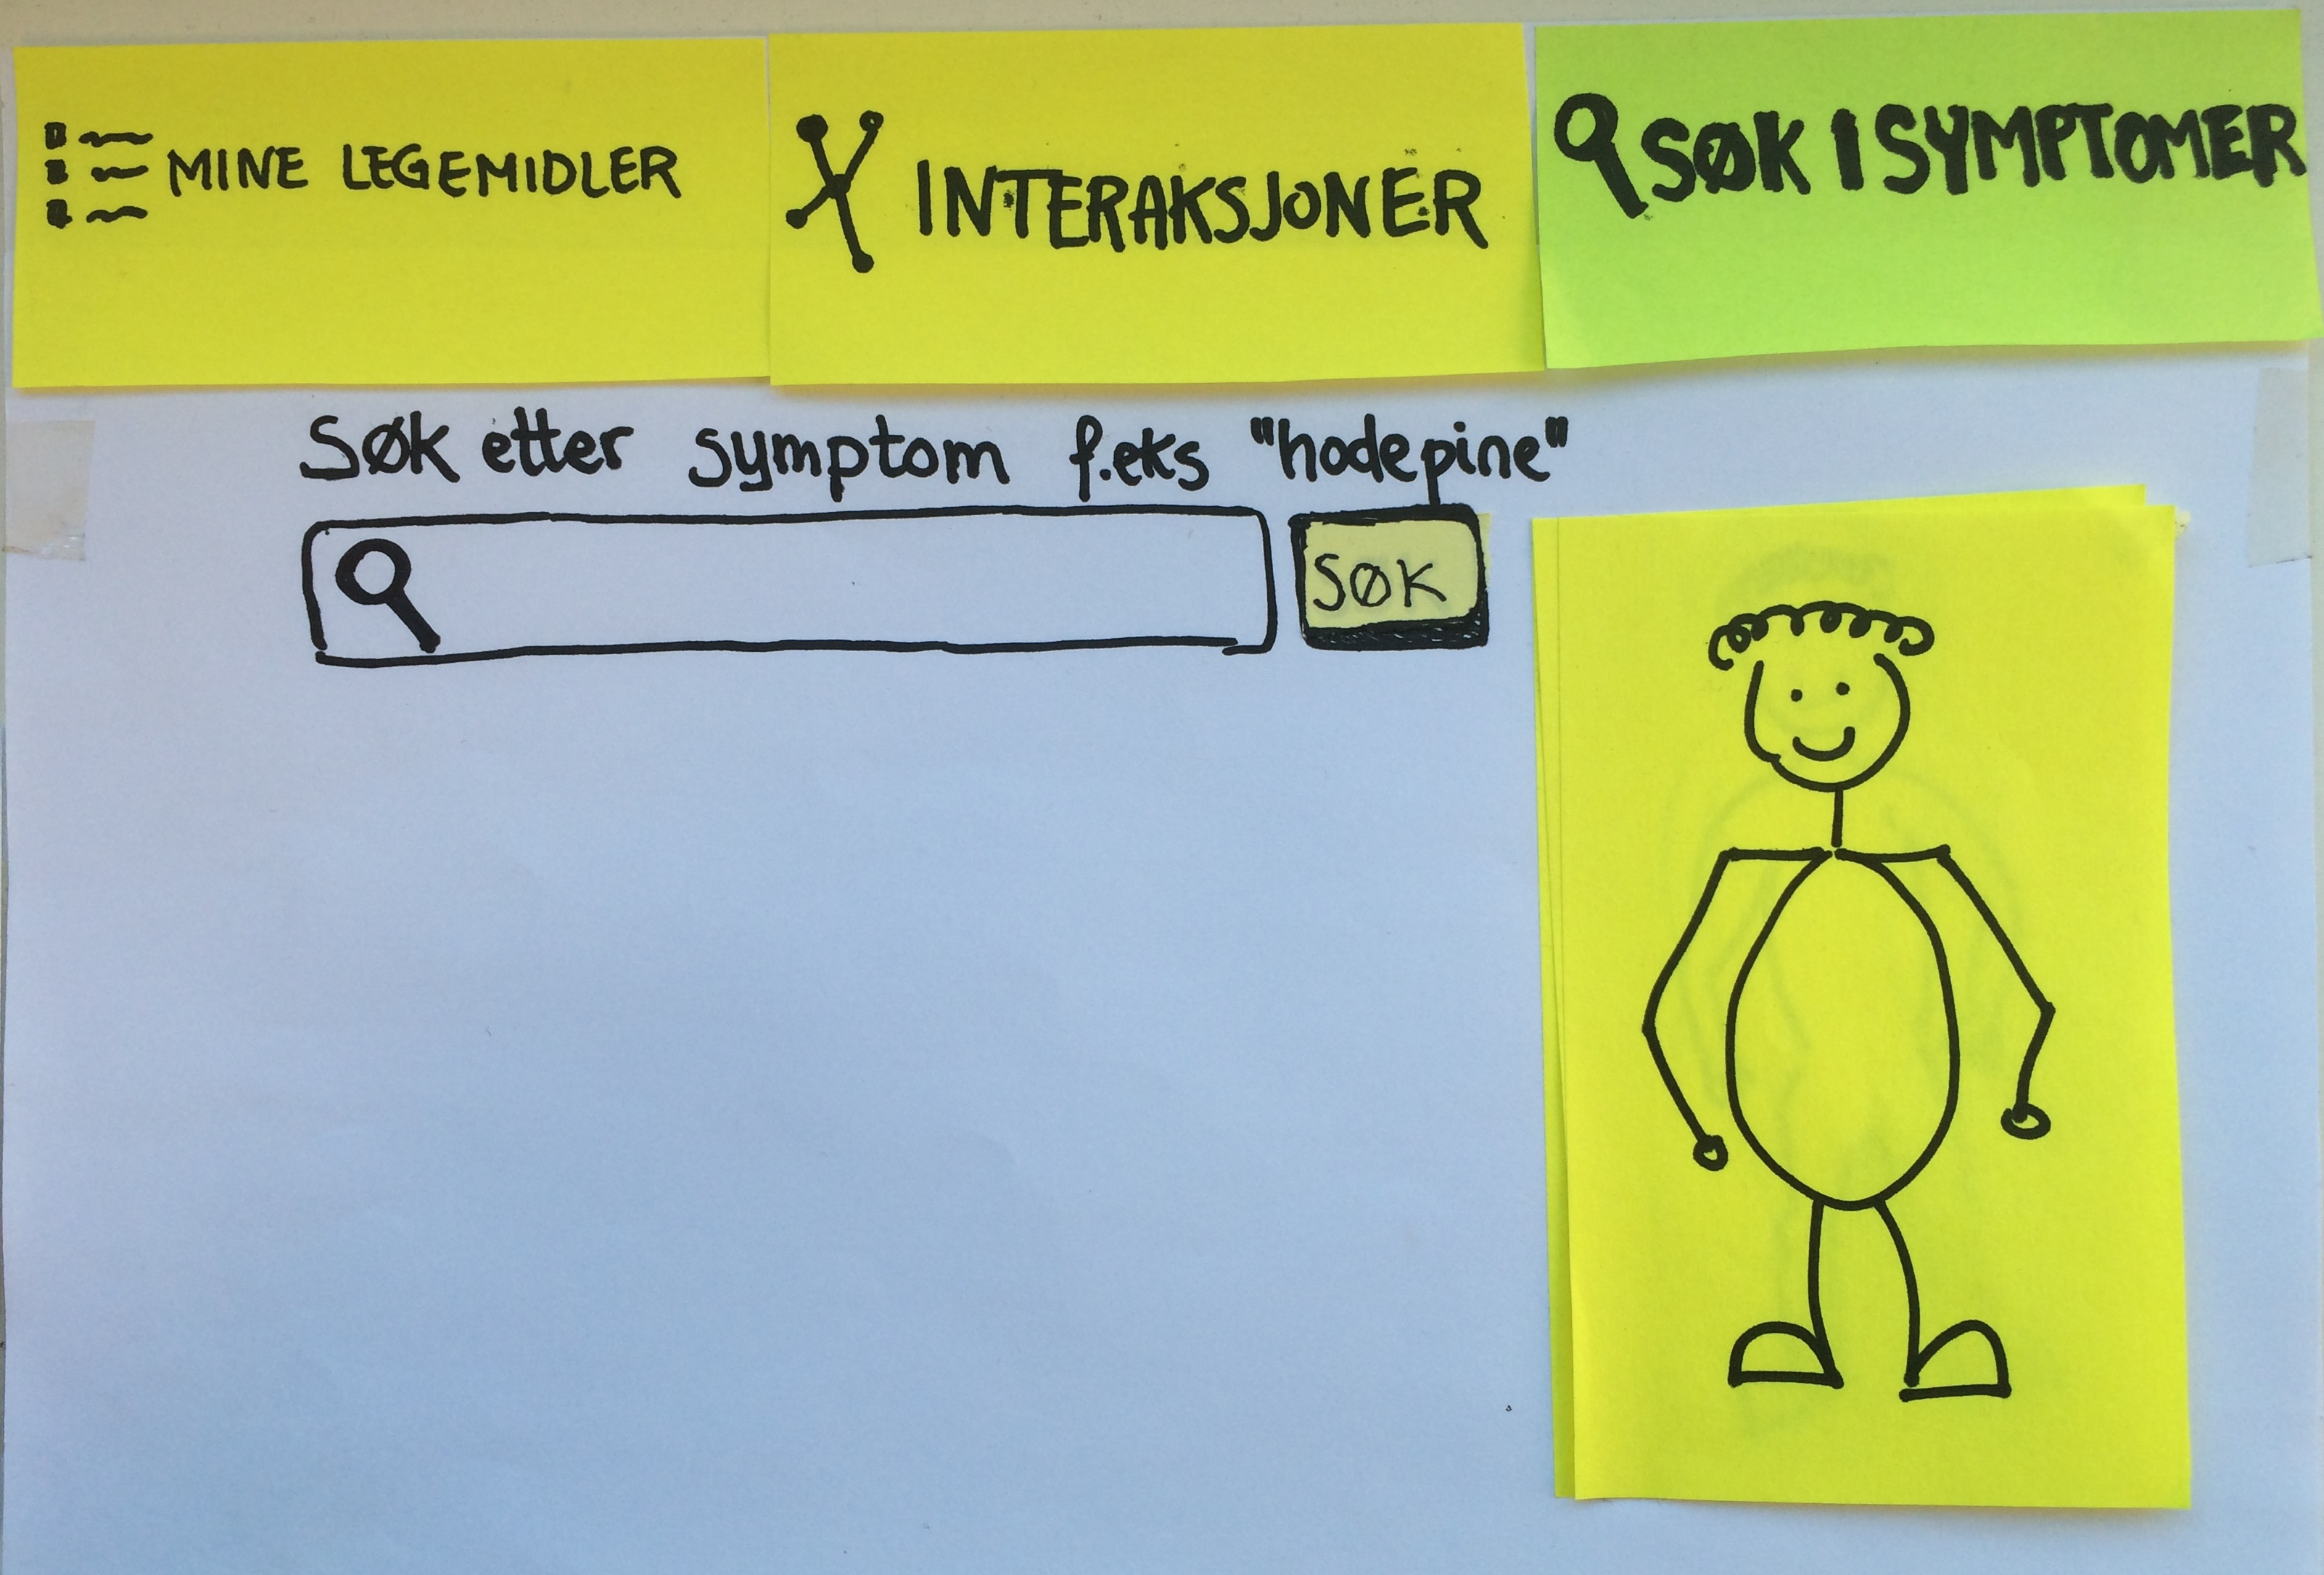
\includegraphics[width=1\textwidth]{fig/utviklingAvPrototype/sokForPP.jpg}
    \caption{“Søk i symptomer”}
    \label{fig:sokForPP}
\end{figure} 

Resultatet på et søk i symptomer viser alle mulige relasjoner mellom symptomet og legemiddelene i den personlige legemiddellisten. Symptomet kan være grunnen til at pasienten tar legemiddelet, en bivirkning eller et symptom på en interaksjon mellom en kombinasjon av legemidler i legemiddellisten. Figur~\ref{fig:sokEtterPP} viser hvordan resultatlisten, ved et søk på forstoppelse, kan se ut.

\begin{figure}[H]
    \centering
    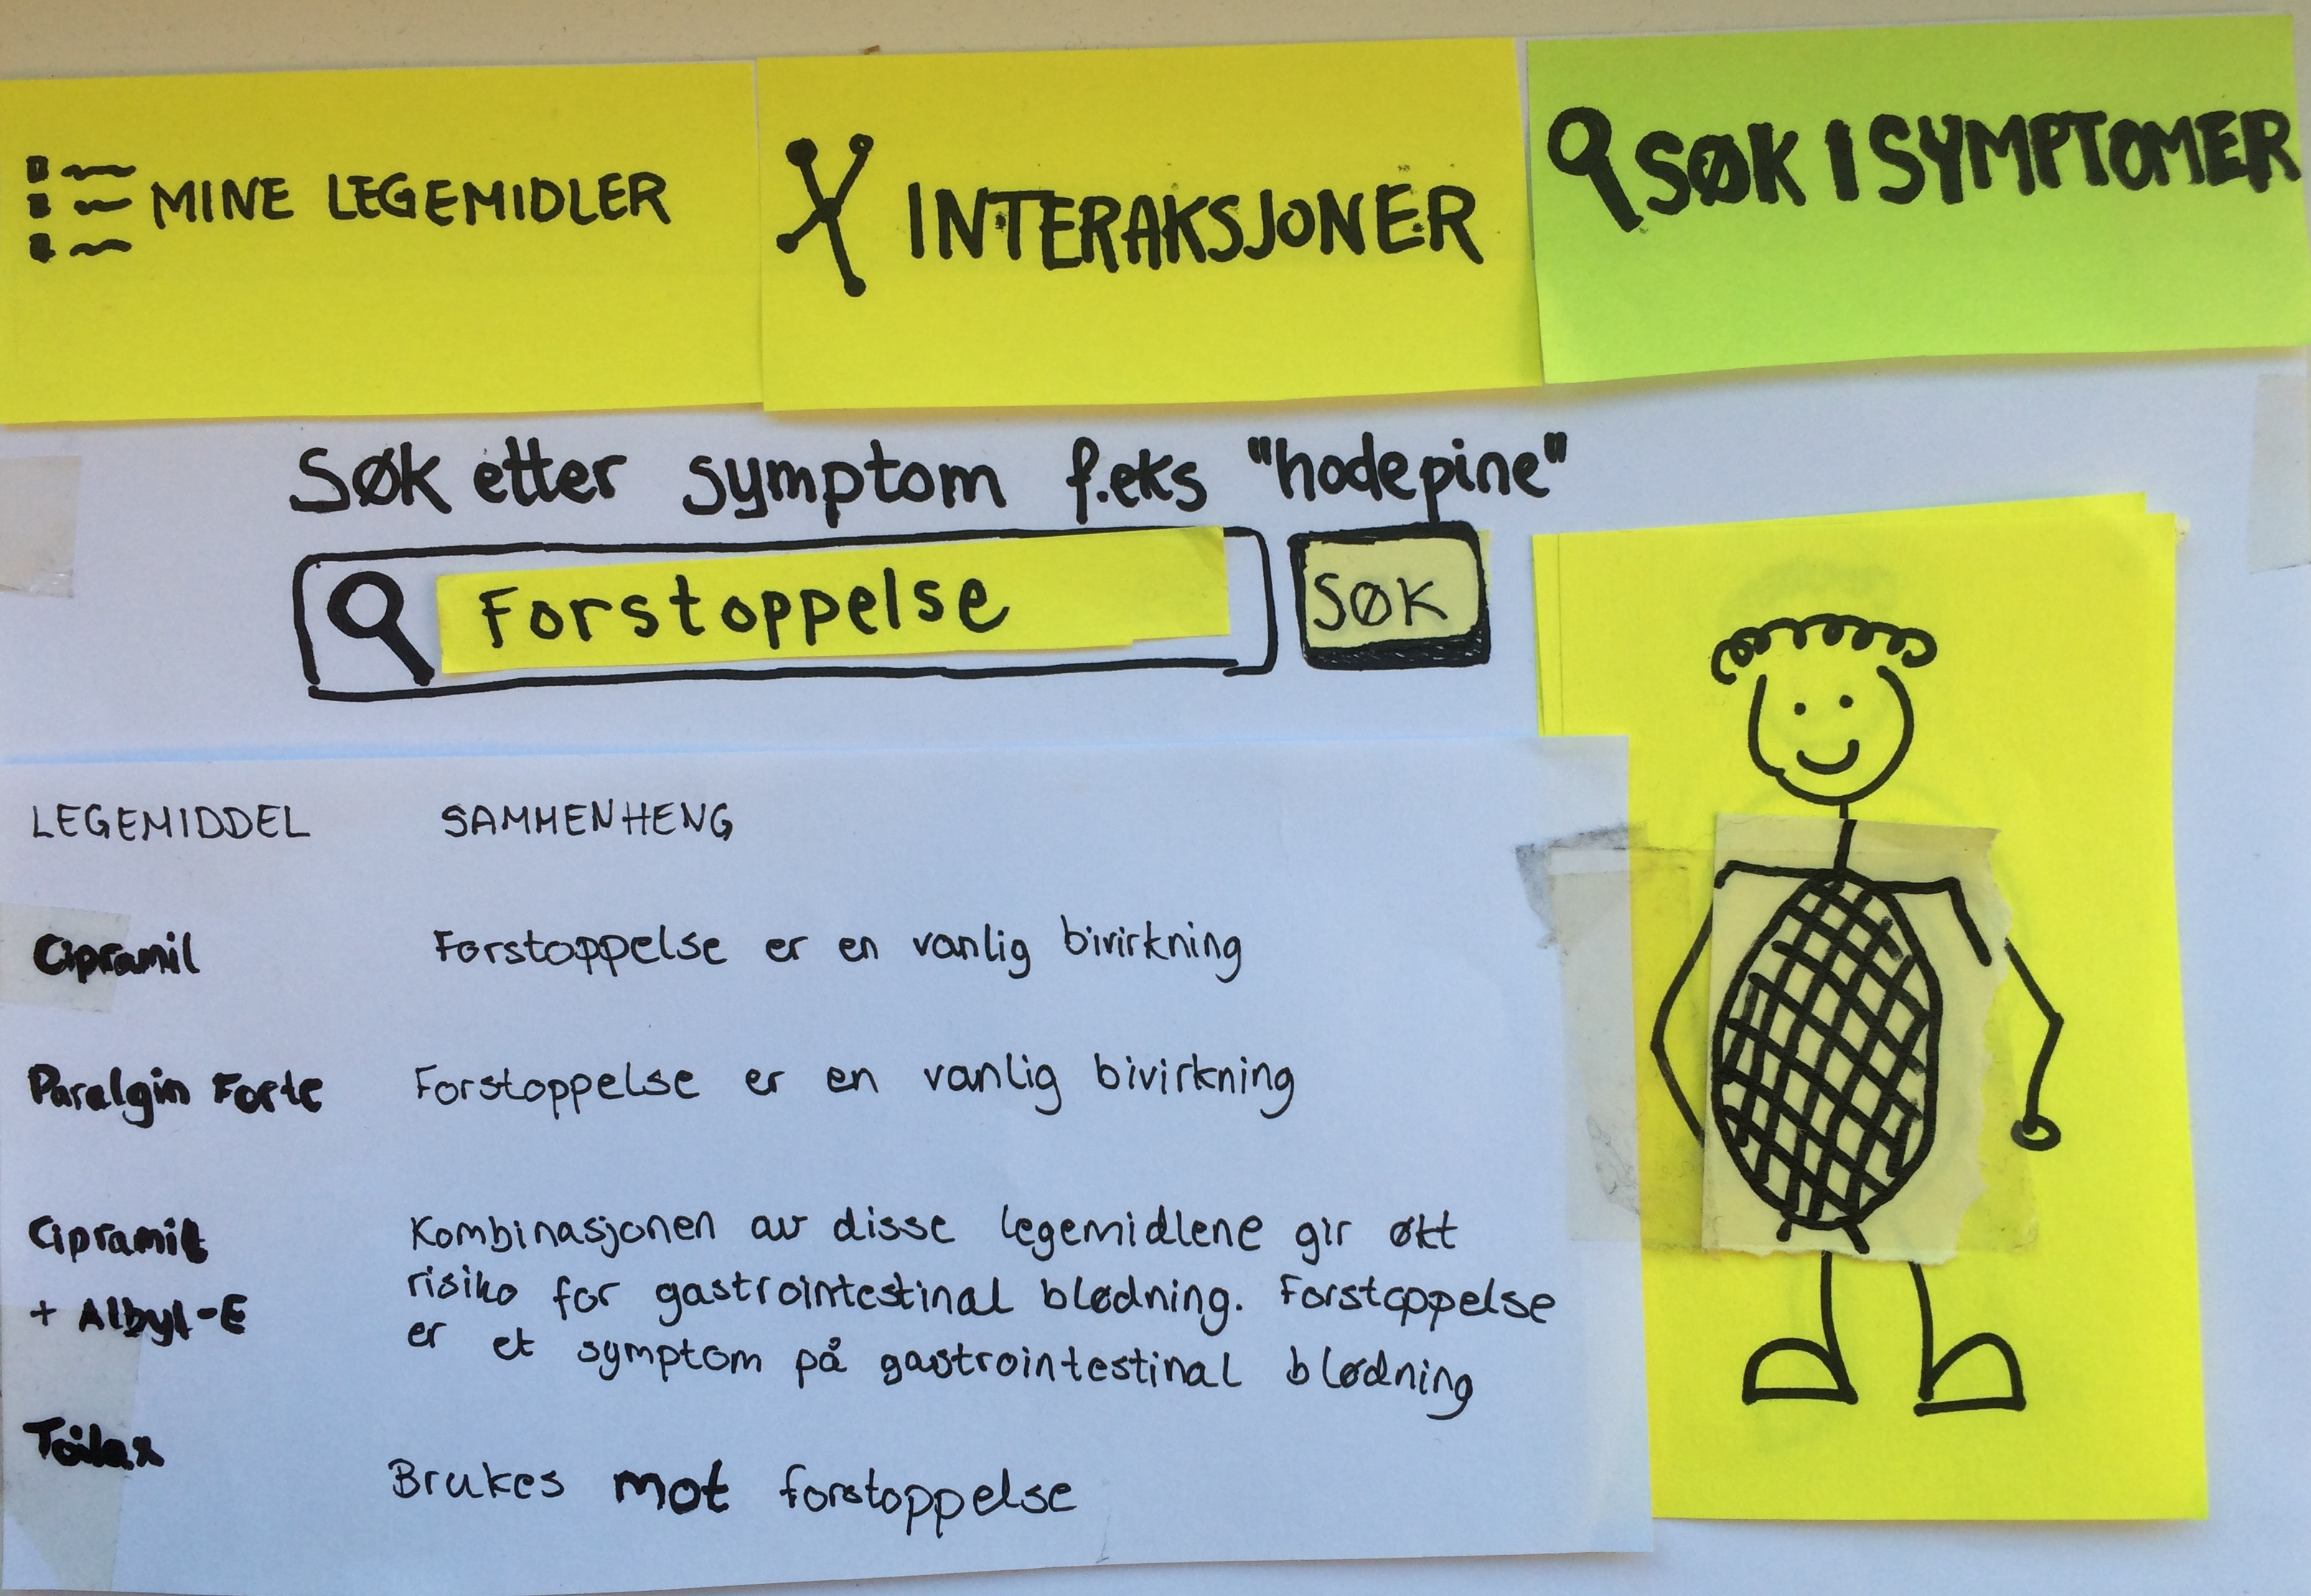
\includegraphics[width=1\textwidth]{fig/utviklingAvPrototype/sokEtterPP.jpg}
    \caption{Søk på forstoppelse}
    \label{fig:sokEtterPP}
\end{figure} 

\subsubsection{Pop-up 2: “Legemiddelvisning”}
Alle forekomster av handelsnavnet til et legemiddel linker til en visning med mer detaljert informasjon om legemiddelet. Informasjonen inkluderer hvorfor brukeren tar legemiddelet, utløpsdato, personlige notater, vanlige bivirkninger, praktisk bruk, dose og en link til pakningsvedlegg. Se figur~\ref{fig:albyl-e} for å se hvordan visningen til legemiddelet Albyl-E ser ut.

\begin{figure}[H]
    \centering
    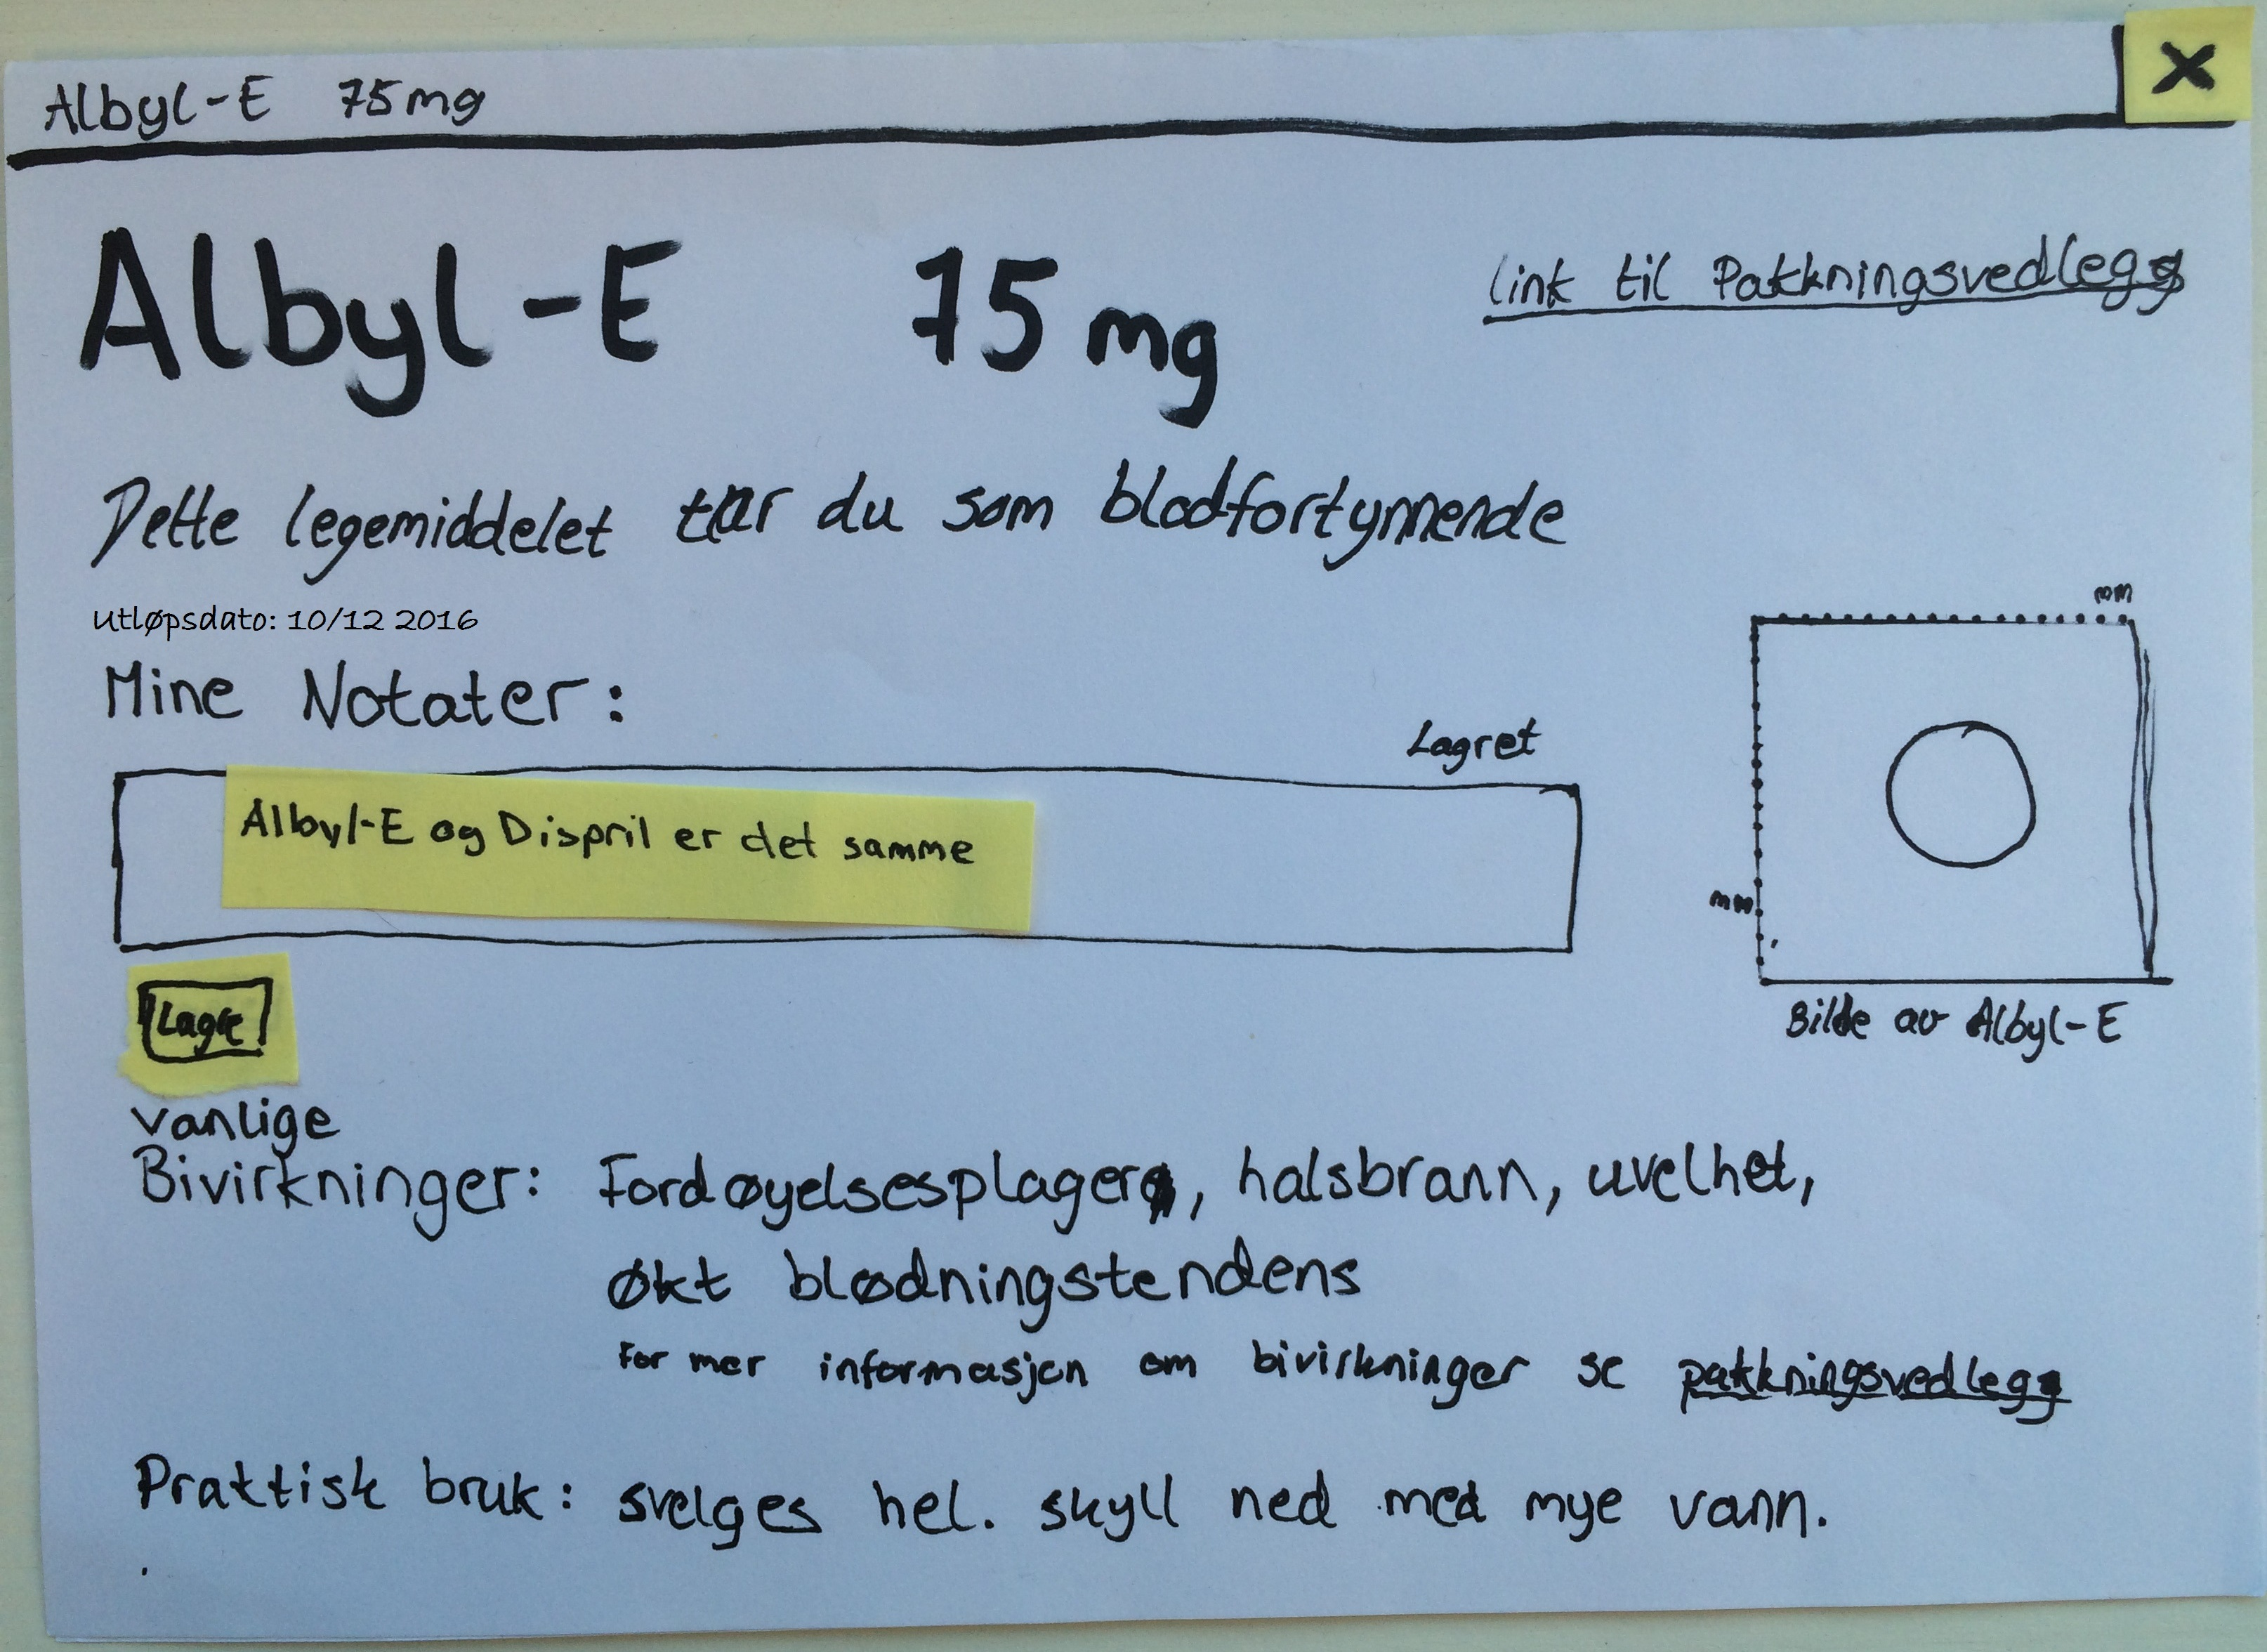
\includegraphics[width=1\textwidth]{fig/utviklingAvPrototype/Albyl-e.jpg}
    \caption{“Legemiddelvisning” for Albyl-E}
    \label{fig:albyl-e}
\end{figure} 

\section{Brukertest av første papirprototype} \label{sec:firstBrukertest}
Målet for brukertesten var å evaluere papirprototypen for å utvikle en digital prototype. For å evaluere prototypen testet vi forståeligheten av designet.

Testen ble utført på tre datateknikk-studenter, 1 kvinne og 2 menn. Å teste prototypen på deltakere som er kjent med programvareutviklingsprosessen gjorde det enkelt å forklare brukertesten og sikre at de gav relevante tilbakemeldinger. På et tidlig stadium var generelle tilbakemeldinger på forståelighet tilstrekkelig, og vi fokuserte derfor ikke på å velge deltakere fra målgruppen.

\subsection{Resultat}
Tilbakemeldinger fra brukertestene ble brukt til å identifiserte potensielle forbedringer, se tabell~\ref{tab:forbedringer}.

\begin{table}[H]
    \centering
    \begin{tabular}{|p{5cm}|p{6cm}|}
     \hline
     \textbf{Forbedringer} &         \textbf{Motivasjon} \\ \hline
     Bruke enklere språk. & Noen deltakere forsto ikke hva en interaksjon er. Det kan være fordi deltakerene ikke har kunnskap om legemidler. \\  \hline
     Gjøre det mulig å endre dose, og årsak til å ta legemiddelet i legemiddellisten. & Noen av deltakerene klikket på forskjellige steder i radene i “mine legemidler”-visningen, og forventet å få forskjellige valg avhengig av hvor på raden de klikket. Hele raden linker til den samme siden med informasjon om legemiddelet.  \\  \hline
     Legge til overskrift i hvert “view”. & Flere ganger oppsto det forvirring om hvilken side de så rett etter innlogging, selv om navnet på visningen var markert i en annen farge i toppmenyen.  \\  \hline
     Gjøre interaksjonsgrafen enklere ved kun å inkludere interaksjoner, og ikke motstridende effekter. & Det virker som om interaksjonsgrafen er vanskelig å forstå, og at forklaringene er kompliserte. Noen deltakere la ikke merke til vinduet med forklaringer. \\  \hline
     Gjøre “min legemiddelliste” mer synlig i interaksjonsvisningen. & Ingen deltakere valgte å bruke “mine legemidler”-listen i interaksjonsvinduet for å fjerne legemidler fra grafen. Dette kan være fordi de er førstegangsbrukere, og at mer erfarne brukere hadde funnet denne funksjonaliteten nyttig.  \\  \hline
     Få opp forslag indikasjonene til et legemiddel når man har lagt inn navnet på et legemiddel. Brukeren kan velge alternativer fra en dropdown meny, og er ikke tvunget til å skrive fritekst.  & Flere av deltakerene nevnte at de ikke visste hvorfor de skulle ta legemiddelet, og valgte derfor å ikke skrive inn informasjon om det.  \\  \hline
     \end{tabular}
    \caption{Tabell over potensielle forbedringer av Mine Medisiner }
    \label{tab:forbedringer}
\end{table}

\section{Digital prototype} \label{sec:digitalPrototype}
I denne delen beskrives den digitale prototypen av Mine Medisiner. 
\textbf{Prototypen er tilgjengelig på \todo{FIX link}}. 

Prototypen et utviklet med utgangspunkt i kravene i tabell~\ref{tab:krav} og~\ref{tab:forbedringer}. Den er hardkodet til å fungere for Kåre, Klara og Håkon, se vedlegg~\ref{chap:kaare}, ~\ref{chap:klara} og ~\ref{chap:haakon}. I dette delkapittelet brukes skjermbilder for Kåre sin legemiddelsituasjon til å demonstrere systemets funksjonaliteter.

\subsection{Velkommen og logg inn}
Figur~\ref{fig:velkommen} viser forsiden og figur~\ref{fig:logginn2} viser innloggingssiden til Mine Medisiner. Brukere kan logge inn i Mine Medisiner med brukernavn og passord, som vist i tabell~\ref{tab:logginn}.

\begin{table}[H]
    \centering
    \begin{tabular}{|c|c|}
     \hline
     \textbf{Brukernavn} &         \textbf{Passord} \\ \hline
     kaare & 1234 \\  \hline
     klara & 1234  \\  \hline
     haakon & 1234  \\  \hline
     \end{tabular}
    \caption{Brukernavn og passord Mine Medisiner støtter}
    \label{tab:logginn}
\end{table}

\begin{figure}[H]
    
\includegraphics[width=\textwidth]{fig/utviklingAvPrototype/velkommen.PNG}
    \caption{“Velkommen til Mine Medisiner”}\label{fig:velkommen}
  \end{figure}

\begin{figure}[H]
    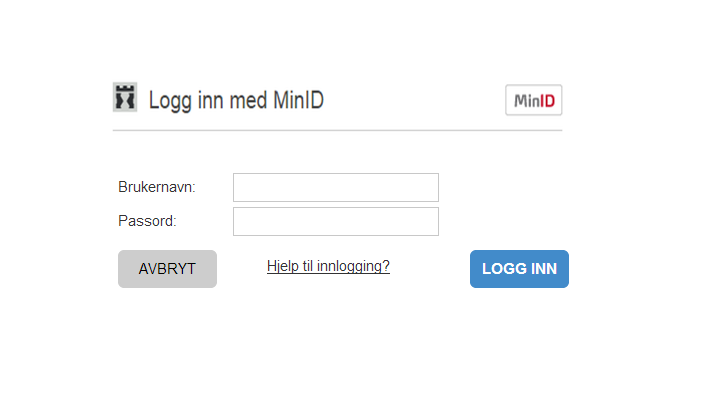
\includegraphics[width=\textwidth]{fig/utviklingAvPrototype/logginn2.PNG}
    \caption{“Logg inn med MinId”}\label{fig:logginn2}
\end{figure}

\subsection{Mine Legemidler}
Systemet består av tre faner, “Mine legemidler”, “Interaksjoner” og “Søk i symptomer”. Disse kan navigeres mellom ved hjelp av navigasjonsbaren øverst. 
Etter innlogging får brukeren opp skjermen som viser brukerens legemidler, se figur~\ref{fig:mineLegemidler}. Det er mulig å legge til og slette legemidler fra lista.

\begin{figure}[H]
    \centering
    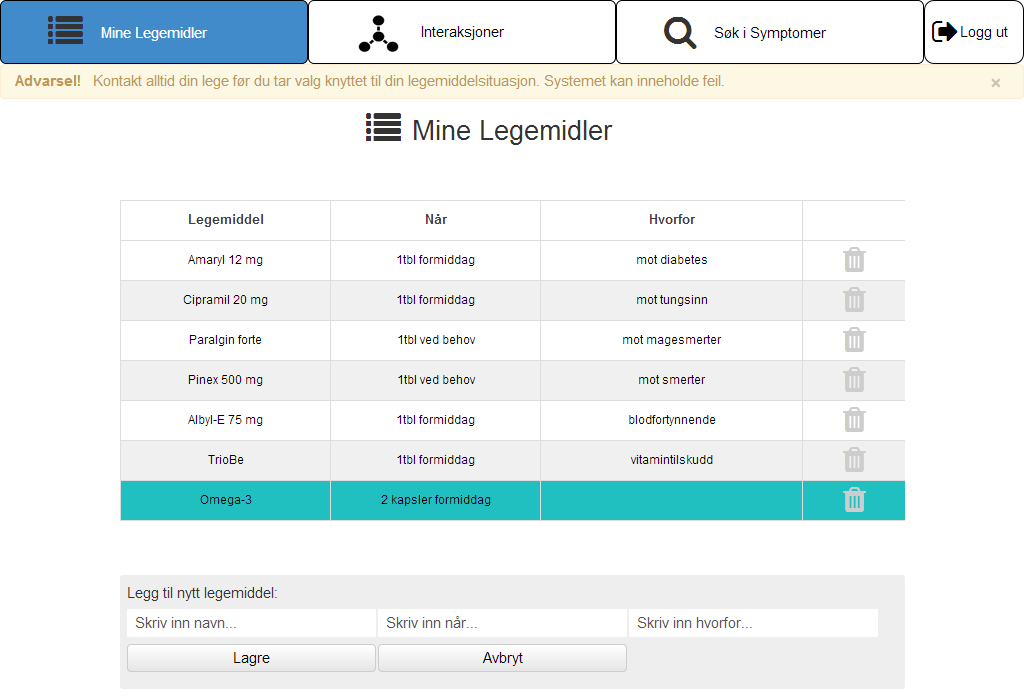
\includegraphics[width=1\textwidth]{fig/utviklingAvPrototype/mineLegemidler.PNG}
    \caption{Mine Legemidler}
    \label{fig:mineLegemidler}
\end{figure} 

\subsubsection{Legg til legemiddel}
Når brukeren skal legge inn et legemiddel vil systemet gi brukeren ulike indikasjoner knyttet til dette legemiddelet. I figur~\ref{fig:voltaren} har brukeren skrevet inn “Voltaren 50 mg”. Når brukeren så skal skrive inn hvorfor han tar Voltaren, vil det komme opp et vindu som gir mulighet til å velge den indikasjonen som stemmer, eller skrive årsak selv. De ulike  brukerene i prototypen har denne funksjonaliteten for Ibux, Voltaren og Renitec. Systemet støtter kun automatisk oppdatering av interaksjonsgrafen og søkeresultater hvis Renitec legges til i legemiddellisten til Håkon. 

\begin{figure}[H]
    \centering
    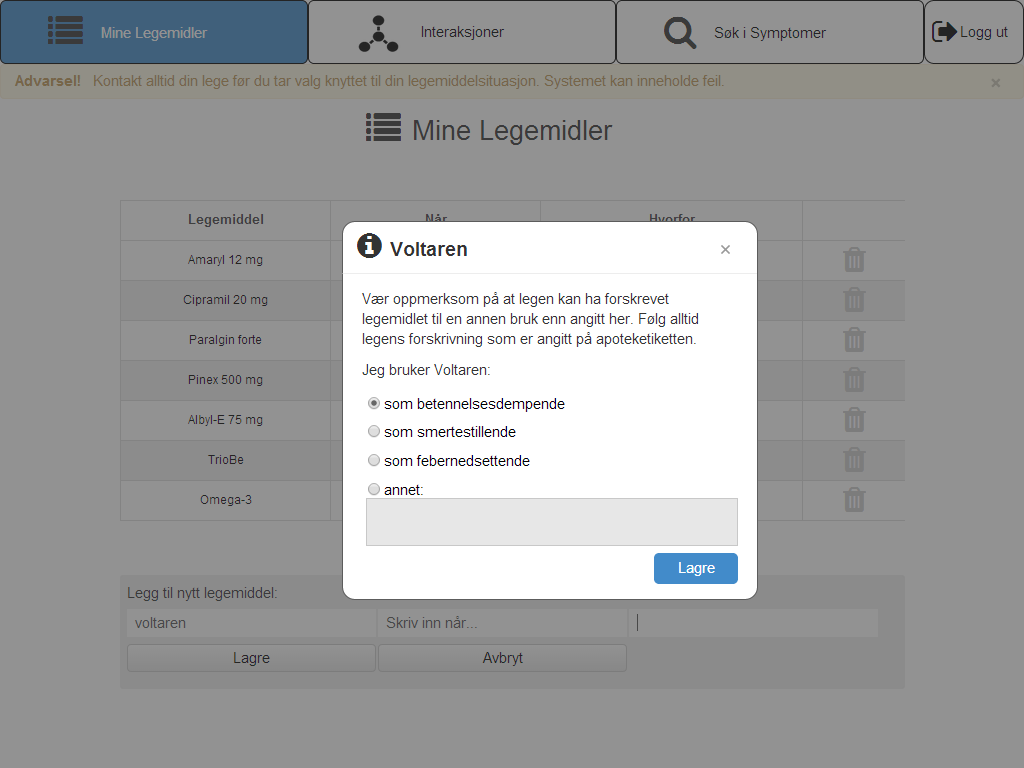
\includegraphics[width=1\textwidth]{fig/utviklingAvPrototype/Voltaren.PNG}
    \caption{Legg til Voltaren i legemiddellisten}
    \label{fig:voltaren}
\end{figure} 

\subsection{Generell legemiddelinformasjon}\label{subsec:generellInfo}
Hvis brukeren ønsker å vite mer om et enkelt legemiddel, kan han klikke på et av legemidlene i legemiddellista. Ved å trykke på “Amaryl 12 mg” i legemiddellista til Kåre vil brukeren se skjermen i figur~\ref{fig:amaryl}. Her kan brukeren finne følgende informasjon:

\begin{itemize}
\item hvorfor brukeren tar legemidlet
\item egne notater
\item bilde av legemiddelet
\item vanlige bivirkninger
\item hvordan brukeren skal ta legemiddelet
\item om brukeren kan kjøre bil eller bruke maskiner etter å ha tatt legemiddelet
\end{itemize}

\begin{figure}[H]
    \centering
    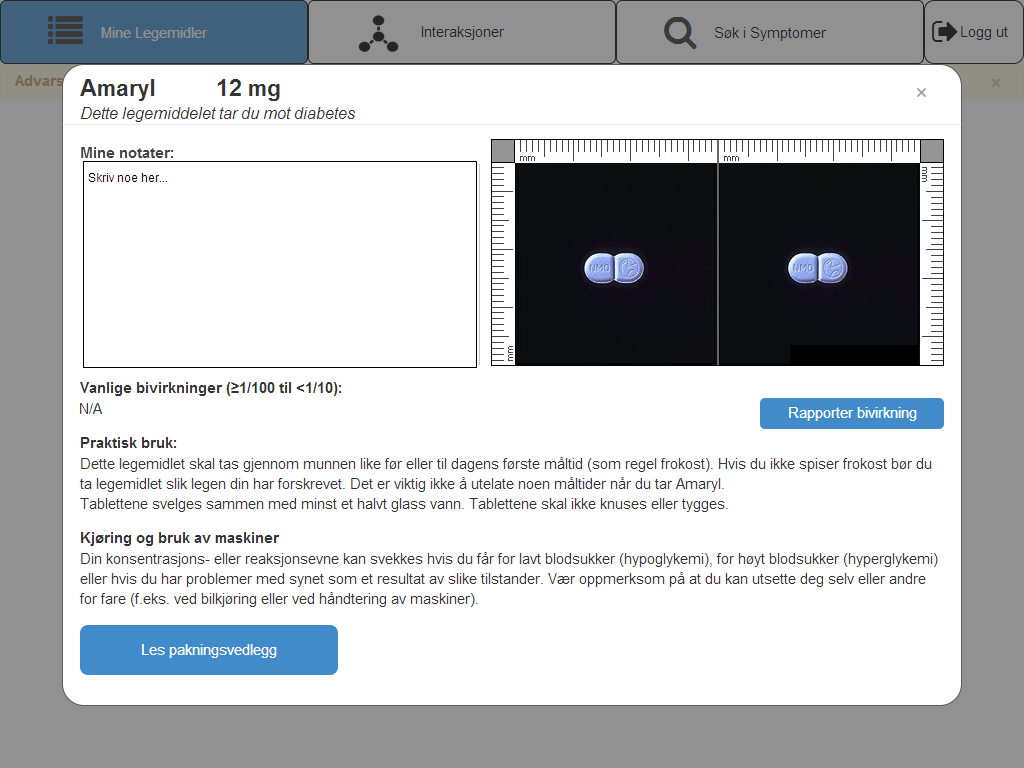
\includegraphics[width=1\textwidth]{fig/utviklingAvPrototype/amaryl.PNG}
    \caption{Generell legemiddelinformasjon om Amaryl}
    \label{fig:amaryl}
\end{figure} 

Ved å å trykke på “les pakningsvedlegg”-knappen vil det aktuelle pakningsvedlegget fra Felleskatalogen åpnes i et pop-upvindu. 

“Rapporter bivirkning”-knappen vil åpne et pop-upvindu med legemiddelverket sin “bivirkningsmeldig for pasienter”-side. Slik kan pasienten lett melde opplevde bivirkninger.

\subsection{Interaksjoner} \label{subchap:interaksjoner}
“Interaksjoner”-delen av Mine Medisiner viser brukerens legemidler og deres interaksjoner. Blå sirkler representerer legemidler, rektangler av ulik farge representerer interaksjoner og trekanter forteller brukeren at to legemidler har samme virkestoff. 

\begin{figure}[H]
    \centering
    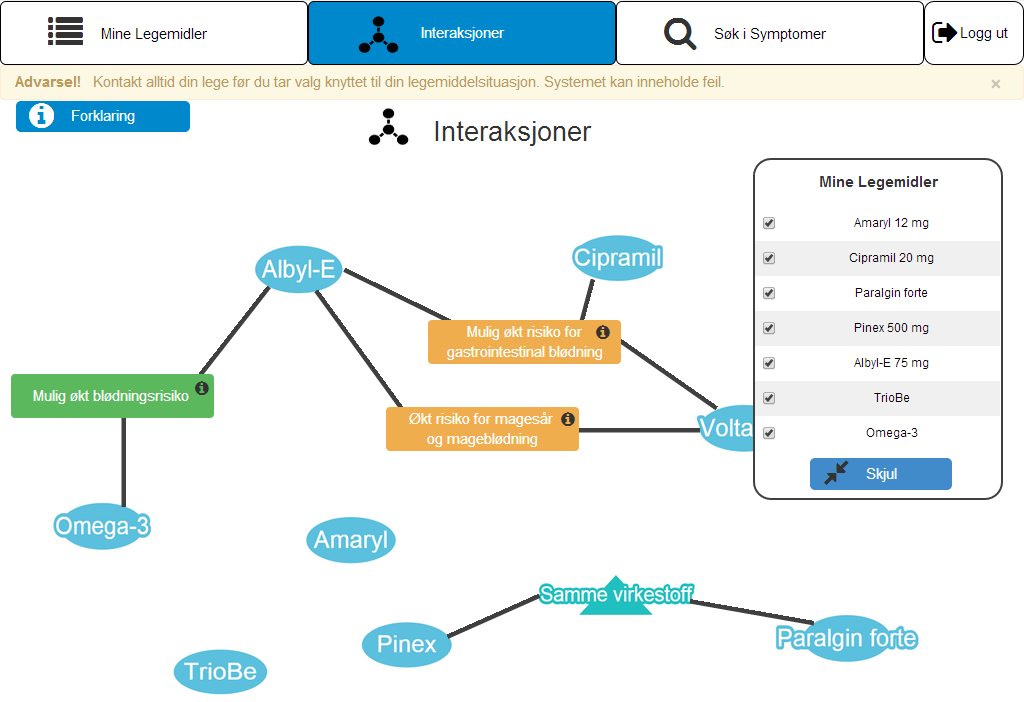
\includegraphics[width=1\textwidth]{fig/utviklingAvPrototype/interaksjonsGraf.PNG}
    \caption{Interaksjoner}
    \label{fig:interaksjonsGraf}
\end{figure} 

Rektanglene som representerer interaksjoner er fargekodet. Et rødt rektangel betyr at legemidlene ikke bør kombineres. Gule rektangler betyr at man bør ta forholdsregler når man tar den gitte kombinasjonen av legemidler. Grønne rektangler er interaksjoner av akademisk interesse. Akademisk interesse vil si at studier viser at de disse legemidlene kan kombineres, men enkeltindivider har opplevd effekter av interaksjonen. Fargekodingen og forklaringene er de samme som er brukt på \url{www.interaksjoner.no}.

På den samme siden kan brukeren benytte seg av legemiddellisten til høyre i figur~\ref{fig:interaksjonsGraf}. Denne kan flyttes rundt, og den kan minimeres ved hjelp av \textit{skjul}-knappen. Listen gir brukeren mulighet til å eksperimentere med grafen ved å velge bort legemidler. 

Sirklene og rektanglene i grafen er klikkbare. Hvis brukeren klikker på en sirkel vil brukeren få opp den generelle informasjonen om det tilhørende legemiddelet, se delkapittel~\ref{subsec:generellInfo}. Ved å trykke på et interaksjonsrektangel, vises utdypende informasjon, som vist i figur~\ref{fig:albyl-eVoltarenInteraksjon}. Hver interaksjon har et ikon som klassifiserer interaksjoner i tre farlighetsgrader: \textit{bør ikke kombineres}, \textit{ta forholdsregler} og \textit{akademisk interesse}. 

\begin{figure}[H]
    \centering
    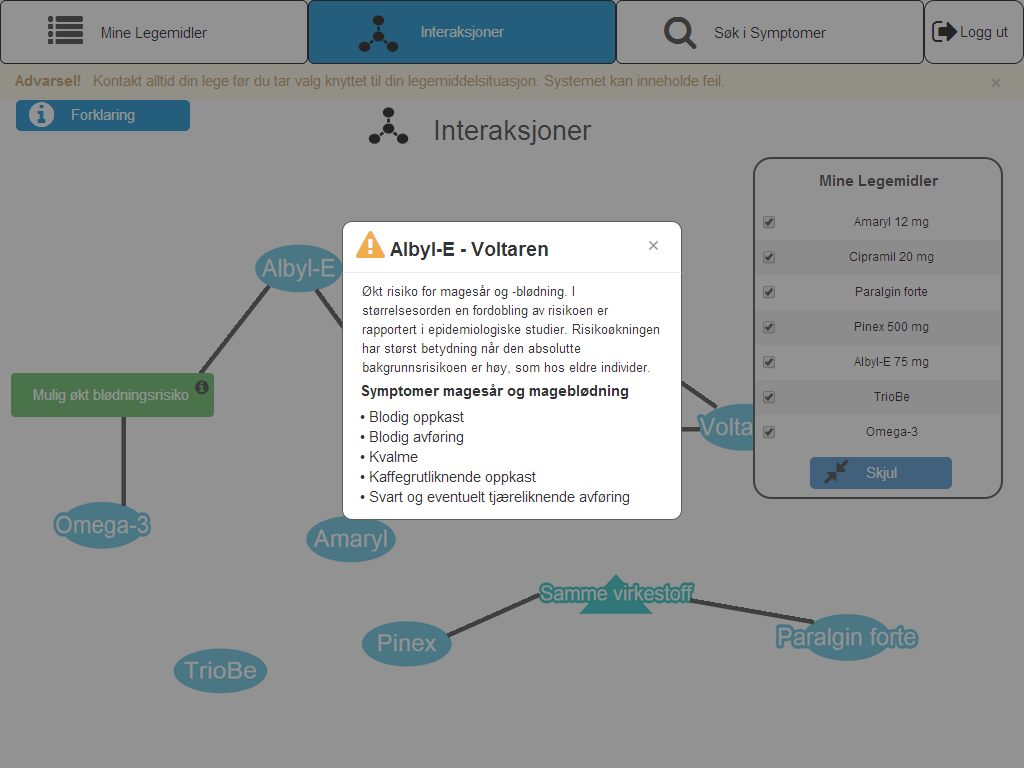
\includegraphics[width=1\textwidth]{fig/utviklingAvPrototype/albyl-eVoltarenInteraksjon.PNG}
    \caption{Albyl-E og Voltaren interaksjonsinformasjon}
    \label{fig:albyl-eVoltarenInteraksjon}
\end{figure} 


Ved å trykke på “Forklaring”-knappen vil et pop-upvindu med forklaring av interaksjonsgrafen vises, som i figur~\ref{fig:forklaring}.

\begin{figure}[H]
    \centering
    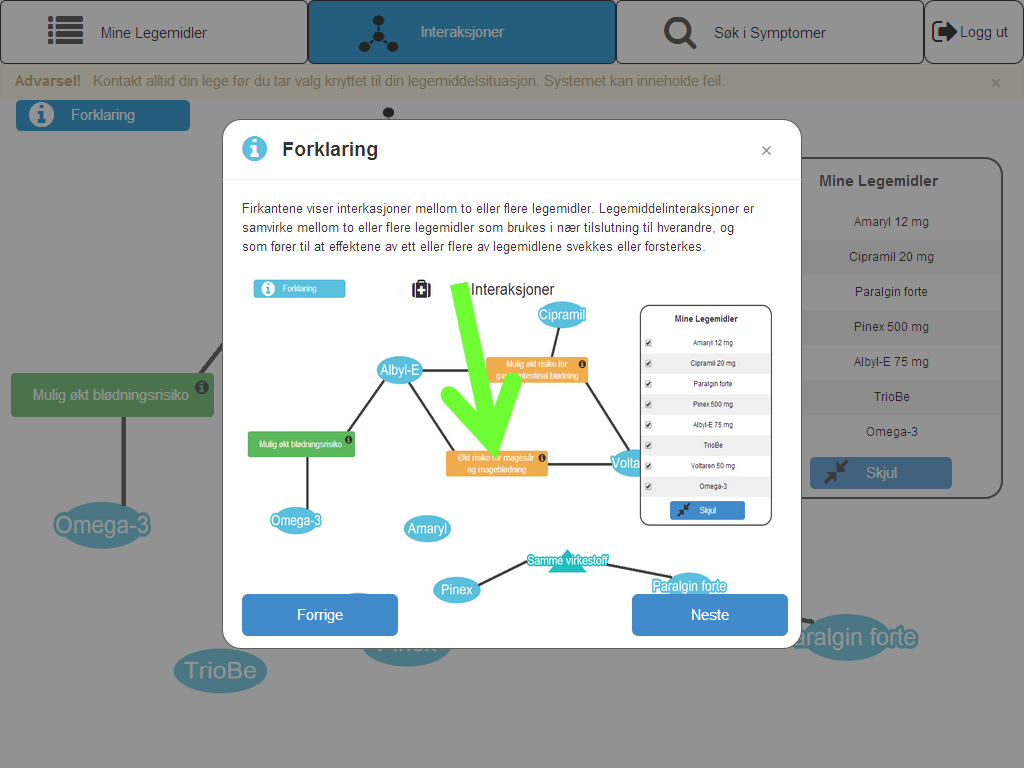
\includegraphics[width=1\textwidth]{fig/utviklingAvPrototype/Forklaring.PNG}
    \caption{Forklaring av funksjonalitet i interaksjonsfanen}
    \label{fig:forklaring}
\end{figure} 

\subsection{Søk i symptomer}
Den siste delen av systemet består av et symptomsøk, som vist i figur~\ref{fig:sokSymptomer}. 
Søkeresultatet viser legemidler i legemiddellisten som er relatert til symptomet det søkes på. Relasjonen kan være i form av en interaksjon, en bivirkninger eller en indikasjonen. Søket gir kun resultater ved søk på hodepine eller kvalme.  

\begin{figure}[H]
    \centering
    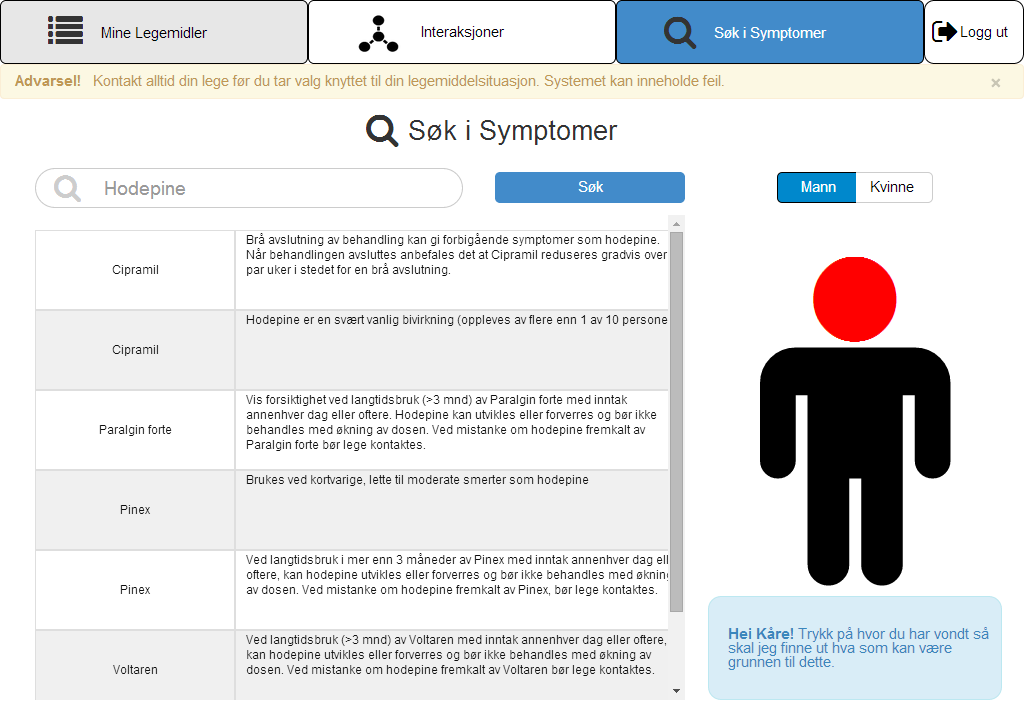
\includegraphics[width=1\textwidth]{fig/utviklingAvPrototype/sokSymptomer.PNG}
    \caption{Søk i symptomer}
    \label{fig:sokSymptomer}
\end{figure} 

Menneskefiguren til høyre i figur~\ref{fig:sokSymptomer} er klikkbar. Ved å trykke på en kroppsdel vil relevant informasjon om legemidler og symptomer vises i resultatlisten. Den klikkbare figuren støtter kun klikking på hodet.

Legemiddelnavnene i resultatlisten er klikkbare og linker til utdypende informasjon om legemiddelet, jf. delkapittel~\ref{subsec:generellInfo}, eller den tilhørende interaksjonen. 
\chapter{Gjennomføring av forsøk}\label{chap:gjennomforing}
Får å kunne svare på forskningsspørsmålet og validere hypotesene, jf. delkapittel~\ref{sec:forskningssporsmaal}, ble det gjennomført et eksperiment bestående av forsøk både på pakningsvedlegg og på Mine Medisiner. Eksperimentet fokuserte på tid, kunnskap og korrekthet. Brukbarheten til både pakningsvedlegg og Mine Medisiner ble også målt. I dette kapittelet vil utviklingen av eksperimentet, gjennomføring av forsøkene, deltakergruppen og planen for analysen av resultatene bli presentert.



\section{Utvikling av eksperimentet}
Vi bestemte oss for å gjennomføre en prøvegjennomføring av eksperimentet vi lagde. Under prøvegjennomføringen av eksperimentet fant vi noen svakheter som gjorde at vi endret eksperimentet. 

I prøvegjennomføringen hadde vi åpne spørsmål uten svaralternativer. Vi oppdaget at det var dumt at vi ikke benytte oss av svaralternativer. Ved bruk av svaralternativer ville det vært enklere å avgjøre hva som var riktige og gale svar. Dette ville gjort det lettere å sammenligne to deltakere, og å analysere resultatene. Vi fant ut at istedenfor å ha spørsmål med svaralternativer kunne det være lurt med utsagn som deltakerene vurderer hvor enig de er i. Ved å bruke en slik skala kunne vi bedre måle styrken på holdninger og opplevelser som deltakergruppen hadde. 

Prøvegjennomføringen viste at forsøket tok alt for lang tid å gjennomføre. For å korte ned tiden på forsøket gjorde vi utsagnene mer konkrete og presise. Et eksempel er at istedenfor å spørre om “Hvilke av dine legemidler har interaksjoner?” ba vi deltakerene om å vurdere utsagnet “Jeg bør ikke ta Albyl-E og Ibux.”. Dette gjorde at deltakerene ikke trengte å sjekke alle legemidlene.

En annen god effekt ved å spørre mer konkrete og presise utsagn var at pasienter som leser pakningsvedlegg eller andre kilder antagelig oftere leter etter informasjon som kan gi besvare konkrete spørsmål enn generell informasjon. Vi anså derfor det som bedre at deltakerene skal vurdere utsagnet “Jeg har hodepine fordi jeg har tatt Albyl-E.” enn at de skulle svare på “Hvilke av dine legemidler kan gi hodepine?”.

I spørsmålene i prøvegjennomføringen brukte vi ordet \textit{interaksjon}. Vi oppdaget at deltakerne ikke forstod dette ordet. Utsagnene vi formulerte til de ordentlige forsøkene inneholder derfor ikke ordet \textit{interaksjon}, men heller en lenger forklaring av hva en interaksjon er. 

Under prøvegjennomføringen valgte vi å la den samme deltakeren utføre de samme oppgavene både på pakningsvedlegg og Mine Medisiner. Årsaken til dette var fordi vi mente at det ville gjøre det enklere å sammenligne systemene. Vi oppdaget at deltakerene benyttet seg av svarene de fant ved å bruke det første systemet når de skulle finne svarene med det andre systemet. Dette gjorde det vanskeligerer å sammenligne systemene, og vi bestemte oss derfor for å at utsagnene skulel vurderes ved hjelp av et system per deltaker. Ved at deltakeren kun benytter seg av et system i et forsøk vil forsøket gå raskere, noe som var ønskelig. 

\section{Rekruttering av deltakere}
Vi ønsket å rekrutere mellom 10 og 15 \acrshort{tia}\footnote{TIA: hjerneslag hvor symptomene trekker seg tilbake i løpet av 24 timer}-pasiener til forsøkene våre. Vi tok kontakt med flere ansatte ved St. Olav universitetssykehus for å få hjelp til å rekrutere \acrshort{tia}-pasiener til forsøkene. Vi tok kontakt med både farmasøyter ansatt på sykehusapoteket og leger ansatt ved slagavdelingen. Etter flere uker med frem og tilbake måtte vi innse at det var for tidkrevende å skulle rekrutere 10-15 deltakere som har hatt \acrshort{tia}. Det var også for vanskelig å rekrutere andre pasientgrupper fra sykehuset. Vi valgte derfor å rekrutere deltakere gjennom vårt sosiale nettverk. Dette gjorde at demografien til deltakergruppen ble ganske annerledes fra det vi så for oss i utgangspunktet. 

Deltakerene ble valgt ut tilfeldig blant bekjente som hadde tid og anledning til å delta, og besto totalt av 13 personer. 6 deltakere utførte forsøk på Mine Medisiner og 7 deltakere utførte forsøk på pakningsvedlegg.
    
\section{Oppbygging av forsøket}
Forsøket besto av syv deler, se vedlegg~\ref{chap:utforming}.

Den første delen av forsøket var en introduksjon hvor deltakere ble informert om forsøket formål og utforming. deltakerene gav skriftlig samtykke til å delta i forsøket ved å signere samtykkeskjema, se vedlegg~\ref{chap:samtykke}. Skjemaet informerte om at indirekte personopplysninger vil bli slettet eller endret slik at de ikke er personidentifiserende, etter prosjektets slutt. Detaljer fra gjennomføringen av hver enkelt forsøk er ikke gjengitt i rapporten.

I forsøkets andre del ble demografiske opplysninger om deltakerne samlet inn ved at deltakeren svarte på et skjema med spørsmål om alder, yrke, utdanning, datakunnskap og legemiddelbruk, se vedlegg~\ref{chap:demografi}. De demografiske opplysningene ble samlet for å kunne bli brukt til å analysere resultatene.

Den tredje delen av forsøket besto av spørsmål om deltakeres forkunnskap om legemidler. 

Den fjerde delen, hoveddelen av forsøket, besto av syv utsagn deltakere skulle ta stilling til, se vedlegg~\ref{chap:paastander}. Utsagnene \todo{presenter utsagnenes innhold}. 
Utsagnene skulle vurderes ved hjelp av Mine Medisiner eller pakningsvedlegg. Deltakerne fikk utdelt en tekstlig beskrivelse av Håkon, se vedlegg~\ref{chap:haakon}, og ble bedt om å ta stilling til utsagnene som om de var Håkon. Den totale tiden det tok å ta stilling til de syv utsagnene ble målt for hvert forsøk. Etter at alle utsagnene var vurdert ble deltakerne bedt om å forklare årsakene til at de vurderte utsagnene som de gjorde. Ved å vente med å be om forklaringene til etter alle utsagnene var vurdert forstyrret vi deltakerene i minst mulig grad mens de vurderte utsagnene.

Den femte delen av forsøket besto av en rekke spørsmål for å sjekke om deltakeren lærte noe ved å bruke systemet, se vedlegg~\ref{chap:utforming}. Spørsmålene skulle besvares uten hjelpemidler. Noen av spørsmålene var relatert til utsagnene i del tre. Andre spørsmål var ikke eksplisitt knyttet til utsagnene, men kun til legemiddellisten generelt. Hensikten var å finne ut hvor mye deltakeren husket fra det de ble spurt om i del tre, og å finne ut hvor mye deltakerene lærte utover det som eksplisitt ble spurt om i del tre. 

I den sjette delen av forsøket fylte deltakeren ut et \acrshort{sus}-skjema for systemet de benyttet seg av under forsøket. Spørsmål 4 fra det originale \acrshort{sus}-skjemaet var endret til: “jeg vil måtte trenge hjelp fra en person med faglig kunnskap for å kunne bruke systemet”, fordi teknisk kunnskap ikke er relevant for pakningsvedlegg. Vår tolkning er at faglig kunnskap kan bety helsepersonell og teknisk personell for Mine Medisiner, og kun helsepersonell for pakningsvedlegg. Se vedlegg~\ref{chap:SUSPak} for \acrshort{sus}-skjema for pakningsvedlegg, og vedlegg~\ref{chap:SUSMM} for \acrshort{sus}-skjema for Mine medisiner.

I den syvende delen av forsøket skulle deltakeren velge 5 av 39 ord som de mente best beskrev systemet de benyttet seg av under forsøket, se tabell~\ref{tab:reactionCardTabVedlegg} i vedlegg~\ref{chap:utforming}. Etterpå skulle de begrunne valget av ord.


\section{Analyse}
Analysen av resultatene vil ta utgangspunkt i hypotesene fra delkapittel~\ref{sec:forskningssporsmaal}. Hoveddelen av analysen vil derfor gå ut på å sammenligne de to systemene. Det er vanskelig å forutse resultatene fra forsøkene. Vi antar derfor at deler av analysen ikke kan planlegges. Under presenteres den planlagte analysen, med forbehold om at resultatene vi finner ved analysen vil gi oss resultater vi kan jobbe videre med.  

\subsection{Demografi}
Demografien for forsøkene vil bli sammenlignet for å se om deltakergruppene er like. Hvis deltakergruppene er for ulike vil det være vanskelig å si noe om sammenligningsgrunnlaget for resten av observasjonene. Demografien vil også bli brukt til å prøve å validere resultatene. 

\subsection{Vurdering av utsagn}
Utsagnene har en fasit. Fasiten er utarbeidet basert på informasjon vi har funnet i pakningsvedlegg og etter samtale med farmasøyt. Vurderingsvalget og forklaringen deltakerne gir på utsagnene vil være det som vurderes mot fasiten. Altså kan det skje at``litt enig'' og en god forklaring også gir et blir godkjent som riktig, selv om vi fasiten er at ``enig'' er det riktige valget.

Tiden som ble målt når deltakerne vurderte utsagnene vil bli brukt til å si noe om hvilket system som er raskest å bruke. De demografiske forskjellene på deltakerene må tas høyde for når tidsbruken blir vurdert. 

Å tenke høyt er en mye brukt teknikk under brukertesting. Vi valgte å ikke be deltakeren tenkte høyt, da teorien var at dette ville påvirke tidtakingen. I stedet observerte vi hva deltakeren gjorde underveis, og ba om forklaring i etterkant. Forklaringen bar noen ganger preg av at deltakeren ikke husket nøyaktig hvorfor han vurderte som han gjorde. Dette kunne blitt løst ved å spørre om forklaring umiddelbart etter hvert utsagn. Dette mener vi ville gjort situasjonen kunstig, og det ville påvirket arbeidsflyten til deltakeren. 

\subsection{Læringsutbytte}
Det vil bli undersøkt om deltakeren har klart å tilegne seg kunnskap både i form av å gjengi informasjon de brukte til å vurdere utsagnene og i form av å tilegne seg kunnskap utover dette.

Vi vil bruke et poengsystem med en maks poengsum for å vurdere læringsutbytte. Det er totalt seks spørsmål som sjekket deltakerenes læringsutbytte. Det er bare tre av utsagnene det er mulig å vurdere ved å gjengi informasjon som ble benyttet i utsagnene. De kan maks gis tre poeng for gjengitt informasjon og maks seks poeng for ny informasjon. Man kan altså maks få et poeng for lært informasjon per spørsmål. Deltakeren får altså ikke flere poeng for å vise at de har lært mye på ett spørsmål.

Når en deltakerens poeng for læringsutbytte blir regnet ut vil det tas høyde for hva deltakeren kunne i forkant. Hvis en deltakerer på forhånd oppgir informasjon som også oppgis i læringsutbytte spørsmålene ansees dette som 0 poeng. Hvis deltakeren klarer å gi mer informasjon enn det han på forhånd oppgav vil han få poeng ut i fra poengsystemet i avsnittet over.

Etter alle poengene er regnet ut vil poengene fra Mine Medisiner forsøkene bli sammenlignet med poengene fra pakningsvedlegg forsøkene.

\subsection{System usability scale} \label{subsec:SUS}
\acrfull{sus} vil bli brukt til å analysere systemenes brukbarhet. \acrshort{sus} er en brukbarhetsskala for å gi en subjektiv vurdering av brukbarhet \citep{sus}. Skjemaet inneholder 10 utsagn med tilhørende likert skala fra 1 til 5. Skalaen går fra sterkt uenig til sterkt enig.

Ut i fra \acrshort{sus} skjemaene er det mulig å regne ut en \acrshort{sus} poengsum. Denne poengsummen er et nummer mellom 0 og 100 som representerer et mål på den brukbarheten til systemet.

\acrshort{sus} poengsummen regnes ut på følgende måte:
\begin{enumerate}
\item Alle utsagn får en poengsum basert på skalaen. Velger noen ``sterkt'' uenig på et utsagn vil poenget for dette utsagnet altså bli 1.
\begin{enumerate}
\item For alle utsagnene nummerert med et oddetall skal utsagnets poeng subtraheres med 1.
\item For alle utsagnene nummerert med et partall skal 5 subtraheres med utsagnets poeng.
\end{enumerate}
\item Summer poengene fra alle utsagnene.
\item Ta summen av poengene og multipliser med 2,5. 
\item Resultatet blir en \acrshort{sus} poengsum mellom 0 og 100.
\end{enumerate}

\begin{figure}[H]
    \centering
    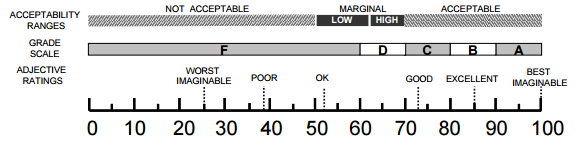
\includegraphics[width=1\textwidth]{fig/eksperimentdesign/sus-score.PNG}
    \caption{SUS karakterskala for å fastslå betydningen av en \acrshort{sus} poengsum \citep{bangor2009determining}}
    \label{fig:sus}
\end{figure}

Bangor et al.\citep{bangor2009determining} har foreslått en karakterskala for å fastslå betydningen av \acrshort{sus}-poengsummen, se figur~\ref{fig:sus}. I følge denne karakterskalaen er et system med en \acrshort{sus}-poengsum på over 70 et brukbart system, et system med en poengsum på 75-85 er et bedre system og et system med en poengsum på over 85 er et utmerket system. Denne karakterskalaen vil bli brukt i analysen av resultatene av forsøkene. Denne skalaene vil bli brukt for å vurdere brukbarheten til pakningsvedleggene og Mine Medisiner. 

\subsection{Reaction cards} \label{sec:reactionCards}
Reaction cards er en måte å få frem negative og positive meninger fra deltakeren om deres meninger om systemet, samt skape diskusjon mellom observerer og deltaker. Reaction cards er et sett med 118 ord som benyttes til diskusjon av systemer ved brukbarhetstesting. I dette eksperimentet ble bare 39 av disse ordene benyttet. Ordene som ble valgt ut var de vi anså som mest aktuelle for de to systemene, og den sammenligningen vi skal gjøre. En mulig feilkilde til resultatene er at vi har valgt ut for mye av samme typen ord. Det at deltakerene ofte gir positive tilbakemeldinger etter brukertester er også en mulig feilkilde \citep{MeasuringSatisfaction, MeasuringDesirability}. For å motvirke dette sørget vi for at minst 40\% av ordene var negativt ladet.

Ved analyse av reaction card-delen av forsøket vil frekvensen av ordene vil bli beregnet og sammelignet for de to systemene.    



\clearpage
\chapter{Resultat}\label{chap:resultat}

Forrige kapittel presenterte gjennomføring av eksperimentet. Eksperimentet besto av to forsøk hvor en gruppe deltakere gjennomførte forsøket ved hjelp av den digitale prototypen Mine Medisiner og en annen gruppe ved hjelp av pakningsvedlegg. Dette kapittelet presenterer resultatet av eksperimentet og danner grunnlaget for analysen som følger i neste kapittel.

\section{Demografi}

\begin{table}[H]
    \centering
    \begin{tabular}{ | p{3.4cm} | p{3.7cm} | p{3.7cm} |  }
      \hline
        & \textbf{Mine Medisiner} & \textbf{Pakningsvedlegg} \\ \hline
        Alder gj.snitt & 34,5 år & 37,8 år \\ \hline
        Kjønnsfordeling & 4 kvinner - 2 menn  & 4 kvinner - 3 menn \\ \hline
        Ant. legemidler totalt & 10 & 8\\ \hline
        Ant. legemidler gj.snitt &  1,67 & 1,14\\ \hline
        Utdanningsnivå & 2 bachelor (2 IT), 2 master (0 IT), 2 phd (1 IT) & 1 vgs, 4 bachelor (3 IT), 1 master (0 IT), 1 phd (1 IT)\\ \hline
        Datakunnskap gj.snitt & 4,5 av 5 &  4,1 av 5 \\ \hline
    \end{tabular}
    \caption{Demografi}
    \label{tab:demografisammenligning}
\end{table}

Tabell~\ref{tab:demografisammenligning} viser en oversikt over de demografiske fordelingen i forsøksgruppene. Folk i alderen 23 til 70 var representert i begge forsøkene. Aldersgruppen 20-30 år var overrepresentert, noe som førte til lav gjennomsnittsalder for begge forsøkene. 

Det var en liten overvekt av kvinner i begge forsøkene. 

Ingen av deltakerne i eksperimentet brukte mer enn tre legemidler fast, og flere brukte ingen legemidler. Legemiddelforbruket i forsøksgruppen til Mine Medisiner var litt høyere enn i forsøksgruppen til pakningsvedlegg. 

Utdanningsnivået var generelt høyt blant deltakerne, men var i snitt høyere blant deltakergruppen til Mine Medisiner. De fleste deltakerene anså seg selv for å ha god datakunnskap. Dette kan henge sammen med utdanningsnivået blant deltakerne, og at mange av brukerne ble rekruttert fra Institutt for datateknikk og informasjonsvitenskap\footnote{http://www.ntnu.no/web/idi/institutt-for-datateknikk-og-informasjonsvitenskap} ved NTNU. 


\section{Forkunnskap}
\label{sec:forkunnskap}
Deltakerene hadde generelt lav forkunnskap om legemidler. Svært få visste mer om de aktuelle legemidlene enn at Ibux var smertestillende. Betydningen av begrepet \textit{interaksjon} i forbindelse med legemidler var uklart for de fleste deltakerene. 

Det var ingen tydelig sammenheng mellom forkunnskap og hvor riktig deltakerne svarte på utsagnene i forsøket. Det var heller ingen tydelig sammenheng mellom forkunnskap og hvor lang tid deltakerne brukte på å besvare utsagnene.

\section{Vurdering av utsagnene}
Ved hjelp av de respektive systemene tok deltakerene stilling til 7 utsagn. Tabell~\ref{tab:PaastanderPak} og tabell~\ref{tab:PaastanderMed} viser tid og fordeling mellom riktige og gale svar for hvert kasus. De to siste radene i hver tabell viser gjennomsnitt og standardavvik for de ulike variablene. 

\begin{table}[H]
    \centering
    \begin{tabular}{ | p{2cm} | p{2cm} | p{2cm} | p{2cm} | p{2cm} | }
      \hline
       \textbf{Deltaker nr.} & \textbf{Tid (mm:ss)} & \textbf{Prosent riktig} & \textbf{Prosent galt} & \textbf{Prosent "vet ikke"} \\ \hline
        1 & 10:38 & 100\% & 0\% & 0\% \\ \hline
        2 & 10:11 & 57\% & 29\% & 14\% \\ \hline
        4 & 13:30 & 43\% & 14\% & 43\% \\ \hline
        5 & 26:54 & 57\% & 29\% & 14\% \\ \hline
        6 & 11:17 & 86\% & 14\% & 0\% \\ \hline
        12 & 04:33 & 100\% & 0\% & 0\% \\ \hline
        13 & 36:51 & 100\% & 0\% & 0\% \\ \hline \hline
        \textbf{Gj.snitt} & 16:16 & 78\% & 12\% & 10\% \\ \hline
        \textbf{Std.avvik} & 11:22 & 25\% & 13\% & 16\% \\ \hline
    \end{tabular}
    \caption{Vurdering av utsagnene ved hjelp av pakningsvedlegg}
    \label{tab:PaastanderPak}
\end{table}


\begin{table}[H]
    \centering
    \begin{tabular}{ | p{2cm} | p{2cm} | p{2cm} | p{2cm} | p{2cm} | }
      \hline
       \textbf{Deltaker nr.} & \textbf{Tid (mm:ss)} & \textbf{Prosent riktig} & \textbf{Prosent galt} & \textbf{Prosent "vet ikke"} \\ \hline
        3 & 03:29 & 100\% & 0\% & 0\% \\ \hline
        7 & 04:47 & 71\% & 0\% & 29\% \\ \hline
        8 & 05:39 & 100\% & 0\% & 0\% \\ \hline
        9 & 07:26 & 86\% & 14\% & 0\% \\ \hline
        10 & 03:51 & 86\% & 0\% & 14\% \\ \hline
        11 & 08:00 & 86\% & 0\% & 14\% \\ \hline \hline
        \textbf{Gj.snitt} & 05:32 & 88\% & 2\% & 10\% \\ \hline
        \textbf{Std.avvik} & 01:52 & 11\% & 6\% & 12\% \\ \hline
    \end{tabular}
    \caption{Vurdering av utsagnene ved hjelp av Mine Medisiner}
    \label{tab:PaastanderMed}
\end{table}

\section{Læringsutbytte}
Tabell~\ref{tab:LaeringsPak} og tabell~\ref{tab:LaeringsMed} viser resultatet av spørsmålene som undersøkte læringsutbytte. Tabellene viser i hvilken grad deltakerne klarte å gjengi informasjon de brukte til å besvare utsagnene. Den viser også hvor mye deltakerne lærte utover svarene på utsagnene. Resultatene tar høyde for forkunnskapene til deltakerene ved å bare gi poeng for kunnskap som ikke ble nevnt i svarene på spørsmålene om forkunnskap, jf.~\ref{sec:forkunnskap}. Gjengitt kunnskap kan gi opp til 3 poeng og lært kunnskap kan gi opp til 6 poeng.

\begin{table}[H]
    \centering
    \begin{tabular}{ | p{2.6cm} | p{2.6cm} | p{2.6cm} | }
      \hline
       \textbf{Deltaker nr.} & \textbf{Ant. gjengitt} & \textbf{Ant. lært}\\ \hline
        1 & 1/3 & 0/6\\ \hline
        2 & 0/3 & 1/6 \\ \hline
        4 & 0/3 & 1/6 \\ \hline
        5 & 0/3 & 0/6 \\ \hline
        6 & 1/3 & 1/6\\ \hline
        12 & 3/3 & 2/6\\ \hline
        13 & 1/3 & 2/6 \\ \hline
        \textbf{Gj.snitt} & 0,86 & 0,86 \\ \hline
        \textbf{Std.avvik} & 0,69 & 1,07 \\ \hline
    \end{tabular}
    \caption{Læringsutbytte for pakningsvedlegg}
    \label{tab:LaeringsPak}
\end{table}


\begin{table}[H]
    \centering
    \begin{tabular}{ | p{2.6cm} | p{2.6cm} | p{2.6cm} | }
      \hline
       \textbf{Deltaker nr.} & \textbf{Ant. gjengitt}   & \textbf{Ant. lært}\\ \hline
        3 & 2/3 & 0/6\\ \hline
        7 & 1/3  & 1/6\\ \hline
        8 & 3/3 & 0/6\\ \hline
        9 & 1/3  & 0/6\\ \hline
        10 & 1/3  & 1/6 \\ \hline
        11 & 1/3 & 0/6\\ \hline
        \textbf{Gj.snitt} & 0,33 (14\%) & 1,67 (29\%) \\ \hline
        \textbf{Std.avvik} & 0,52 (6\%) & 0,52 (56\%) \\ \hline
    \end{tabular}
    \caption{Læringsutbytte for Mine Medisiner}
    \label{tab:LaeringsMed}
\end{table}

\section{SUS}
Alle deltakerene fylte ut \acrshort{sus}-skjema etter å tatt stilling til utsagnene. Poengsummen er beregnet etter \acrshort{sus}-standard, jf. delkapittel~\ref{subsec:SUS}. \acrshort{sus}-poengsummene til de to systemene er gjengitt i tabell~\ref{tab:SUS}.

\begin{table}[H]	
	\centering
\begin{subtable}[b]{2in}
    \centering
    \begin{tabular}{ | p{2cm} | p{2cm} | }
      \hline
       \textbf{Deltaker nr.} & \textbf{Poengsum} \\ \hline
        1 & 55\\ \hline
        2 & 67,5 \\ \hline
        4 & 50 \\ \hline
        5 & 57,5 \\ \hline
        6 & 37,5 \\ \hline
        12 & 67,5 \\ \hline
        13 & 27,5\\ \hline \hline
        \textbf{Gj.snitt} & 51,79\\ \hline
        \textbf{Std.avvik} & 14,91 \\ \hline
    \end{tabular}
    \caption{Pakningsvedlegg}
    \label{tab:SUSPak}
\end{subtable}
\quad
\begin{subtable}[b]{2in}
    \centering
    \begin{tabular}{ | p{2cm} | p{2cm} | }
      \hline
       \textbf{Deltaker nr.} & \textbf{Poengsum} \\ \hline
        3 & 87,5\\ \hline
        7 & 80\\ \hline
        8 & 95\\ \hline
        9 & 95\\ \hline
        10 & 75\\ \hline
        11 & 80\\ \hline \hline
        \textbf{Gj.snitt} & 85,42\\ \hline
        \textbf{Std.avvik} & 8,43 \\ \hline
    \end{tabular}
    \caption{Mine Medisiner}
    \label{tab:SUSMineMed}
\end{subtable}
 \caption{SUS-poengsum}\label{tab:SUS}
\end{table}

\section{Reaction Card}
Fra en forhåndsdefinert liste med ord valgte deltakerne de 5 ordene de mente best beskrev det systemet de brukte, jf. ~\ref{sec:reactionCards}. Ordskyene i figur~\ref{fig:ordskyP} og figur~\ref{fig:ordskyMM} viser hvilke ord som ble brukt for å beskrive hvert system. Størrelsen på ordene indikerer hvor mange som valgte hvert ord. Ordenes frekvens er gjengitt i tabell~\ref{tab:reactionPak} og tabell~\ref{tab:reactionMed}. 

\begin{figure}[H]
    \centering
    
\includegraphics[width=0.8\textwidth]{fig/resultat/ordskyP.png}
    \caption{Ordsky for Reaction Card-oppgave Pakningsvedlegg}
    \label{fig:ordskyP}
\end{figure}

\begin{figure}[H]
    \centering
    
\includegraphics[width=0.8\textwidth]{fig/resultat/ordskyMM.png}
    \caption{Ordsky for Reaction Card-oppgave MineMedisiner}
    \label{fig:ordskyMM}
\end{figure}


\begin{table}
	\centering
	\begin{subtable}[b]{2in}
		\centering
    \begin{tabular}{ | p{2.5cm} | p{1.7cm} | }
      \hline
       \textbf{Ord} & \textbf{Frekvens} \\ \hline
        Nyttig			&		4\\ \hline
        Lett å bruke	&		4\\ \hline
        Intuituv		&	    3\\ \hline
        Enkelt			&		3\\ \hline
        Forståelig		&		4\\ \hline
        Spennende		&		3\\ \hline
        Troverdig		&		1\\ \hline
        Relevant		&		3\\ \hline
        Tilfredsstillende	&	1\\ \hline
        Personlig			&	1\\ \hline
        Tidsbesparende		&	2\\ \hline
        Effektiv			&	1\\ \hline
    \end{tabular}
    \caption{Pakningsvedlegg}
    \label{tab:reactionPak}
	\end{subtable}
	\quad
	\begin{subtable}[b]{2in}
		\centering
    \begin{tabular}{ | p{2.5cm} | p{1.7cm} | }
      \hline
       \textbf{Ord} & \textbf{Frekvens} \\ \hline
        Verdifull			&		3 \\ \hline
        Nyttig				&   	5\\ \hline
        Tidkrevende			&		5\\ \hline
        For teknisk			&		2\\ \hline
        Ineffektiv			&		1\\ \hline
        Relevant			&		3\\ \hline
        Pålitelig			&		1\\ \hline
        Treg				&   	1\\ \hline
        Kompleks			&		2\\ \hline
        Overveldende		&		3\\ \hline
        Troverdig			&		1\\ \hline
        Avansert			&		1\\ \hline
        Upersonlig			&		2\\ \hline
        Ineffektiv			&		1\\ \hline
        Forståelig			&		1\\ \hline
        Frustrerende		&		1\\ \hline
        Forvirrende			&		1\\ \hline
        Stressende			&		1\\ \hline
    \end{tabular}
    \caption{Mine Medisiner}
    \label{tab:reactionMed}
    \end{subtable}
    \caption{Ordfrekvens fra Reaction Cards}\label{table:Ordsky}
\end{table}
\chapter{Analyse}\label{chap:analyse}
Dette kapittelet presenterer fire påstander som underbygges av resultatene i  kapittel~\ref{chap:resultat}. 


\section[Tidsbruk]{Bruk av Mine Medisiner er raskere enn bruk av pakningsvedlegg}
Gjennomsnittstiden for å ta stilling til de syv utsagnene for deltakergruppen til Mine Medisiner var 5:32, mot 16:16 for deltakergruppen til pakningsvedlegg. Differansen er stor. Tidsbruken gir imidlertid lite informasjon når den vurderes alene fordi raskere gjennomføring kan ha ført til flere feil ved besvaring av utsagnene. Det er derfor interessant å se på tidsbruket i sammenheng med antall riktige svar når man vurderer hvor rask deltakerne er til å ta stilling til utsagnene. Total tid og tid per riktig svar er gitt i tabell~\ref{tab:tidperrettMed}. Tabellen viser at tiden per riktige svar er mye lavere for Mine Medisiner, enn for pakningsvedlegg. 

Ut ifra tabellene ser det ut til at bruken av Mine Medisiner er raskere enn bruken av pakningsvedlegg. For pakningsvedlegg varierete det mye hvor lang tid deltakerne brukte per riktige svar. Så store forskjeller i et forsøk med så få deltakere gjør det vanskelig å si noe om trender i tidsbruk.

\todo{Lage figur som viser overlapp std.avvik}

\begin{table}[H]
    \centering
    \begin{tabular}{ | p{2cm} | p{3cm} |  p{3cm} |  }
      \hline
       \textbf{Deltaker nr.} & \textbf{Tid totalt} & \textbf{Tid per riktige}\\ \hline
        1 & 10:30  &1:31\\ \hline
        2 & 10:11 &2:33\\ \hline
        4 & 13:30  &4:30\\ \hline
        5 & 26:54  &6:44\\ \hline
        6 &  11:17 & 1:53\\ \hline
        12 & 4:33 & 00:39\\ \hline
        13 & 36:51 &5:16\\ \hline \hline
        \textbf{Gj.snitt} & 16:16 & 03:18 \\ \hline
        \textbf{Std.avvik} & 11:22 & 02:13\\ \hline
    \end{tabular}
    \caption{Tid per riktige svar ved bruk av pakningsvedlegg}
    \label{tab:tidperrettPak}
\end{table}

\begin{table}[H]
    \centering
    \begin{tabular}{ | p{2cm} | p{3cm} |   p{3cm} | }
      \hline
       \textbf{Deltaker nr.} & \textbf{Tid totalt} & \textbf{Tid per riktige} \\ \hline
        3 & 03:29 & 00:30\\ \hline
        7 & 04:47 & 00:57\\ \hline
        8 & 05:39 & 00:48\\ \hline
        9 &  07:26 & 1:14\\ \hline
        10 & 03:51 & 00:39\\ \hline
        11 & 08:00 & 1:20\\ \hline \hline
        \textbf{Gj.snitt} & 5:32 & 00:55 \\ \hline
        \textbf{Std.avvik} & 1:52 & 00:20  \\ \hline
    \end{tabular}
    \caption{Tid per riktige svar ved bruk av Mine Medisiner}
    \label{tab:tidperrettMed}
\end{table}

Vi undersøkte om demografiske forskjeller påvirket hvor lang tid deltakerene brukte på å ta stilling til utsagnene. Antagelsen var at alder og utdanningsnivå ville påvirke deltakernes tidsbruk. For eksempel ved at at de over 65 kom til å bruke lenger tid, og at dette måtte tas hensyn til i analysen ved å trekke fra den ekstra tiden som kunne skyldes alder. Det var imidlertid ikke noe som tydet på at demografi påvirket hvor raske deltakerene var, og vi så derfor bort ifra demografien i analysen av tidsbruken.

Halvparten av deltakerne i gruppen til Mine Medisiner hadde utdanning innen IT. Selv om det ikke er noe i resultatene som tyder på at utdanning innen IT gjorde at deltakerne tok stilling til utsagnene raskere, kan disse deltakerne lettere ha forstått hvordan grensesnittet fungerte. Dette kan ha ført til at gjennomsnittstiden ble lavere enn den ville blitt for et mer representativt utvalg deltakere. Et utsagn fra en av deltakerne: \begin{quote} \textit{ “Det er forståelig fordi brukergrensesnittet er kjent, og ligner på mange andre grensesnitt'' } \end{quote}

Ordene som ble brukt for å beskrive bruken av pakningsvedlegg viste tydelig at opplevelsen var preget av at det tok lang tid å vurdere utsagnene. Ord som gikk igjen var \textit{tidkrevende, ineffektiv og treg}. Begrunnelsen deltakerne gav var at det var store mengder informasjon det tok lang tid å lese på grunn av vanskelig språk og manglende struktur. Et utsagn fra en av deltakerne: \begin{quote} \textit{ “Det tar tid å lese gjennom hele pakningsvedlegg. Til slutt orker man ikke å lese alt og bare skummer igjennom.'' } \end{quote}

Mine medisiner ble beskrevet som \textit{tidsbesparende og effektiv}. Dette forklarte deltakerne med at all relevant informasjon var samlet på ett sted, og at det var enkelt å få oversikt. 

\textbf{Analysen førte til påstanden: \textit{Bruk av Mine Medisiner er raskere enn bruk av pakningsvedlegg}. Tendenser i tidsbruken underbygger påstanden, men på grunn av høye standardavvik kan vi ikke påstå at det er “mye`` raskere å bruke Mine Medisiner enn pakningsvedlegg. }

\section[Riktighet]{Utsagn vurderes mer riktig ved bruk av Mine Medisiner, enn ved bruk av pakningsvedlegg}
Syv utsagn ble tatt stilling til i forsøkene. Tabell~\ref{tab:PaastanderPak} og tabell~\ref{tab:PaastanderMed} i kapittel~\ref{chap:resultat} viser andel riktige vurderinger for henholdvis pakningsvedlegg og Mine Medisiner. I gjennomsnitt vurderte deltakerene i forsøket med Mine Medisiner 88\% av utsagnene riktig, mot 78\% for deltakerne til pakningsvedlegg. Forskjellen mellom andelen riktige svar ved bruk av Mine Medisiner og pakningsvedlegg faller innenfor standardavvikene, og resultatet er dermed ikke signifikant. 

Deltakerene som brukte Mine Medisiner gjorde færre feilvurderinger enn de som brukte pakningsvedlegg. Snittet for antall feil var 2\% for Mine Medisiner, mot pakningsvedlegg med 12\% feil. Forskjellene er imidlertid ikke store nok til å falle utenfor standardavvikene. 

Det er ikke mulig å si om visualisering av informasjon direkte førte til at utsagnene ble vurdert mer riktig ved bruk av Mine Medisiner enn ved bruk av pakningsvedlegg, men tilbakemeldinger fra deltakerene kan tyde på at visualiseringen spilte en rolle. Deltakerne beskrev Mine Medisiner som intuitiv og og forståelig. Flere fremhevet at interaksjonsgrafen~\ref{fig:interaksjonsGraf} gjorde det enkelt å finne informasjon om interaksjoner: \begin{quote} \textit{ “Det var litt kult med den grafen, den var fancy. Det var enkelt å se hvordan alle legemidlene fungerte sammen.'' } \end{quote}

Som tidligere nevnt hadde halvparten av deltakerene i forsøket med Mine Medisiner utdanning innen \acrshort{it}. Innenfor denne fagdisiplinen er grafer er et vanlig verktøy for å visualisere informasjon. Et utvalg deltakere med god kjennskap til grafer kan ha ført til bedre forståelse av informasjonen som ble visualisert i en graf i Mine Medisiner, enn det som ville vært tilfelle for et mer representativt utvalg deltakere. 

Pakningsvedleggene ble oppfattet som vanskelige å bruke. Begrunnelsen var at pakningsvedleggene inneholdt mye informasjon som ikke var personlig tilpasset og at språket var tungt. Tilbakemeldinger fra deltakerene tyder på at tungt språk, mye informasjon og liten grad av personlig tilpasning kan være viktige faktorer til at pakningsvedlegg kom dårligere ut enn Mine Medisiner:


\begin{quote} \textit{ ``Nei, jeg skjønner veldig godt at jeg ikke liker pakningsvedlegg. Kanskje ville pakningsvedleggene sagt meg mer hvis jeg hadde kunne litt mer om legemidler og hvilke gruppe de tilhører. Men for den vanlige mannen i gaten er dette håpløst.'' } \end{quote}

\begin{quote} \textit{ ``Det står så mye som folk uten utdannelse innen medisin ikke forstår noe av. '' } \end{quote}

\begin{quote} \textit{ ``....menstruasjonssmerter er jo ikke så interessant for meg.'' } \end{quote}

\begin{quote} \textit{ ``Dette er veldig upersonlig. Jeg vil gjerne vite hva som gjelder for meg og ikke bare for folk generelt.'' } \end{quote}

\begin{quote} \textit{ ``Du må forstå litt legeting for å forstå pakningsvedlegget.'' } \end{quote}

\begin{quote} \textit{ ``Det er tungvindt å lese når det står så mye.'' } \end{quote}

\begin{quote} \textit{ ``Jeg klarer ikke å finne ut av interaksjoner ut i fra pakningsvedleggene. Det er så mye ord og uttrykk jeg ikke forstår.'' } \end{quote}


Utsagn vurderes mer riktig ved bruk av Mine Medisiner, enn ved bruk av pakningsvedlegg
----> Pasienter vurderer legemiddelsituasjon riktigere 

\textbf{Analysen førte til påstanden: \textit{Pasienter 
vurderer egen legemiddelsituasjon riktigere
gjør mer riktige vurderinger
forstår legemiddelinformasjon bedre
...ved bruk av Mine Medisiner, enn ved bruk av pakningsvedlegg}}


\section[Læringsutbytte]{Pasienter kan lære litt om egne legemidler både ved bruk av pakningsvedlegg og ved bruk av Mine Medisiner}
Det er mange måter å definere \textit{læring}. En form for læring er å huske informasjon slik at den kan gjengis. En annen form for læring er å oppdage ny informasjon. 

5 av 7 deltakerne i forsøket med pakningsvedlegg lærte noe utover utsagnene de skulle besvare, jf~\ref{tab:LaeringsPak}, mot 2 av 6 deltakerne med Mine Medisiner, jf~\ref{tab:LaeringsMed}. 
Selv om mange deltakere lærte noe, lærte hver deltaker veldig lite. Hver deltaker kunne få seks poeng for ny læring. Gjennomsnittet for læring av ny informasjon ved bruk av pakningsvedlegg var 0,86 poeng, tilsvarende 14\% av mulige poeng. For Mine Medisiner var gjennomsnittet 0,33 poeng, som tilsvarer 6\%. Læringen av ny informasjon var veldig lav i begge forsøken, men den var høyere ved bruk av pakningsvedlegg. 

Deltakerne i forsøket med Mine Medisiner kunne gjengi litt mer informasjon fra vurderingen av utsagnene, enn deltakerene i forsøket med pakningsvedlegg. Hver deltaker kunne få tre poeng for å gjengi informasjon, Gjennomsnittet i forsøket med pakningsvedlegg var 0,86 som tilsvarer 28\% av mulige poeng. For Mine Medisiner var snittet 1,67, som tilsvarer 56\%.

Eksperimentet tyder på at Mine Medisiner og pakningsvedlegg fører til forskjellige former for læring. Ved bruk av Mine Medisiner var deltakerenes evne til å gjengi informasjon høyere enn ved bruk av pakningsvedlegg. Deltakerenes evne til å lære ny informasjon var høyere ved bruk av pakningsvedlegg, enn ved bruk av Mine Medisiner. Generelt var læringsutbytte lav for begge systemene. Det gjaldt begge former for læring, både å gjengi informasjon og å oppdage ny informasjon.

Vi undersøkte om antall legemidler deltakerne brukte påvirket evnen til å tilegne seg kunnskap om legemidler. Antagelsen var at de deltakerne som brukte legemidler fast ville lære mer om legemidlene. Det var imidlertid ikke noe som tydet på at dette var tilfellet, og vi tok derfor ikke hensyn til antall legemidler i vurderingen av hvor mye hver deltaker lærte. 

\section[Brukbarhet]{Mine Medisiner har mye bedre brukbarhet enn pakningsvedlegg}
Poengsummen til \acrshort{sus}-skjemaene brukes til å vurdere hvor brukbart et system er. Som nevnt i delkapittel~\ref{subsec:SUS} regnes et system som brukbart hvis det har en \acrshort{sus}-poengsum på over 70, som et bedre system hvis det hat en poengsum på 75-85, og som et utmerkede systemer hvis det har en poengsum på over 85. 

\acrshort{sus}-poengsummen for pakningsvedlegg er gjengitt i tabell~\ref{tab:SUSPak}, og Mine Medisiner i tabell~\ref{tab:SUSMineMed}. Mine Medisiner har en signifikant bedre \acrshort{sus}-poengsum enn pakningsvedleggene. Mine Medisiner regnes som et utmerket system med en gjennomsnittlig poengsum på over 85, mens pakningsvedlegg har en så lav poengsum at det ikke er regnet som brukbart. 

Figur~\ref{fig:ordskyP} og figur~\ref{fig:ordskyMM} viser at deltakerne som brukte Mine Medisiner valgte mer positive ord enn deltakerne som brukte pakningsvedleggene i reaction card-delen. Dette underbygger påstanden om at Mine Medisiner er mer brukbar enn pakningsvedlegg. 

Ved å se på forklaringene deltakerne gav for ordene de valgte kan noen trender sees for hva deltakerne forklarte forskjellen i brukbarhet med.

Forklaringene deltakerene gav på valg av ord gir et inntrykk av hva som gjør Mine Medisiner mer brukbar enn pakningsvedlegg. Det ble blant annet nevnt at pakningsvedlegg var upersonlig, brukte tungt språk og at de inneholdt for mye informasjon. Deltakerne forklarte at Mine Medisiner var logisk oppbygd, og at det var lett å forstå informasjonen som ble presentert. Flere av deltakerene trakk frem at de synes en grafisk fremstilling av interaksjoner gjorde det enkelt å få oversikt. 
\chapter{Diskusjon} \label{chap:diskusjon}
Forrige kapittel presenterte analysen av resultatene for forskningen. I dette kapittelet diskuteres valgene vi har tatt, hvilke utfordringer vi har møtt underveis og gyldighetene av resultatene. 

\todo{diskutere demografi}

\section{Gjennomføringen av eksperimentet}
I de neste avsnittene diskuteres valgene vi har tatt, og hvilke alternative fremgangsmåter som kunne vært benyttet. Utfordringer som har oppstått underveis og hvordan vi har valgt å løse dem vil også bli diskutert her. 

Eksperimentet kunne blitt mer reellt ved å sammenligne et "ferdig" system med pakningsvedlegg, istedenfor en prototype. Det kunne blitt utført et forsøk i reelle situasjoner på et ferdig system, hvor deltakerene var faktiske brukere. Brukerene kunne fått tilgang til systemet hjemme, lagt inn sin egen legemiddelliste, og brukt systemet i hverdagen. Vi kunne samlet informasjon om bruk av pakningsvedlegg og Mine Medisiner over tid. På den måten kunne brukerene benyttet systemene i mer realistiske brukskontekster, og vi ville da også øke validiteten av resultatene våre.  

Begrensinger i tid og kapasitet gjorde det imidlertid ikke gjennomførbart å utvikle et ferdig system. For å i størst mulig grad ligne et ferdig system ble det utviklet en digital prototype til eksperimentet. 

På grunn av føringene forskningsspørsmålet gav ble det valgt å gjennomføre et forsøk som sammenlignet en digital prototype og pakningsvedlegg. Forskningsspørsmålet kunne vært formulert annerledes. Ved å fokusere mer på å sammenligne graf med tekst istedenfor å sammenligne Mine Medisiner med pakningsvedlegg, kunne noen variabler i forsøket antageligvis blitt eliminert. 

Ved å gjennomføre forsøkene kun på \acrshort{tia}\footnote{TIA: Hjerneslag hvor symptomene trekker seg tilbake i løpet av 24 timer}-pasienter kunne flere variabler blitt eliminert: Alder hadde blitt jevnere, forkunnskap og kjennskap til legemiddellisten hadde vært likere og deltakerne hadde hatt en bedre forståelse av konteksten. Det ville økt reliabilitet i eksperimentet vårt. Dessverre var det ikke tid eller kapasitet til å rekruttere fra en så smal brukergruppe. 

Eksperimentet utført i dette prosjektet har sammenlignet to svært forskjellige systemer. For å avklare om interaksjonsgraf og symptomsøk er bedre enn tekst, kunne vi laget en tekstbeskrivelse av den samme informasjonen som er tilgjengelig i Mine Medisiner, og sammenligne denne tekstbeskrivelsen med Mine Medisiner. Da vil forskjellen mellom systemene være mindre, og derfor vil det være færre variabler å ta hensyn til når resultatene skal analyseres. Det ville da ikke vært en sammenligning av pakningsvedlegg og Mine Medisiner, men en sammenligning av måte å presentere informasjon på. Ved å endre pakningsvedleggene på denne måten ville vi ikke fått sammenlignet Mine Medisiner med et eksisterende system, for å vurdere hvor godt det fungerer i forhold til noe pasienter har tilgang til i dag. 

Vi ønsket å knytte eksperimentet til virkeligheten ved å sammenligne en eksisterende kilde til informasjon, med en ny presentasjonsmåte. Dette var for å vurdere om informasjon kan presenteres på en bedre måten enn i dag. Denne sammenligningen ville ikke være reell, dersom relevante utsnitt av pakningsvedleggene hadde blitt konstruert for dette eksperimentet.

Systemene som ble brukt i eksperimentet var svært forskjellige. Pakningsvedlegg er et ferdig system på papirformat, mens Mine Medisiner er en digital prototype. Når to så forskjellige systemer sammenlignes er det vanskelig å vurdere hva som forårsaker resultatene. Det er mange ting som skiller systemene, og som dermed kan føre til at systemene presterer ulikt. 
Hver deltaker fikk bare utføre forsøket på ett av systemene. Dette gjør det vanskeligere å sammenligne systemene fordi ulikheter mellom deltakere kan ha bidratt til ulikhetene i resultatene. At hver deltaker ikke utfører forsøket på begge systemene hindret at deltakerene brukte det de lærte ved å bruke det ene systemet når de skulle bruke det neste. En annen måte å hindre dette på er ved å gjennomføre forsøk på begge systemene for alle deltakerene, men ha forskjellige oppgaver på de to systemene. Dette fører imidlertid til flere usikkerhetsmomenter i vurderingen fordi det er vanskelig å lage oppgaver som går ut på de sammen tingene med samme vanskelighetsgrad.

Forsøkene tok ca en time å gjennomføre, og det var mange variabler som påvirket forsøkene. At forsøkene var så omfattende gjorde at det bare var mulig å gjennomføre 13 forsøk totalt. Dersom hvert forsøk hadde vært mindre omfattende kunne det blitt gjennomført flere forsøk, og det hadde vært færre variabler å ta hensyn til under analysen av resultatene. Gjennomføring av flere forsøk ville kunne gitt bedre grunnlag for statistisk analyse, men kunne gått på bekostning av innsikt i den enkelte deltakers vurderinger. 


\section{Gyldighet av resultater}
Det er viktig å ta høyde for eventuelle feilkilder som kan ha ført til ugyldige resultater. I de neste avsnittene diskuteres styrken på resultatene, og hvilke faktorer som styrker eller svekker påliteligheten av dem. 

Det ble gjennomført henholdsvis 6 og 7 forsøk av hvert system. Utvalget er for lite til å gjøre statistisk analyse av resultatene. For å motvirke at tilfeldigheter påvirket resultatene kunne det vært gjennomført flere forsøk. Mye tyder på at analysen stemmer fordi det er et mønster i resultatet til forsøkene som er gjennomført, men det lave antallet forsøk gjør at grunnlaget for analysen var tynt. 

Utdanningsnivået til deltakerne er ikke representativt for befolkningen. 12 av 13 av deltakerne hadde høyere utdanning, mot ca 50 \% av befolkningen generelt. Dette gjorde at den ytre validiteten til forsøket ble svekket. Det høye utdanningsnivået har påvirket begge gruppene, fordi snittet av utdanningsnivå i de to gruppene var relativt likt. 

Fordi Mine Medisiner er et datasystem, kan forsøket hvor deltakerene fikk bruke Mine Medisiner ha blitt påvirket i positiv retning av at halvparten av deltakerne hadde utdanning innen \acrshort{it}. I gruppen som utførte oppgaver ved hjelp av pakningvedlegg hadde også halvparten utdanning innen \acrshort{it}, men dette har nok ikke påvirket resultatene i like stor grad. 

Det var store demografiske forskjeller mellom deltakerne, noe som fører til ekstra variabler som kan påvirke resultatet. På grunn av at demografien innad i hver gruppe er relativt lik, er de demografiske forskjellene sett bort i fra i analysen. Det er mulig at demografiske fakta som ikke ble avdekket kan ha påvirket resultatene. 

Pakningsvedlegg var kjent for fleste. Deltakerenes tidligere erfaring med pakningsvedlegg kan ha påvirket svarene de gav, og hvordan de vurderte systemet. 

Vi kan ikke utelukke metodiske svakheter, eller at det finnes forskning som viser til andre resultater enn de vi har funnet.
\chapter{Konklusjon} \label{chap:konklusjon}
I denne masteroppgaven ble det utviklet en prototype som inneholdt en visuell fremstilling av personlig legemiddelinformasjon. Denne ble sammenlignet med pakningsvedlegg i et eksperiment. 

Før vi utførte eksperimentet hadde vi følgende hypoteser:
\begin{enumerate}
 \item Ved å bruke prototypen får pasienter raskere svar på spesifikke spørsmål enn ved å bruke pakningsvedlegg.
 \item Ved å bruke prototypen oppfatter pasienter svaret på spesifikke spørsmål mer korrekt enn ved å bruke pakningsvedlegg.
 \item Ved å bruke pakningsvedlegg tilegner pasienter seg kunnskap utover det de leter etter, i større grad enn ved å bruke prototypen
\end{enumerate}

Resultatene av forsøkene viste at deltakerene raskere fant informasjonen de lette etter ved å bruke prototypen enn ved å bruke pakningsvedlegg. Tilbakemeldingene som kom i Reaction Card-delen av forsøkene fortalte at deltakerene opplevde pakningsvedlegg som tidkrevende og inneffektive, mens de opplevde prototypen som tidsbesparende. I tilbakemeldingene forklarte deltakerene at de trodde det tok lang tid å bruke pakningsvedlegg fordi det var så store mengder informasjon som presenteres i dem. Det tok lang tid å få oversikt over informasjonen og finne det de lette etter. 

Deltakerene svarte mer korrekt på påstander ved å bruke prototypen enn ved å bruke pakningsvedlegg. Når det gjaldt bivirkninger var det flere av deltakerene som ikke fant den informasjonen de trengte i pakningsvedleggene. Det kan skyldes at informasjonen var gjemt bort i mye annen informasjon. Når det gjaldt interaksjoner var det flere av deltakerene som fant informasjonen de trengte i pakningsvedleggene, men som allikevel ikke svarte korrekt på påstandene. Det kan virke som om deltakerene ikke forstod informasjonen som ble presentert. I tilbakemeldingene på Reaction Card delen av forsøkene forklarte deltakerene dette med at pakningsvedleggene brukte komplisert medisinsk terminologi som de ikke forstod. 

Deltakerene var i større grad i stand til å tilegne seg kunnskap utover det de lette etter ved bruk av pakningsvedlegg enn ved bruk av prototypen. Deltakerene var imidlertid i stand til å huske mer av det de lette etter ved bruk av prototypen.


Forskningsspørsmålet for masteroppgaven var: 
\thesisRQ

Prototypen gav pasienter både raskere og mer korrekt kunnskap om interaksjoner og bivirkninger knyttet til egne legemidler enn pakningsvedlegg. Altså kan en visuell fremstilling av personlig legemiddelinformasjon på et digitalt format gi raskere og mer korrekt kunnskap om bivirkninger og interaksjoner enn tekst fra pakningsvedlegg. 

Vi vet imidlertid lite om hva som gjorde at prototypene gav raskere og mer korrekt kunnskap enn pakningsvedlegg. Eksperimentet klarte ikke å vise at tekst gav dårligere eller bedre resultater enn andre alternativer slik som graf og søkefunskjonalitet. Grunnen til at det ikke kan trekkes noen konklusjon om dette er at det var andre faktorer som også skilte systemene. Tungt språk, mye informasjon og liten grad av personlig tilpasning ser ut til å være viktigere faktorer til at pakningsvedlegg kom dårligere ut i eksperimentet.

Tilbakemeldingene fra deltakerene tyder på at prototypen er mer brukbar enn pakningsvedleggene. Høyere brukbarhet kan føre til at pasienter tilegner seg med kunnskap om egne legemidler. 
\chapter{Videre arbeid} \label{chap:videreArbeid}

Dette kapittelet presenterer mulige videreføringer av prosjektet.

I dette prosjektet ble det gjennomført en kvalitativ studie, med få deltakere, som sammenlignet Mine Medisiner med pakningsvedlegg. Forsøket som ble utført gikk i dybden, for å samle informasjon på et smalt felt som ikke er mye undersøkt. En kvalitativ studie kan følges opp med en kvantitativ undersøkelse for å belyse problemområdet fra flere vinkler. En kvantitativ undersøkelse kan etterprøve resultatene og kan styrke validiteten av det som er gjort, dersom resultatene samsvarer. En kvantitativ undersøkelse kan gi bedre forståelse av resultatene som er avdekket i den kvalitative studien ved å sette dem i større sammenheng.

Per i dag gir ingen verktøy oversikt over effekten av egne legemidler, slik Mine Medisiner er ment å gjøre. Resultatet av forsøket vårt var at prototypen for Mine Medisiner gav raskere og mer korrekt informasjon om bivirkninger og interaksjoner enn pakningsvedlegg. Fordi resultatene tyder på at legemiddelinformasjon kan formidles på en bedre måte enn i dag, kan det være hensiktsmessig å videreutvikle Mine Medisiner til et ferdig system. Systemet kan gjøres tilgjengelig for hele befolkningen på for eksempel helsenorge.no, som er den offentlige inngangsporten til helse- og omsorgstjenester på nett. 

Den ferdige versjonen av Mine Medisiner må bygge på en kunnskapsrepresentasjon for å kunne resonnere om legemidler. En kunnskapsrepresentasjon er avhengig av gode kompetansespørsmål for å definere problemområdet og vurdere hvor god kunnskapsrepresentasjonen er. Etter å ha etablert kompetansespørsmålene bør eksisterende kunnskapsrepresentasjoner for legemidler, som for eksempel DrOn, studeres. For å kunne bruke eksisterende kunnskapsrepresentasjoner må de tilpasses og fylles med norske kliniske terminologier fra for eksempel ordnett, ICD10, \acrshort{mesh}, finnkode.no og legemiddelhåndboken. Arbeidet med å fylle kunnskapsrepresentasjonen kan effektiviseres ved å benytte en automatisert prosess for å hente informasjon fra de ulike kildene. 

HAFE-prosjektet, se vedlegg~\ref{HEFE}, er et steg på veien mot å lage en kunnskapsrepresentasjon til bruk i Mine Medisiner. Ontologien i HAFE-prosjektet er god nok til at prototypen til Mine Medisiner kunne brukt den. Ontologien er begrenset til et fåtall brukere og inneholder forenklinger som er tilpasset prototypen. Disse forenklingene gjør imidlertid at ontologien ikke er i stand til å modellere virkeligheten på en tilstrekkelig måte for en ferdig versjon av Mine Medisiner. For at en ontologi skal være god nok for en ferdig versjon av Mine Medisiner må den være komplett og korrekt for hele befolkningen. En slik ontologi bør, i større grad enn i HAFE-prosjektet, baseres på DrOn og andre anerkjente prosjekter. 



%% PART 4 -- referanser
\addcontentsline{toc}{chapter}{Bibliografi}

\printbibliography

\clearpage
	%% Referanser kan endres i "mylib.bib"

%% PART 5 -- vedlegg
\begin{appendices}
\chapter{Lillian 27 år} \label{chap:lillian}
Lillian er en 27 år gammel kvinne som har hatt epilepsi siden hun var 9 år. Hun er samboer med barndomskjæresten sin på det lille tettstedet hvor hun har vokst opp, og jobber på en Rema-butikk i gangavstand fra leiligheten de bor i. Nå ønsker Lillian og samboeren seg barn. Samboeren vil hun bare skal slutte med p-pillene med en gang, mens Lillian er mer usikker, siden hun har hørt så mange historier om hva som kan gå galt. 

Lillian har brukt epilepsimedisin i mange år og vet at noen epilepsimedisiner kan være fosterskadelige. Legen hennes har tidligere sagt at epilepsi-anfall også kan være skadelige for et eventuelt foster. Lillian er veldig usikker og har stort behov for informasjon. Hun har ingen god relasjon til fastlegen sin og har ikke vært i kontakt med spesialisten på sykehuset på nesten tre år, siden det er så lenge siden hun har hatt anfall. Hun lurer blant annet på om hun skal gjøre endringer i legemiddelbruken sin før hun slutter med p-pillene, om hun skal fortsette med de legemidlene hun har eller begynne med nye, om hun bare skal endre dosen eller om hun helt skal slutte med epilepsimedisiner. Noen har også sagt til henne at alle gravide bør ta folsyre i første del av graviditeten og at dette er spesielt viktig for pasienter med epilepsi. Lillians mor har tidligere brukt et B-vitamin-preparat som heter TrioBe. Det inneholder blant annet folsyre, så Lillian har begynt å bruke dette, selv om hun ikke har sluttet med p-pillene ennå. 

Lillian har prøvd ganske mange forskjellige legemidler mot epilepsi opp gjennom årene, men har nå brukt Keppra og Lamictal de siste tre-fire årene. Legemidlene ser ut til å virke godt, hun har ikke hatt epileptiske anfall på neste tre år og hun opplever ingen plagsomme bivirkninger. Lillian tar blodprøver hos fastlegen to ganger i året for å se at hun får riktig dose av de to legemidlene mot epilepsi. Blodprøvesvarene ligger innenfor det såkalte referanseområdet, det vil si at doseringen er godt tilpasset hennes situasjon. 

\textbf{Legemidler:}
\begin{itemize}
\item Keppra (levetiracetam) tabletter 1500 mg 2 ganger daglig MOT EPILEPSI
\item Lamictal (lamotrigin) tabletter 100 mg 2 ganger daglig MOT EPILEPSI
\item Yasmin tabletter 1 daglig P-PILLER
\item Ibux tabletter 400 mg 1 tablett inntil 3 ganger daglig MOT HODEPINE 
\item TrioBe tabletter 1 daglig B-VITAMINTILSKUDD
\end{itemize}

Lillian tar begge legemidlene mot epilepsi regelmessig og slik hun har fått beskjed om. Hun er opptatt av å ikke få nye anfall, både fordi hun opplever det som ubehagelig, men også fordi hun bor «litt langt fra alt og alle» og er avhengig av å kunne kjøre bil. Legemidler mot epilepsi kan i tillegg være fosterskadelige. Epileptiske anfall kan også være skadelige – både for barnet og for moren. Det er derfor viktig med god informasjon og planlegging når pasienter med epilepsi ønsker å bli gravide. 

Ibux har Lillian fått på resept fra fastlegen sin for snart et år siden. Hun ønsket selv utredning for migrene, men fastlegen mente det i første omgang var nok å gi henne smertestillende uten videre undersøkelser. Lillian føler seg litt avspist av fastlegen og har ikke tatt kontakt med ham mer, selv om hun fortsatt ofte opplever sterke hodepine og tar Ibux nesten hver dag. Bruk av smertestillende legemidler som f.eks. Ibux over lenger tid, kan virke mot sin hensikt og faktisk gi hodepine. En kan ikke si sikkert at det er tilfelle for Lillian, men det kan ikke utelukkes. Bruk av Ibux og lignende legemidler er heller ikke gunstig for kvinner som ønsker å bli gravide elle er gravide. Lillian bør slutte med Ibux. 

TrioBe har Lillian fått av sin mor. Det inneholder riktignok 0,8 mg folsyre, men også to andre B-vitaminer som Lillian i utgangspunktet ikke trenger. Kvinner som bruker den typen legemidler mot epilepsi som Lillian gjør, bør bruke 1 mg folsyre daglig gjennom hele svangerskapet. Lillian bør derfor slutte med TrioBe og begynne med tabletter som inneholder 1 mg folsyre og ikke noe annet.


\chapter{Lars 57 år} \label{chap:lars}

Lars er 57 år og jobber som mellomleder i en større bedrift. Han er gift og har tre barn. Lars er travelt opptatt med jobb, trener mye og har akkurat kjøpt seg hytte på fjellet som han pusser opp og utvider i ledige stunder. Lars og kona har tre engelsksettere som de går på fuglejakt med om høsten, men som ellers stort sett er plassert i kennel. 

Lars har alltid vært i god form og aldri brukt legemidler fast unntatt Nicorette da han sluttet å røyke for noen år siden. Han har brukt mye kosttilskudd tidligere, men har sluttet med det etter at han måtte begynne med blodfortynnende medisin.

Lars har nettopp gjennomgått et større hjerteinfarkt og føler seg ganske redusert fortsatt. Han fikk også konstatert hjerteflimmer. Lars kjenner seg nedfor og kona som er sykepleier lurer på om han kan ha fått depresjon som en bivirkning av blodtrykksmedisinen han har begynt med. Han er også plaget med impotens og mareritt.

Legen på sykehuset var svært tydelig da han snakket med Lars og ga beskjed om at han måtte bruke flere legemidler resten av livet for å hindre nye hjerteinfarkt. Lars, som ellers er vant til å lede diskusjoner og være den som gir andre ordre, ble litt «satt ut» og fikk seg ikke til å stille spørsmålstegn ved noe av det legen sa eller å spørre om utdypende informasjon om legemidlene han fikk skrevet ut.  

Lars har forsøkt å lete seg frem til informasjon om legemidlene sine på nettet, men kona sier han ikke må tro på mesteparten av det han finner, det er bare skremselspropaganda. Hun leser høyt for ham fra Felleskatalogen uten at det gir ham spesielt mye mer forståelse. 

\textbf{Legemidler:}
\begin{itemize}
\item Marevan tabletter 2,5 mg Tas etter egen liste BLODFORTYNNENDE
\item Selo-zok tabletter 100 mg 1 daglig BLODTRYKKSSENKENDE
\item Renitec tabletter 10 mg 1 daglig BLODTRYKKSSENKENDE
\item Simvastatin tabletter 40 mg 1 kveld KOLESTEROLSENKENDE
\end{itemize}

Lars får standardbehandling for å forebygge nye hjerteinfarkt og annen hjerte-kar-sykdom. Både depresjon, impotens og mareritt kan være bivirkninger av legemidlene han får, men kan også være en følge av hjertesykdommen i seg selv. God oppfølging videre med hensyn på effekter og bivirkninger er viktig

\chapter{Kåre 77 år} \label{chap:kaare}
Kåre er et typisk eksempel på en pasient i sin aldersgruppe, med flere vanlige sykdommer. Kåre er ikke helt klar over hvorfor han tar hvert enkelt legemiddel. Han er klar over hva som er galt med han, men han klarer ikke å knytte legemidlene til problemene sine. Kåre tilhører en aldersgruppen med en inngrodd respekt for prester, leger o.s.v. Det er veldig typisk at hvis fastlegen sier at de bør ta et legemiddel, så tørr de ikke diskutere.

Kåre har ikke smarttelefon eller ipad, men han har en pc som svigersønnen har hjulpet han med å sette opp. Han synes det er stas å bruke pc-en.

Kåre bor sammen med kona, i en ny leilighet som går over ett plan, sentralt i byen. Kona legger dosett for dem begge hver søndag. De har to døtre med familie i nærheten, som de har god kontakt med. Kåra og kona får mye praktisk hjelp av dem, men er ellers selvhjulpne.

Kåre drikker endel alkohol, og har hatt diabetes type II i halvannet år. Han er blitt litt dårlig til beins det siste året og kona synes han er ``tung til sinns''. Kåre er enig med kona, som stort sett fører ordet. Begge to er stille og forsikte typer. De oppfattes som å være opptatt av å ``svare korrekt'' om blant annet bruk av legemidler. De ønsker ikke å være til bry, men setter stor pris på informasjon når den tilbys.

Kåre er stomioperert for å få utlagt tarm, for 6 måneder siden. Han var nylig innlagt gastrokirurgisk avdelingen på grunn av akutte magesmerter. Legene mistenker tarmslyng, men Kåre er nå klar for hjemreise uten at det er gjort noe kirurgisk inngrep. Han er i mye bedre form og synes det er OK å bli sendt hjem.

\textbf{Legemiddelallergi:} Får utslett av Fanalgin®

\textbf{Legemidler:}
\begin{itemize}
\item Amaryl 12 mg 1 tablett formiddag MOT DIABETES
\item Cipramil 20 mg 1 tablett formiddag MOT TUNGSINN
\item Paralgin forte 1 tablett ved magesmerter, maks 3 tabletter daglig VED MAGESMERTER
\item Pinex 500 mg 1 tablett mot smerter ved behov SMERTESTILLENDE
\item Betolvex depot injeksjon 1mg hver 3. måned
\item Albyl-E 75 mg 1 tablett formiddag BLODFORTYNNENDE
\item TrioBe 1 tablett formiddag 
\item Voltaren 50 mg 1 tablett 3 ganger daglig SMERTESTILLENDE
\item Omega-3 2 kapsler formiddag
\end{itemize}

Kåre synes det går greit å huske medisinene, når kona minner ham på det. Albyl-E er jo det samme som Dispril, som er smertestillende, så hvis pasienten er i fin form tar han ikke alltid denne. Han tar ut en hvit en, og håper at det er Albyl-E. Ikke sikkert det alltid er akkurat den han lar være å ta. På forespørsel sier Kåre at det er litt mange tabletter å ta om morgenen. Han klarer ikke svelge alle på en gang, men når han tygger ``hele munnfullen'' og skyller ned med en stor kopp kald kaffe. Kåre tror han må ta ALLE tablettene på en gang, det er ca 9 stykk, fordi det står ``morgen'' på alle sammen. Albyl-E skal ikke tygges, og burde ikke tas slik Kåre gjør det. Det kan være lurt å ta tablettene én og én. Tabletter bør helst tas stående eller sittende. Det er ikke lurt å ta tabletter når man ligger. Denne informasjonen om praktisk bruk kan være nyttig for Kåre. 

\chapter{Håkon 73 år} \label{chap:haakon}

Håkon er 73 år og bor hjemme sammen med sin kone. Begge er ``klare i hodet'', men noe dårlige til beins. Med litt praktisk hjelp til snømåking og helgehandelen fra barnebarnet som bor i nabohuset, klarer de seg selv. 

Håkon har hatt to TIA-anfall/drypp (hjerneslag hvor symptomene trekker seg tilbake ila 24 timer) det siste halvannet året. Blodtrykket er fint, men kolesterolverdiene er noe høye. Håkon bekymrer seg for å få nye TIA-anfall eller hjerneslag.

\textbf{Legemidler:}
\begin{itemize}
\item Albyl-E 75 mg – 1 tablett morgen. BLODFORTYNNENDE. FOREBYGGENDE MOT SLAG
\item Simvastatin Bluefish 40 mg – 1 tablett kveld.  KOLESTEROLSENKENDE. FOREBYGGENDE MOT SLAG
\item Triatec 5 mg – 1 tablett morgen.  BLODTRYKKSSENKENDE. FOREBYGGENDE MOT SLAG
\item Ibux tabletter 200 mg SMERTESTILLENDE
\item Dispril oppløselige tabletter 300 mg  SMERTESTILLENDE
\end{itemize}

Engasjert kone: ``Vi tar ALLE medisinene slik vi skal, begge to!'' 

Begge ektefellene bruker Ibux og noen ganger noe gammel Dispril de har liggende når de har hodepine eller andre smerter. Det har de alltid gjort. Styrken på Ibux er 200 mg. De tar en eller to tabletter når de har vondt. Noen ganger én gang daglig, andre ganger to eller tre ganger daglig. Det tas ikke fast, bare ved behov. Håkon mener han kanskje tar fire-fem tabletter i uken i gjennomsnitt. Dispril oppløselige tabletter har en styrke på 300 mg og det tar Håkon når han ikke har tid til at vanlige tabletter som Ibux skal virke. Han anslår at han bruker Dispril 1-2 ganger i uka, aldri mer enn 1 tablett daglig.

Albyl-E (blodfortynnende), Simvastatin (kolesterolsenkende) og Triatec (mot høyt blodtrykk) er eksempel på standard behandling etter TIA for å forhindre nye slag.  

Håkon har brukt Albyl-E og Triatec i angitte dosering siden første TIA-anfall for halvannet år siden. Simvastatin ble startet opp samtidig, men da i 20 mg. Etter andre TIA-anfall for ni måneder siden ble Simvastatin-dosen økt til 40 mg.

\chapter{Klara 87 år} \label{chap:klara}
Klara er en enke på 87 år. Hun har nettopp flyttet inn i en nybygd omsorgsbolig, sentralt i en større norsk by, fordi hun er blitt svært dårlig til bens og har falt flere ganger. Klara er klar i hodet og interessert både i menneskene rundt seg og samfunnet generelt. Hun savner huset og spesielt hagen hun måtte flytte fra, men har god innsikt i sin egen situasjon og skjønner at det er best for både henne og de pårørende at hun har flyttet. 

Klara har hjelp til å stå opp og legge seg, noe matlaging og renhold, men håndterer legemidlene sine selv. Hun har i utgangspunktet stor tiltro til autoriteter, deriblant fastlegen sin og andre leger. 

Datteren hennes bor i samme by og er ofte innom på besøk. Datteren har det moren kaller ``et alternativt livssyn'', er kritisk til skolemedisin og synes moren tar alt for mange tabletter. Datteren synes også at moren har for stor tiltro til leger og at hun er litt ``godtroende'' som tar så mange legemidler uten egentlig å vite hverken hvorfor hun tar dem eller hvilke bivirkninger de kan ha. Klara har til nå vært mildt overbærende til datterens kritiske spørsmål, men etter en sykehusinnleggelse på grunn av et lårhalsbrudd, har hun nå fått enda flere legemidler og synes også selv det begynner «å bli litt mye», som hun sier. 

Klaras ene dattersønn har overtalt henne til å kjøpe seg en iPad til å se på film og nettTV og generelt holde seg orientert. Han holder også på å lære henne å bruke Facetime og Skype for at hun skal kunne ha kontakt med andre barn og barnebarn som bor lenger unna. Dette synes Klara er stor stas og hun synes iPad’en er en fantastisk oppfinnelse!

Klara er operert for lårhalsbrudd for fire uker siden. Kommer seg fint og har lite smerter. Hun har vært plaget med urinveisinfeksjoner (blærekatarr) og får medisiner for å hindre at hun skal plages med dette. På sykehuset synes Klara det kunne være litt vanskelig å sovne om kvelden, men nå sover hun godt. 

\textbf{Legemidler:}
\begin{itemize}
\item Imovane tabletter 7,5 mg 1 om kvelden SOVEMEDISIN 
\item Albyl-E tabletter 75  mg 1 daglig BLODFORTYNNENDE
\item Persantin retard kapsler 200 mg 1 morgen og 1 kveld BLODFORTYNNENDE
\item Simvastatin tabletter 20 mg 1 om kvelden KOLESTEROLSENKENDE
\item Renitec tabletter 5 mg 1 daglig BLODTRYKKSSENKENDE
\item Vagifem vaginaltabletter 10 mikrogram 1 tablett i skjeden annenhver dag ØSTROGENBEHANDLING
\item Paralgin forte tabletter 1-2 tabletter 3-4 ganger daglig VED SMERTER
\item Ferromax tabletter 65 mg 2 tabletter morgen og 1 tablett kveld JERNTILSKUDD
\item Paracet tabletter 500 mg  1 tablett ved hodepine SMERTESTILLENDE 
\item Voltaren tabletter 50 mg 1 tablett ved giktsmerter SMERTESTILLENDE 
\item Zyrtec tabletter 10 mg 1 daglig ALLERGIMEDISIN
\end{itemize}

Klara hadde et TIA-anfall (lite slag/drypp) for 11 år siden og siden den gang har hun brukt Albyl-E, Persantin, Simvastatin og Renitec for å hindre nye slag. Etter at hun ble utskrevet fra sykehuset, har Klara vært en del kvalm og hun er mye plaget med forstoppelse. Når Klara en sjelden gang har hodepine eller influensa, maks to ganger i måneden, tar hun en Paracet og det synes hun virker bra. Hun plages av og til med litt med giktsmerte og da tar hun Voltaren som hun kjøper på apoteket uten resept, og tar dette nesten hver dag, inntil 2 tabletter daglig. Klara sier hun tar 1 tablett Paralgin Forte fast 3 ganger daglig, uansett om hun har vondt eller ikke


\chapter{Workshop med sykehusfarmasøyter} \label{chap:1stWorkshop}

\textbf{Informasjon til deltakere:} \\
Vi er tre studenter som går siste året på datateknikk ved NTNU. Vi er nå igang med å skrive mastergraden vår. Den skal handle om å lage et system for å gi informasjon om legemidler til pasienter. Systemet skal være digitalt, og tilgjengelig på elektronisk utstyr som f.eks pc eller nettbrett. 

\textbf{Gjennomføring:}

\textit{Del 1 - Din arbeidshverdag:} 
\begin{enumerate}
\item Forklar din arbeidshverdag
\item Vi forteller at sykehusfarmasøytene skal opptre som om en av oss var en pasient. Vi gir dem en tekstlig beskrivelse av denne pasienten, se vedlegg~\ref{chap:haakon}. Sykehusfarmasøytene skal opptre som om de er på jobb, og spille ut hvordan arbeidet deres videre med denne pasientene utløper seg.
\end{enumerate}

\underline{Tid:} 15min.

\textit{Del 2 spørsmål:}
\begin{enumerate}
\item Hvilken informasjon om legemidler synes du det er viktig at pasienter får?
\item Hvor finner pasienter informasjon om sine legemidler?
\item Hvilken informasjon har pasienter tilgang til i dag?
\item Hvilken informasjon om legemidler har pasienter for lite tilgang til i dag?
\item Hvilken måte mener du er best for å formidle legemiddelinformasjon til pasienter?
\item Hvilke faktorer påvirker hvorvidt legemiddelinformasjon blir fortstått av pasientene?
\end{enumerate}

\underline{Tid:} 15min

\textit{Del 3: Designoppgave}\\
Farmasøytene får utlevert kasuistikker og skal individuelt, uten forhåndsinformasjon og begrensninger, tegne hvordan de vil presentere informasjon og hvilken informasjon de velger å inkludere. Be farmasøytene tegne flere alternativer til løsning. 

\underline{Tid:} ca 20 min. 

\textit{Del 4: Diskusjon} \\
Farmasøytene går gjennom resultatene av forrige tegneoppgave i fellesskap og velger en løsning de ønsker å jobbe videre med. 
\begin{enumerate}
\item Hvorfor valgte dere den løsningen?
\item Hvorfor er akkurat den informasjonen inkludert?
\item Hvorfor er annen info utelatt?
\item Er det noe dere ser nå at burde vært med?
\end{enumerate}

\chapter{Intervju med sykehusfarmasøyter} \label{chap:interview1stWorkshop}

\textit{Svarene på intervjuet blir presentert spørsmål for spørsmål. Svarene fra de to farmasøytene er kombinert og presentert generelt, fordi innholdet er viktigere enn hvem som sa hva. Noen svar er gjengitt som punktlister, med en forklaring til hver punkt. Dette for å få bedre oversikt over innholdet.} 

\textbf{Spørsmål 1: Hvilken informasjon om legemidler synes du det er viktig at pasienter får?}\\
Svarene kan deles inn i følgende kategorier:
\begin{itemize}
\item Årsak til å ta legemiddelet
\item Dose og varighet på behandling
\item Praktisk bruk
\item Bivirkninger
\end{itemize}


\textit{Årsak til å ta legemiddelet:} \\
Farmasøytene var enige om at den viktigste informasjonen for en pasient er hvorfor han tar legemiddelet. Denne informasjonen blir gitt av legen, ofte muntlig. For en pasient med mange legemidler kan det være utfordrende å huske all informasjonen legen gir. I noen tilfeller blir informasjonen skrevet på forpakningen til legemiddelet også. 

Farmasøytene hadde opplevd at pasienter vurderte å slutte å ta sine legemidler, fordi vedkommende ikke husket årsaken til å ta det. Behovet for informasjon fra forskrivende lege viser at en nyttig funksjonalitet for Mine Medisiner kan være å knyttes til eksterne systemer for å hente informasjon om forskrivninger fra en sikker kilde. 

\textit{Dose og varighet:} \\
Det samme legemiddelet kan bli gitt i forskjellige doser til forskjellige pasienter, for å behandle forskjellige symptomer. Varigheten på behandlingen varierer også fra pasient til pasient. Denne individuelle informasjonen kan være viktig i et system som Mine Medisiner, fordi informasjonen ikke direkte kan søkes opp på Internett eller i pakningsvedlegget. Denne informasjonen blir skrevet på forpakningen og/ellers gis muntlig til pasienten, i likhet med årsaken til å ta legemiddelet. Dette underbygger forslaget om legen burde ha tilgang på Mine Medisiner, og kunne legge til pasientspesifikk informasjon i systemet.

\textit{Praktisk bruk:} \\
Sykehusfarmasøytene legger mye vekt på den praktiske bruken av legemidler. De opplever ofte at pasienter ikke tar legemidlene slik de skal. Den ene farmasøyten forteller en historie om en pasient som ble gitt en allergi spray fordi hun var blitt allergis for katten sin. Senere hadde den samme pasienten kommet tilbake på apoteket fordi hun var misfornøyd med effekten til allergi sprayen. Pasienten forklarte at hun hadde sprayet katten hver dag, men at hun fortsatt ble plaget av allergiske reaksjoner. Pasienten hadde altså misforstått og trodde at sprayen var til katten og ikke til pasienten selv. Historien støtter teorien om at pasienter kan misforså hvordan legemidler skal brukes. 

Farmasøytene forklarer at på \href{www.felleskatalogen.no} finnes det kortfilmer som forklarer hvordan noen legemidler skal brukes. Disse filmene er tiltenkt pasietner som bruker ikke-perorale legemidler, feks sprayer og inhalatorer. Selv om disse filmene kun gjelder for ikke-perorale legemidler anser sykehusfarmasøytene praktisk bruk av legemidler som viktig informasjon å ha i et personlig legemiddelinformasjonssystem. Noen legemidler har restriksjoner på når og hvordan de skal tas, for eksempel skal noen legemidler tas utenom måltid med rikelig med vann. Farmasøytene har opplevd at flere pasienter ikke er klar over dette. Dette støtter påstanden om at et personlig legemiddelinformasjonssystem burde inneholde informasjon om praktisk bruk.

\textit{Bivirkninger} \\
Bivirkninger ble nevnt av sykehusfarmasøytene, men de klarte ikke bli enige om alle potensielle bivirkningerbør være synlig  eller ikke. Noen pasienter synes denne informasjonen er nyttig, mens for andre kan det føre til at de slutter å ta legemidlene sine enten fordi de er redd for å få bivirkningene eller pga noceboeffekten\footnote{Nocebo (motsatt av placebo) er det at negative forventninger fører til redusert effekt av en behandling.}. Sykehusfarmasøyten foreslår at det kan være nyttig å kun vise de mest vanlige bivirkningene, med mulighet for å skjule de, kanskje er en god løsning. 

\textbf{Spørsmål 2: Hvor finner pasienter informasjon om sine legemidler?} \\
Sykehusfarmasøytene svarer at de mest tilgjengelige kildene hvor pasienten kan finne informasjon er hos sin doktor, på legemiddelpakningen og i pakningsvedlegget. De nevnte også at det finnes flere nettbaserte informasjonskilder, slik som legemiddelhåndboken og felleskatalogen. De påstår at unge personer er de som benytter seg av Internett som informasjonskilder, mens eldre ofte er mer avhengig av legen sin eller farmasøyter. Venner og familie er nevnes også som en kilde til informasjon.

\textbf{Spørsmål 3:  Hvilken informasjon har pasienter tilgang til i dag?} \\
Sykehusfarmasøytene forteller at hvis pasienten ønsker det kan han klare å finne den informasjonen han søker på nett. Men de antar at noe av informasjonen er vanskelig å forstå uten den faglige bakrunnen som de har.

\textbf{Spørsmål 4: Hvilken informasjon om legemidler har pasienter for lite tilgang til i dag?} \\
Svarene kan deles inn i følgende kategorier:
\begin{itemize}
    \item generiske legemidler
    \item bilde av legemidler
    \item helsekost
    \item har glemt å ta et legemiddel
\end{itemize}

\textit{Generiske legemidler} \\
Informasjon om generiske legemidler kan være vanskelig informasjon for en pasient å finne og forstå. Sykehusfarmasøytene forteller at informasjon om generiske legemidler er tilgjengelig for pasienter, men pasientene synes ofte informasjonen er vanskelig å forstå. Det hender ofte at en pasient som blir forskrevet et generisk legemiddel tar dobbelt så mange legemidler enn det som er nødvendig. Dette problemet oppstår fordi legen eller farmasøyter glemmer å fortelle pasienten at det nye legemiddelet er ekvivalent med det gamle, og erstatter derfor det gamle.

\textit{Bilde av legemiddel} \\
Det kan være vanskelig å finne informasjon om utseende til et legemiddel. For pasienter som tar flere legemidler kan det være vanskelig å vite hvilket legemiddel som er hvilket, spesielt for pasienter som bruker dosett. I tillegg er det mange legemidler som ser like ut. Sykehusfarmasøytene mener at et legemiddelinformasjonssystem kan ha nytte av å vise et bilde av legemidlene til brukeren av et slikt system.

\textit{Helsekost} \\
Helskekost kan ha interaksjoner med legemidler. Dette er det mange pasienter som ikke vet noe om, og derfor oppsøker de heller ikke denne informasjonen. Et legemiddelinformasjonssystem burde i tillegg til å vise legemiddelinteraksjoner også ha støtte for å legge inn helsekost produkter og vise mulige helsekost-legemiddel-interaksjoner.  

\textit{Har glemt å ta et legemiddel} \\
Sykehusfarmasøytene forteller at de har sett flere tilfeller hvor pasienter ikke klarer å finne informasjon om hva pasienten skal gjøre hvis han glemmer å ta et legemiddel en da, ikke føler noe effekt av et legemiddel, eller opplever bivirkninger av et legemiddel. Denne informasjonen finnes i pakningsvedleggene til legemidlene. Sykehusfarmasøytene antar at det kanskje er noe med presantasjonsmåten eller språket som gjør at pasienten ikke finner det eller ikke forstå det som står der. Pasienter med dosett har kanskje ikke pakningsvedlegg tilgjengelig, så for dem er det ekstra vanskelig å finne denne informasjonen.

\textbf{Spørsmål 5 Hvilken måte mener du er best for å formidle legemiddelinformasjon tilpasienter?} \\
Man bør bare formidle informasjon som er relevant for den enkelte pasient. 

Pasientene bør få nok tid til å lese og prosessere informasjon som blir gitt til dem. 

\textbf{Spørsmål 6: Hvilke faktorer påvirker hvorvidt legemiddelinformasjon blir fortstått av pasientene?} \\
Den viktigste faktoren er hvilket språk man bruker for å formidle informasjonen. Språket bør være uformelt og lett å forstå. Det er imidlertid viktig at pasientene ikke synes man ser ned på dem, og snakker til dem som om de er barn. 


\chapter{Historien om Kåre} \label{chap:kaareHistorie}

Legen til Kåre anbefalte han å bruke Mine Medisiner for å holde oversikt over legemidlene sine. Dette synes Kåre høres veldig spennende ut, men han er litt redd for at han skal gjøre det feil. Neste gang datteren til Kåre er på besøk med mann og barn, nevner Kåre Mine Medisiner. Svigersønnen tilbyr seg å hjelpe Kåre med å bruke, og bli trygg på systemet. Svigersønnen hjelper Kåre med å opprette profil, og legge inn informasjon om sine legemidler. Før svigersønnen drar igjen legger han Mine Medisiner sin nettside som bokmerke på Kåre sin datamaskin, og gir han en kjapp innføring i bruk av systemet. 

Kåre har mye tillit til Mine Medisiner ettersom det er noe legen har anbefalt. 

Hver søndag lager kona til Kåre, Inger, dosett til han og seg selv. Kåre har veldig mange legemidler, og hun har noen selv også. Hun trenger hjelp med å huske alle legemidlene. En annen ting er at Inger i det siste har begynt å glemme. Det gjør henne enda mer redd for å legge feil legemidler i dosetten. Inger synes Mine Medisiner er veldig god hjelp til å huske alle legemidlene. Hun lager alltid Kåre sin dosett klar før hun begynner på sin egen. Hun logger derfor inn i Mine Medisiner med Kåre sin informasjon, som han har gitt henne. Her trykker hun seg frem til legemiddellisten hans, som viser en fullstendig oversikt over doseringen til hvert av legemiddlene. Ut i fra denne informasjonen klarer Inger å lage dosett til Kåre korrekt. 

Det er tidlig onsdag morgen da Kåre og konen våkner. Kåre gnir søvnen ut av øynene, og reiser seg sakte opp av sengen. Han setter på kaffetrakteren, slik han gjør hver morgen. Mens kaffen koker, gjør konen klar legemidlene til Kåre. Hun tar 12 tabletter ut av dosetten til Kåre, og legger dem på frokostbordet. Når kaffen er klar skjenker Kåre i to store kaffekrus til seg selv og konen. Konen har smurt skiver med hvitost til dem begge. Før Kåre spiser skivene tar han alle tablettene i munnen, tygger dem og skyller dem ned med en stor kopp kald kaffe. Kåre synes det er fryktelig vanskelig å svelge alle tablettene. 

Etter Kåre har svelget tablettene logger han seg på Mine Medisiner for å registrere at han har tatt alle medisinene sine den morgenen. Inne i Mine Medisiner kommer han over informasjon om et av legemidlene hans hvor det er forklart hvordan Kåre skal ta tablettene sine. Der ser at det ikke er lurt å ta alle tablettene samtidig, og at det er lurt å skylle ned med vann. 

Kåre har enorm respekt for leger, og ønsker aldri å være kritisk til det legen sier. Kåre er imidlertid ganske usikker på hvorfor han tar legemidlene sine. En søndag, når Kåre er litt mer nedstemt enn vanlig, bestemmer han seg for å bruke Mine Medisiner til å sjekke hvorfor han tar hvert enkelt legemiddel. Han logger på Mine Medisiner, og velger de legemidlene han er mest usikker på for å finne ut hva de egentlig behandler. Videre ønsker han å se på bivirkningene til hvert enkelt legemiddel, og undersøker også dette når han først er pålogget. 

I den siste tiden har Kåre slitt veldig med fordøyelsen og vært forstoppet. Nå har han kommet inn på tanken om at dette kan skyldes en av tablettene han tar hver morgen. Han vurderer i den sammenheng å droppe og ta den tabletten som medfører ubehaget. Men han vet altså ikke hvilket legemiddel som har skylden. Han logger derfor på Mine Medisiner for å finne ut av dette. Her oppdager han at en av bivirkningene ved bruk av Paralgin Forte er forstoppelse. Han leser advarselen til Mine Medisiner om at ingen beslutninger om endring av legemiddellisten bør tas uten å konsultere lege. Basert på dette bestemmer Kåre seg for å nevne situasjonen med Paralgin Forte og bivirkninger til legen ved neste besøk. 

En dag Kåre bruker Mine Medisiner for å undersøke bivirkninger og interaksjoner oppdager Kåre at Voltaren og Albyl-E sammen gir økt blødningsfare. Kåre bestemmer seg for at dette vil han spørre legen om. 

Neste gang Kåre går til legen manner han seg opp, og nevner at han har sett at Voltaren og Albyl-E sammen gir økt blødningsfare. Legen forteller Kåre at han egentlig ikke bør ta Voltaren, men at han heller bør ta en høyere dose Pinex. Under samme legetime nevner Kåre også informasjonen Mine Medisiner har gitt han om Paralgin Forte, og forstoppelsen bruken har ført til. Legen forklarer Kåre at han kan trygt droppe å ta Paralgin Forte fordi han står på Ibux. Neste gang Kåre logger på Mine Medisiner fjerner Kåre Voltaren og Paralgin Forte fra listen over legemidler i systemet. Kåre endrer også dosen som er lagret for Pinex, og legger inn en kommentar om endringen han har gjort.
\chapter{Brukertest: første prototype} \label{chap:brukertest}

\textbf{Oppgaver}
Denne prototypetesten er basert på Kåres situasjon som er beskrevet i vedlegg~\ref{chap:kaare}.  

\begin{enumerate}
\item Brukernavnet ditt er “kåre”, og passordet ditt er “1234”. Logg på Mine Medisiner.
\item Du er forstoppet. Finn ut hvorfor ved hjelp av Mine Medisiner.
\item Du skal lage dosett for den kommende uka, men du husker ikke hvilke legemidler du skal ta og når du skal ta de. Bruk Mine Medisiner til å finne informasjonen nødvendig for å lage dosetten.
\item Når du skal ta legemidlene dine putter du alle i munnen, tygger de og skylder de ned med en stor kopp kaffe. Bruk Mine Medisiner til å finne ut om det er bedre måter å ta legemidlene dine på. Bruk Albyl-E som eksempel.
\item Du tar Albyl-E. Bruk Mine Medisiner til å finne årsaken til at du tar Albyl-E.
\item Bruk Mine Medisiner til å finne mulige bivirkninger av å ta Albyl-E.
\item Doktoren din har forskrevet Voltaren til deg, og du har sluttet å ta Amaryl.
\begin{enumerate}
\item Fjern Amaryl fra din legemiddelliste.
\item Legg til Voltaren 50 mg, 1 tablett 3 ganger om dagen.
\end{enumerate}
\item Du ønsker å huske at Albyl-E og Dispril er det samme. Bruk Alby-E for å legge til et notat om dette.
\item Du lurer på om du egentlig burde ta Voltaren med tanke på de andre legemidlene du også tar. Bruk Mine Medisiner til å finne informasjon som tilsier om du burde ta Voltaren sammen med de andre legemidlene dine.
\item Når du ser på grafen over dine legemidler ser du at Voltaren og Albyl-E kan gi gastrointestinale blødninger. Hva er gastrointestinale blødninger og hvilke symptomer har gastrointestinale blødnigner?
\item Du er svært interessert i din egen legemiddelsituasjon. Bruk Mine Medisiner til å finne ut mer informasjon om legemidlene du tar. 
\begin{itemize}
\item Hvor leter du for å finne denne informasjonen? 
\item Hva fikk deg til å se der du så etter denne informasjonen? 
\item Hvilken informasjon fant du? 
\item Hvilken informasjon ønsket du å finne, men som du ikke fant? 
\item Gitt denne informasjonen, ville du fjernet eller lagt til noen legemidler i legemiddellisten din?
\end{itemize}
\end{enumerate}


\chapter{Utforming av eksperiment} \label{chap:utforming}

\textbf{Del 1 Introduksjon:} \\
Jeg er en del av en gruppe på tre studenter som er i ferd med å skrive mastergrad for institutt for datateknikk og informasjonsteknologi ved NTNU. Oppgaven vår handler om å presentere legemiddelinformasjon til pasienter. 


\underline{Mine medisiner:}\\
I forbindelse med mastergraden vår ønsker vi i dag å utføre et forsøk på et system kalt Mine Medisiner. Hensikten med forsøket er å undersøke systemets måte å presentere informasjon. Dette gjør vi ved at du får en rekke utsagn som du skal si deg enig eller uenig i basert på informasjonen du finner i Mine Medisiner. Dette er på ingen måte en test av deg eller dine kunnskaper, kun en test av systemet. Mine Medisiner er ikke et ferdig system, noe som gjør at det kan oppstå noen feil underveis, at noen knapper ikke fungerer og at systemet er litt tregt. Fordi systemet kan være litt tregt kan det være lurt å prøve ting flere ganger, da det kan hende det fungerer neste gang du prøver. Det er ikke din feil hvis oppgaven er vanskelig å utføre. 

\underline{Pakningsvedlegg:}\\
I forbindelse med mastergraden vår ønsker vi i dag å utføre et forsøk på pakningsvedlegg. Du vil få utlevert pakningsvedleggene skriftlig. Hensikten med forsøket er å undersøke pakningsvedleggenes måte å presentere informasjon. Dette gjør vi ved at du får en rekke utsagn som du skal si deg enig eller uenig i basert på informasjonen du finner i pakningsvedleggene. Dette er på ingen måte en test av deg eller dine kunnskaper, kun en test av pakningsvedleggene. Det er ikke din feil hvis oppgaven er vanskelig å utføre. 

Jeg kommer først til å stille deg noen innledende spørsmål, så gir jeg deg noen utsagn du skal vurdere ved hjelp av systemet, til slutt vil jeg stille deg noen oppsumeringsspørsmål. De som sitter borte i hjørnet skal bare observere.

Det er fint om du sier ifra om det er ting du lurer på eller synes er vanskelig underveis, så kan vi diskutere det etterpå. 

Foran deg ligger det skriveutstyr og papir. Dette kan du bruke til å ta notater underveis dersom du ønsker det. Når du skal bruke Mine Medisiner skal du benytte deg av datamaskinen som står foran deg. På den store skjermen kan vi se hva du gjør på datamaskinen. 

Under selve forsøket kan jeg ikke tilby noe hjelp. Når du føler deg ferdig med en oppgave er det fint om du oppsummerer resultatet ditt høyt. Si ifra når du er klar for å motta neste oppgave. 

Du kan avbryte forsøket når du vil, uten at du trenger å forklare hvorfor du velger å avbryte forsøket.

Det første vi trenger av deg er en underskrift på dette samtykkeskrivet, vedlegg~\ref{chap:samtykke}.

Er det noe du lurer på før vi begynner? 

\textbf{Del 2: Demografiske spørsmål}
Deltakeren begynner med å fylle ut et skjema med demografiske spørsmål, vedlegg~\ref{chap:demografi}.

\textbf{Del 3: Spørsmål for å sjekke kunnskapsnivået til deltakeren:} \\
Vi stiller spørsmålet og noterer svarene uten å oppklare om de har forstått det rett eller ikke. 
\begin{enumerate}
\item Hva forstår du av begrepet interaksjon i forbindelse med legemidler (legemiddelinteraksjon)?
\item Hva forstår du av begrepet bivirkning i forbindelse med legemidler?
\item Har du lest pakningsvedlegg, felleskatalogen, legemiddelhåndboka eller lignenede? Fant du det du lette etter?
\item Har du prøvd å finne ut om bivirkninger til noen legemidler du har tatt?
\item Har du prøvd å finne ut om noen legemidler du har tatt har vært er uheldig å kombinere med hverandre?
\suspend{enumerate}
Vi gir deltakeren legemiddellisten til Håkon, en personas som brukes senere i forsøket, vedlegg~\ref{chap:haakon}
\resume{enumerate}
\item Hva vet du fra før om legemidlene i legemiddellisten?
\item Hva vet du om hvorvidt noen av legemidlene i listen er dårlig å kombinere med hverandre?
\item Hva vet du om bivirkningene til legemidlene i legemiddellisten?
\end{enumerate}

\underline{Introduksjon til Mine Medisiner:}\\
Vi logger inn som Kåre i Mine Medisiner og illustrerer hvordan systemet fungerer og ser ut for en fiktiv person Kåre.

Mine Medisiner er et system hvor man kan legge inn hvilke legemidler man selv tar i en personlig legemiddelliste. Det er også mulig å legge inn dose, når legemiddelet skal tas og hvorfor man tar det. Det er mulig å trykke på hvert enkelt legemiddel i listen for å se mer informasjon, blant annet bivirkninger, hvordan det inntas og et bilde av legemiddelet. 

I tillegg til legemiddellisten har Mine Medisiner to funksjoner til, under hver sin fane: Interaksjonsgraf og Søk i symptomer. Interaksjonsgrafen visualiserer interaksjonene som forekommer mellom legemidler du har lagt inn. Det er mulig å få mer informasjon ved å trykke på elementene i grafen. Det er også mulig å velge å huke av hvilke legemidler som skal vises i grafen. 

Søk i symptomer har et søkefelt, og en klikkbar menneskefigur. Ved å skrive inn et symptom man har opplevd, i tekstfeltet, får man en liste over hvilke av dine legemidler som kan forårsake eller vil kurere symptomet det er søkt på. Dersom man f.eks har opplevd smerte i en spesifikk kroppsdel er det mulig å klikke figuren for å få et søkeresultat med legemidler relatert til den kroppsdelen. 

\underline{Introduksjon til pakningsvedlegg:}\\
Et pakningsvedlegg følger i forpakningen til alle legemidler. Det inneholder informasjon om hva legemiddelet brukes mot, når det ikke skal brukes, bivirkninger, hvordan det brukes, forsiktighetsregler osv. Pakningsvedleggene kan varierer i innhold og oppbygging, men består hovedsaklig av fritekst. 

\textbf{Del 4: Praktisk gjennomføring:}\\
Deltakeren får tid til å sette seg inn i rollen som Håkon, vedlegg~\ref{chap:haakon}. Legemiddellisten til Håkon brukes under gjennomføringen av den praktiske delen. 

Deltakeren får utdelt et sett med utsagn, vedlegg~\ref{chap:paastander}. Vi tar tiden mens deltakeren tar stilling til utsagnene. Når deltakeren har tatt stilling til alle utsagnene og gir oss beskjed om at deltakeren er ferdig blir deltakeren bedt å forklare hvorfor han svarte som han gjorde.

Etter alle utsagnene er gjennomgått blir deltakeren forklart at han ikke lenger Håkon og at resten av spørsmålene skal han besvare ut i fra egne meninger.

\textbf{Del 5: SUS-skjema:}
Deltakeren fyller ut SUS-skjema for systemet som ble benyttet i forsøket, se vedlegg~\ref{chap:SUSPak} for pakningsvedlegg og vedlegg~\ref{chap:SUSMM} for Mine Medisiner.

\textbf{Del 6: Spørsmål knyttet til deltakerens læringsutbytte:}
\begin{enumerate}
\item Hva kan Renitec brukes mot?
\item Hva er mulige bivirkninger av Albyl-E?
\item Hva er mulige bivirkninger av Triatec?
\item Hvilke av legemidlene i legemiddellisten kan det være uheldige å kombinere?
\item Er det uheldig å kombinere Simvastatin og Albyl-E?
\item Er det uheldig å kombinere Triatec og Dispril?
\end{enumerate}

\textbf{Del 7: Reaction card:}\\
Deltakeren får velge fem av ordene i tabell~\ref{tab:reactionCardTabVedlegg} de mener best beskriver systemet som ble benyttet i forsøket. Etter deltakeren har valgt ut 5 ord går vi igjennom hvert ord og lar deltakeren forklare hvorfor han valgte disse ordene.

\begin{table}[H]
    \centering
    \begin{tabular}{ | p{2.6cm} | p{2.6cm} | p{2.6cm} | p{2.6cm} |}
      \hline
        Avansert & Komplekst & Verdifull & Frustrerende \\ \hline
        Forståelig & Forvirrende & Lett å bruke & Vanskelig å bruke \\ \hline
        Effektiv & Spennende & Kjent & Stabil \\ \hline
        Inkonsekvent & Ineffektiv & Meningsfull & Nedlatende\\ \hline
        Skremmende & Intuitiv & For teknisk & Personlig \\ \hline
        Irrelevant & Motiverende & Overveldende & Forutsigbar  \\ \hline
        Enkelt & Stressende & Tidkrevende & Ukonvensjonell \\ \hline
        Treg & Tidsbesparende & Troverdig & Uønsket \\\hline
        Nyttig & Upersonlig & Uforståelig & Relevant \\\hline
        Pålitelig & Tilfredsstillende & Uforutsigbar & \\\hline
        \end{tabular}
    \caption{Utvalget av ord deltakeren kunne velge mellom i den siste del av forsøket}
    \label{tab:reactionCardTabVedlegg}
\end{table}

\chapter{Samtykkeskjema} \label{chap:samtykke}

\begin{center}
    \textbf{Forespørsel om deltakelse i forskningsprosjektet} \\
    Samtykkeskjema
\end{center}

\textbf{Bakgrunn og formål} \\
Masteroppgaven vår handler om å vise legemiddelinformasjon for pasienter. Vi skal undersøke ulike måter å presentere informasjon på. 

\textbf{Hva innebærer deltakelse i forsøket?} \\
Opplysningene som samles inn i forsøket brukes som datagrunnlag for masteroppgaven. Det vil ikke bli samlet inn informasjon om deltakeren fra andre kilder. Direkte identifiserbare personopplysninger vil ikke bli samlet inn i prosjektet. Indirekte personopplysninger vil etter prosjektets slutt bli slettet eller endret slik at de ikke er identifiserende. 

\textbf{Hva skjer med informasjonen om deg?} \\
Alle personopplysninger vil bli behandlet konfidensielt. Prosjektet skal etter planen avsluttes 11.juni 2015. Deltakere vil ikke bli gjenkjent i publikasjonen av oppgaven.

\textbf{Frivillig deltakelse}\\
Det er frivillig å delta i studien, og du kan når som helst trekke ditt samtykke uten å oppgi noen grunn. Dersom du ønsker å delta eller har spørsmål til studien, ta kontakt med Hanne Kottum, mobil 97151947, eller veileder Øystein Nytrø, mobil 91897606. 

\pagebreak

\textbf{Samtykke til deltakelse i studien}\\
Jeg har mottatt informasjon om studien, og gir mitt samtykke til å delta 
\\
\\
------------------------------------------------------------------

(Signert av deltaker, dato)
\chapter{Demografiske spørsmål} \label{chap:demografi}


\textbf{Oppgi kjønn:} \\
Svar: \makebox[7cm]{\hrulefill}

\textbf{Hvor gammel er du?} \\
Svar: \makebox[7cm]{\hrulefill}

\textbf{Hva er din høyeste fullførte utdanning?} \\
Svar: \makebox[7cm]{\hrulefill}

\textbf{Hva er din yrkestittel?}\\
Svar: \makebox[7cm]{\hrulefill}

\textbf{Har du tilgang til datamaskin med internett hjemme eller på jobb?} \\
\textbf{Sett kryss ved alle passende alternativ} \\
JA, HJEMME: \makebox[1cm]{\hrulefill}   JA, PÅ JOBB:\makebox[1cm]{\hrulefill} \\
NEI: \makebox[1cm]{\hrulefill}
	
\textbf{Hvor ofte bruker du datamaskin?} \\
Svar: \makebox[7cm]{\hrulefill}

\pagebreak

\textbf{Hvor flink vil du si at du er på datamaskin, på en skala fra 1-5?}
\begin{enumerate}
\item Ikke flink i det hele tatt
\item Litt flink
\item Middels flink
\item Flink		
\item Veldig flink  
\end{enumerate}

\textbf{Hva bruker du datamaskinen til?}\\
Svar: \makebox[7cm]{\hrulefill}

\textbf{Hvor mange legemidler tar du fast?}\\
Svar: \makebox[7cm]{\hrulefill}


\chapter{Utsagn til eksperiment} \label{chap:paastander}
\singlespace
\begin{longtable}{p{6cm} c c c c c}
    \multirow{3}{6cm}{1. Jeg har hodepine fordi jeg har tatt Albyl-E.} &  &   &   &   &  \\ \cline{2-6}
     & \multicolumn{1}{|c}{uenig} & \multicolumn{1}{|c}{litt uenig} & \multicolumn{1}{|c}{vet ikke} & \multicolumn{1}{|c}{litt enig} & \multicolumn{1}{|c|}{enig} \\\cline{2-6} 
    \multirow{3}{6cm}{2. Jeg er kvalm fordi jeg har tatt Triatec.}&  &   &   &   &  \\ \cline{2-6}
     & \multicolumn{1}{|c}{uenig} & \multicolumn{1}{|c}{litt uenig} & \multicolumn{1}{|c}{vet ikke} & \multicolumn{1}{|c}{litt enig} & \multicolumn{1}{|c|}{enig} \\\cline{2-6} 
    \multirow{3}{6cm}{3. Jeg bør ikke ta Albyl-E og Ibux.} &  &   &   &   &  \\ \cline{2-6}
     & \multicolumn{1}{|c}{uenig} & \multicolumn{1}{|c}{litt uenig} & \multicolumn{1}{|c}{vet ikke} & \multicolumn{1}{|c}{litt enig} & \multicolumn{1}{|c|}{enig} \\\cline{2-6} 
    \multirow{3}{6cm}{4. Jeg bør slutte å ta Ibux fordi jeg tar Albyl-E.} &  &   &   &   &  \\ \cline{2-6}
     & \multicolumn{1}{|c}{uenig} & \multicolumn{1}{|c}{litt uenig} & \multicolumn{1}{|c}{vet ikke} & \multicolumn{1}{|c}{litt enig} & \multicolumn{1}{|c|}{enig} \\\cline{2-6} 
    \multirow{3}{6cm}{5. Jeg bør slutte å ta Albyl-E fordi jeg tar Ibux. }&  &   &   &   &  \\ \cline{2-6}
    & \multicolumn{1}{|c}{uenig} & \multicolumn{1}{|c}{litt uenig} & \multicolumn{1}{|c}{vet ikke} & \multicolumn{1}{|c}{litt enig} & \multicolumn{1}{|c|}{enig} \\\cline{2-6} 
    \multirow{3}{6cm}{6. Du har fått forskrevet Renitec, men det er uheldig å kombinere med Albyl-E.} &  &   &   &   &  \\ \cline{2-6}
      & \multicolumn{1}{|c}{uenig} & \multicolumn{1}{|c}{litt uenig} & \multicolumn{1}{|c}{vet ikke} & \multicolumn{1}{|c}{litt enig} & \multicolumn{1}{|c|}{enig} \\\cline{2-6} 
    \multirow{3}{6cm}{7. Jeg bør slutte å ta alle legemidlene mine fordi de kan gi meg mange plager.} &  &   &   &   &  \\ \cline{2-6}
     & \multicolumn{1}{|c}{uenig} & \multicolumn{1}{|c}{litt uenig} & \multicolumn{1}{|c}{vet ikke} & \multicolumn{1}{|c}{litt enig} & \multicolumn{1}{|c|}{enig} \\\cline{2-6} 
\end{longtable}
\chapter{SUS skjema pakningsvedlegg} \label{chap:SUSPak}
\singlespace
\begin{longtable}{  p{7cm} p{0.7cm} p{0.7cm} p{0.7cm} p{0.7cm} p{0.7cm}}
    \multirow{3}{6cm}{1. Jeg kunne tenke meg å bruke pakningsvedlegg ofte.} & sterkt uenig & & & & sterkt enig \\ \cline{2-6}
     & \multicolumn{1}{|c}{} & \multicolumn{1}{|c}{} & \multicolumn{1}{|c}{} & \multicolumn{1}{|c}{} & \multicolumn{1}{|c|}{} \\\cline{2-6} 
     & 1 & 2 & 3 & 4 & 5 \\ 
    \multirow{3}{6cm}{2. Jeg synes pakningsvedleggene var unødvendig komplisert.} & sterkt uenig & & & & sterkt enig \\ \cline{2-6}
     & \multicolumn{1}{|c}{} & \multicolumn{1}{|c}{} & \multicolumn{1}{|c}{} & \multicolumn{1}{|c}{} & \multicolumn{1}{|c|}{} \\ \cline{2-6}
     & 1 & 2 & 3 & 4 & 5 \\ 
    \multirow{3}{6cm}{3. Jeg synes pakningsvedleggene var lett å bruke.} & sterkt uenig & & & & sterkt enig \\ \cline{2-6}
     & \multicolumn{1}{|c}{} & \multicolumn{1}{|c}{} & \multicolumn{1}{|c}{} & \multicolumn{1}{|c}{} & \multicolumn{1}{|c|}{} \\ \cline{2-6}
     & 1 & 2 & 3 & 4 & 5 \\ 
    \multirow{3}{6cm}{4. Jeg tror jeg vil måtte trenge hjelp fra en person med faglig kunnskap for å kunne bruke pakningsvedleggene. } & sterkt uenig & & & & sterkt enig \\ \cline{2-6}
     & \multicolumn{1}{|c}{} & \multicolumn{1}{|c}{} & \multicolumn{1}{|c}{} & \multicolumn{1}{|c}{} & \multicolumn{1}{|c|}{} \\ \cline{2-6}
     & 1 & 2 & 3 & 4 & 5 \\ \newpage 
    \multirow{3}{6cm}{5. Jeg syntes at de forskjellige delene av pakningsvedleggene hang godt sammen. } & sterkt uenig & & & & sterkt enig \\ \cline{2-6}
     & \multicolumn{1}{|c}{} & \multicolumn{1}{|c}{} & \multicolumn{1}{|c}{} & \multicolumn{1}{|c}{} & \multicolumn{1}{|c|}{} \\ \cline{2-6}
     & 1 & 2 & 3 & 4 & 5 \\ 
    \multirow{3}{6cm}{6. Jeg syntes det var for mye inkonsistens i pakningsvedleggene (Det virket “ulogisk”). } & sterkt uenig & & & & sterkt enig \\ \cline{2-6}
     & \multicolumn{1}{|c}{} & \multicolumn{1}{|c}{} & \multicolumn{1}{|c}{} & \multicolumn{1}{|c}{} & \multicolumn{1}{|c|}{} \\ \cline{2-6}
     & 1 & 2 & 3 & 4 & 5 \\ 
    \multirow{3}{6cm}{7. Jeg vil anta at folk flest kan lære seg pakningsvedlegg veldig raskt.} & sterkt uenig & & & & sterkt enig \\ \cline{2-6}
     & \multicolumn{1}{|c}{} & \multicolumn{1}{|c}{} & \multicolumn{1}{|c}{} & \multicolumn{1}{|c}{} & \multicolumn{1}{|c|}{} \\ \cline{2-6}
     & 1 & 2 & 3 & 4 & 5 \\ 
    \multirow{3}{6cm}{8. Jeg synes pakningsvedleggene var veldig vanskelig å bruke.} & sterkt uenig & & & & sterkt enig \\ \cline{2-6}
     & \multicolumn{1}{|c}{} & \multicolumn{1}{|c}{} & \multicolumn{1}{|c}{} & \multicolumn{1}{|c}{} & \multicolumn{1}{|c|}{} \\ \cline{2-6}
     & 1 & 2 & 3 & 4 & 5 \\ 
    \multirow{3}{6cm}{9. Jeg følte meg sikker da jeg brukte pakningsvedleggene. } & sterkt uenig & & & & sterkt enig \\ \cline{2-6}
     & \multicolumn{1}{|c}{} & \multicolumn{1}{|c}{} & \multicolumn{1}{|c}{} & \multicolumn{1}{|c}{} & \multicolumn{1}{|c|}{} \\ \cline{2-6}
     & 1 & 2 & 3 & 4 & 5 \\ 
    \multirow{3}{6cm}{10. Jeg trenger å lære meg mye før jeg kan komme i gang med å bruke pakningsvedlegg på egen hånd.} & sterkt uenig & & & & sterkt enig \\ \cline{2-6}
     & \multicolumn{1}{|c}{} & \multicolumn{1}{|c}{} & \multicolumn{1}{|c}{} & \multicolumn{1}{|c}{} & \multicolumn{1}{|c|}{} \\ \cline{2-6}
     & 1 & 2 & 3 & 4 & 5 \\ 
\end{longtable}
\chapter{SUS skjema Mine Medisiner} \label{chap:SUSMM}
\singlespace
\begin{longtable}{  p{7cm} p{0.7cm} p{0.7cm} p{0.7cm} p{0.7cm} p{0.7cm}}
    \multirow{3}{6cm}{1. Jeg kunne tenke meg å bruke Mine Medisiner ofte.} & sterkt uenig & & & & sterkt enig \\ \cline{2-6}
     & \multicolumn{1}{|c}{} & \multicolumn{1}{|c}{} & \multicolumn{1}{|c}{} & \multicolumn{1}{|c}{} & \multicolumn{1}{|c|}{} \\\cline{2-6} 
     & 1 & 2 & 3 & 4 & 5 \\ 
    \multirow{3}{6cm}{2. Jeg synes Mine Medisiner var unødvendig komplisert.} & sterkt uenig & & & & sterkt enig \\ \cline{2-6}
     & \multicolumn{1}{|c}{} & \multicolumn{1}{|c}{} & \multicolumn{1}{|c}{} & \multicolumn{1}{|c}{} & \multicolumn{1}{|c|}{} \\ \cline{2-6}
     & 1 & 2 & 3 & 4 & 5 \\ 
    \multirow{3}{6cm}{3. Jeg synes Mine Medisiner var lett å bruke.} & sterkt uenig & & & & sterkt enig \\ \cline{2-6}
     & \multicolumn{1}{|c}{} & \multicolumn{1}{|c}{} & \multicolumn{1}{|c}{} & \multicolumn{1}{|c}{} & \multicolumn{1}{|c|}{} \\ \cline{2-6}
     & 1 & 2 & 3 & 4 & 5 \\ 
    \multirow{3}{6cm}{4. Jeg tror jeg vil måtte trenge hjelp fra en person med faglig kunnskap for å kunne bruke Mine Medisiner. } & sterkt uenig & & & & sterkt enig \\ \cline{2-6}
     & \multicolumn{1}{|c}{} & \multicolumn{1}{|c}{} & \multicolumn{1}{|c}{} & \multicolumn{1}{|c}{} & \multicolumn{1}{|c|}{} \\ \cline{2-6}
     & 1 & 2 & 3 & 4 & 5 \\ \newpage 
    \multirow{3}{6cm}{5. Jeg syntes at de forskjellige delene av Mine Medisiner hang godt sammen. } & sterkt uenig & & & & sterkt enig \\ \cline{2-6}
     & \multicolumn{1}{|c}{} & \multicolumn{1}{|c}{} & \multicolumn{1}{|c}{} & \multicolumn{1}{|c}{} & \multicolumn{1}{|c|}{} \\ \cline{2-6}
     & 1 & 2 & 3 & 4 & 5 \\ 
    \multirow{3}{6cm}{6. Jeg syntes det var for mye inkonsistens i Mine Medisiner (Det virket “ulogisk”). } & sterkt uenig & & & & sterkt enig \\ \cline{2-6}
     & \multicolumn{1}{|c}{} & \multicolumn{1}{|c}{} & \multicolumn{1}{|c}{} & \multicolumn{1}{|c}{} & \multicolumn{1}{|c|}{} \\ \cline{2-6}
     & 1 & 2 & 3 & 4 & 5 \\ 
    \multirow{3}{6cm}{7. Jeg vil anta at folk flest kan lære seg Mine Medisiner veldig raskt.} & sterkt uenig & & & & sterkt enig \\ \cline{2-6}
     & \multicolumn{1}{|c}{} & \multicolumn{1}{|c}{} & \multicolumn{1}{|c}{} & \multicolumn{1}{|c}{} & \multicolumn{1}{|c|}{} \\ \cline{2-6}
     & 1 & 2 & 3 & 4 & 5 \\ 
    \multirow{3}{6cm}{8. Jeg synes Mine Medisiner var veldig vanskelig å bruke.} & sterkt uenig & & & & sterkt enig \\ \cline{2-6}
     & \multicolumn{1}{|c}{} & \multicolumn{1}{|c}{} & \multicolumn{1}{|c}{} & \multicolumn{1}{|c}{} & \multicolumn{1}{|c|}{} \\ \cline{2-6}
     & 1 & 2 & 3 & 4 & 5 \\ 
    \multirow{3}{6cm}{9. Jeg følte meg sikker da jeg brukte Mine Medisiner. } & sterkt uenig & & & & sterkt enig \\ \cline{2-6}
     & \multicolumn{1}{|c}{} & \multicolumn{1}{|c}{} & \multicolumn{1}{|c}{} & \multicolumn{1}{|c}{} & \multicolumn{1}{|c|}{} \\ \cline{2-6}
     & 1 & 2 & 3 & 4 & 5 \\ 
    \multirow{3}{6cm}{10. Jeg trenger å lære meg mye før jeg kan komme i gang med å bruke Mine Medisiner på egen hånd.} & sterkt uenig & & & & sterkt enig \\ \cline{2-6}
     & \multicolumn{1}{|c}{} & \multicolumn{1}{|c}{} & \multicolumn{1}{|c}{} & \multicolumn{1}{|c}{} & \multicolumn{1}{|c|}{} \\ \cline{2-6}
     & 1 & 2 & 3 & 4 & 5 \\ 
\end{longtable}
\chapter{HAFE} \label{HEFE}

\includepdf[pages={1-11}]{HEFE.pdf}
\end{appendices}


\end{document}